\documentclass{book}
\usepackage[utf8]{inputenc}

\usepackage{amssymb,amsmath,amsfonts,eurosym,geometry,ulem,graphicx,caption,color,setspace,sectsty,comment,footmisc,caption,pdflscape,subfigure,array,hyperref}

% \usepackage{indentfirst}	% make indent in first paragraph
\setlength\parindent{0pt}
\setlength{\parskip}{1em}
\renewcommand{\baselinestretch}{1.5}

\usepackage{bm}
\usepackage{geometry}		% to make typesettings like margins
\usepackage{mathrsfs}
\usepackage{hyperref}

\usepackage{natbib}			% to insert citations
\usepackage[table,xcdraw]{xcolor}			% extend the colors can be used
\usepackage{calrsfs}		% caligraphy font family

\usepackage{bibentry}		% package used to insert full citation in body text

\makeatletter 
\renewcommand\BR@b@bibitem[2][]{\BR@bibitem[#1]{#2}\BR@c@bibitem{#2}}
\makeatother
\nobibliography*


\usepackage{setspace}		% set space for comment bullet

\usepackage{graphicx}		% to insert image
\graphicspath{ {images/} }

\usepackage[framemethod=default]{mdframed}
\usepackage{showexpl}
\mdfdefinestyle{comment}{
linecolor=gray,leftmargin=60,
rightmargin=40,
backgroundcolor=gray!10,
innertopmargin=4pt,
topline=false,leftline=false,bottomline=false,rightline=false}

\usepackage[english]{babel}

\usepackage{tocbibind}		% to add toc and bib into table of content
\usepackage{bookmark}	% to separate the last chapter from previous ones

\usepackage{amsthm}
\makeatletter
\def\th@plain{%
  \thm@notefont{}% same as heading font
  \itshape % body font
}
\def\th@definition{%
  \thm@notefont{}% same as heading font
  \normalfont % body font
}


\theoremstyle{plain}
\newtheorem{thm}{Theorem}[section] % reset theorem numbering for each chapter
\theoremstyle{definition}
\newtheorem{defn}{Definition}[section] % definition numbers are dependent on theorem numbers
\newtheorem{exmp}{Example}[section] % same for example numbers
\newtheorem{lemma}[thm]{Lemma}
\newtheorem{prop}[thm]{Proposition}
\newtheorem{obs}{Observation}

\newenvironment{myproof}
{\noindent\textit{Proof:}}{\hfill$\square$}

\citestyle{chicago}
\geometry{letterpaper, margin=1in}
% \setlength\parindent{0pt} % to cancel indent


% A list of new commands
\newcommand{\R}{\mathbb{R}}			% depends on the package amssymb
\newcommand{\F}{\mathcal{F}}
\newcommand{\myline}{\vspace{3mm} \hrule \vspace{4mm}}

\newcommand{\red}[1]{{\color{red} #1}}
\newcommand{\blue}[1]{{\color{blue} #1}}
\newcommand{\mytitle}[1]{{\large{\textbf{#1}}}}
\newcommand{\mysubtitle}[1]{{\normalsize{\textbf{#1}}}}


\usepackage{amsmath}
\DeclareMathOperator*{\argmin}{arg\,min}

% \usepackage{graphicx}
% \usepackage[table,xcdraw]{xcolor}


\title{Paper Notes}
\author{Kaida Zhang}
\date{}

\begin{document}

% \maketitle

\tableofcontents{}
\label{toc}
\setcounter{tocdepth}{1}			% show only parts, chapters, and sections in content


\part{Econometrics}
\label{part:econometrics}


\chapter{Common Tools} % (fold)
\label{cha:common_tools}


\noindent
\textbf{Seemingly Unrelated Regressions:}
\footnote{see Pinkse notes.}
\begin{itemize}
	\item $y_i=X_i^T\theta_0+u_i$, where $X_i$ is $k$ by 1.
	\item $\hat \theta=(\sum_{i=1}^n{X_i\hat\Psi^{-1} X_i^T})^{-1}
	\sum_{i=1}^n{X_i\hat\Psi^{-1} y_i}$
	\item This estimator is more efficient than OLS. And it only requires the estimation of unconditional variance of error term, while WLS requires the whole distribution of error term conditional on $X_i$. So will also be more efficient than WLS in practice. 
	\item Intuitively, it uses the correlation information of error terms across equations.
	\item Notice, more applicable when $k$ is not very large (relative to $n$). Otherwise the estimation of $\hat \Psi$ will be too demanding.
\end{itemize}

\chapter{Identification} % (fold)
\label{cha:identification}

% chapter identification (end)

\section{Identification in Multi-Equilibria} % (fold)
\label{sec:identification_in_multi_equilibria}

\begin{itemize}
	\item Find some feature that is common to all equilibria. For example, \cite{Berry:1992gl}

	\item Set identification. For example, \cite{Shum:2018hw}
\end{itemize}

% section identification_in_multi_equilibria (end)


\section{Lewbel, 2016, JEL} % (fold)
\label{sec:lewbel_2016_jel}

\textbf{\bibentry{Lewbel:2016wn}}\\

\url{https://www2.bc.edu/arthur-lewbel/ident-zoo-SL-Part1.pdf} 

\url{https://www2.bc.edu/arthur-lewbel/ident-zoo-SL-Part2.pdf}

are links for a ppt on this paper by Lewbel.\\

There are two kinds of identification problems. 
1. One is to identify the treatment effect, a typical example is the selection bias. The problem in these cases are that selection (determing who is treated or observed) and outcomes may be correlated. 
2. Another is to identify the true coefficient in a linear regression when regressors are measureed with error.

\subsection{Point Identification} % (fold)
\label{sub:point_identification}

We start by assuming some information $\phi$ is knowable. A simple definition of point identification is that a parameter $\theta$ is point identified if, given the model, is uniquely determined from $\phi$. Notice that this definition of point identification is recursive in some sense. To identify $\theta$, we first need to assume some $\phi$ is knowable, which means $\phi$ itself is identified. This identification of $\phi$ can only be justified by further assumptions of DGP (Data Generating Process).

For example, for a model $Y = X\theta +e$, we assume that $E(E^2)\ne0$ and $E(eX)=0$, and suppose $\phi$ includes the second order of $(Y,X)$. Then we can conclude that $\phi$ is point identified, given by $E(XY)/E(X^2)$. Notice that the identification comes from the \textit{assumptions} of model.

One common DGP is IID. Under this DGP, we can consistently indentify the distribution of observation W. Another DGP is where each data point consists of a value of X chosen from its support, then we randomly draw Y conditional on X, which is independent from other draws conditional on this X. Under this DGP, we can consistently identify $F(Y|X)$. We can also use more complicated DGPs, for example, we generally assume only the second order moments are knowable in time series. One reason is this being sufficient for identification, another reason is higher order moments become unstable over time. Assumptions over GDP are always needed, even in experienment data, and which specific assumptions to take depend on the model.





\section{Low and Meghir, 2017, JEP} % (fold)
\label{sec:low_and_meghir_jep_2017}

\textbf{\bibentry{Low:2017jb}}\\

\textbf{Defining a structural model:}

A \textbf{fully specified model} make explicit assumptions about the economic actors' objectives and their economic enviroment and information set, as well as specifying which choices are being made within the model. They allow a complete solution to the individual's optimization problem as a function of current information set.
Fully specified models are particularly useful in understanding mechanism of a policy, especially when we want to estimate some long-term effects of the policy.

A \textbf{partially specified model} relies on a sufficient statistic that summarizes choices not being modeled specifically. For example, assuming that the choices is only intratemporal instead of intertemporal.

\textbf{Treatment effect models} focus on identifying a specific causal effect of a policy while saying least about the theoretical environment. The pro is the cleaness of causality. The con is the limitation in exploiting the results outside. The identification of treatment model depends on assumptions that the experienment has not been compromised and there is no spillovers from the treatment units.

A combination of fully speficied model and randomized experiments can enhance anaysis for both. Experimental evidence can be used either to validate a structural model, or to aid in the estimation process (in identification).

\textbf{Solving structural models}

This has been described in Adda and Cooper(2003) well. 
The general process is: 
1) write down the bellmand function;
2) discrete the state space and decision space;
3) use value function iteration to solve the bellman function.


% section low_and_meghir_jep_2017 (end)


\chapter{Moment Inequality} % (fold)
\label{cha:moment_inequality}

\section{PPHI, 15 EMCA} % (fold)
\label{sec:pphi_15_emca}

% section pphi_15_emca (end)

% chapter moment_inequality (end)

% subsection point_identification (end)

% section lewbel_2016_jel (end)

\chapter{Others} % (fold)
\label{cha:others}

% chapter others (end)

\section{Gentzkow-Kelley-Taddy, 17 WP} % (fold)
\label{sec:gentzkow_kelley_taddy_17_wp}

\noindent
\textbf{\bibentry{Gentzkow_el.al:17WP}}

An survey paper on how text analysis can be used in economic research. 
The main difficulty is the high-dimensionality of text.

\noindent
Steps to reduce dimension:
\begin{enumerate}
	\item Represent raw text $\mathcal{D}$ as a numerical array $C$
	\begin{enumerate}
		\item Divide $\mathcal D$ into individual documents $\mathcal D_i$, the level is determined by the level of $V$. For example, daily attributes or monthly attributes.
		\item Feature Selection. Drop out punctuations, numbers, HTML tags, proper names and so on. Both very common and very rare words will be excluded. And words with the same stems will be reduced to one.
		\item Limit dependence between words using N-gram. The idea is to only consider consider phrase of length n.
	\end{enumerate}
	\item Map $C$ to predicted values $\hat V$ of unknown outcomes $V$
	\item Use $\hat V$ in subsequent descriptive or causla analysis
\end{enumerate}


\textcolor{blue}{Reading not finished.
\cite{grimmer_stewart_2013} also talks this problem. worth reading}
% section gentzkow_kelley_taddy_17_wp (end)


\section{Gillen-Montero-Moon-Shum, 18 MP} % (fold)
\label{sec:gillen_montero_moon_shum_18mp}

\noindent
\textbf{\bibentry{Gillen:2018bg}}

This paper uses LASSO to pick instruments for BLP style model. They apply it in Mexico voting model.

\vspace{1em}
\noindent
\textbf{Applications:}
\begin{itemize}
	\item Maybe in education choice
\end{itemize}

% section gillen_montero_moon_shum_18mp (end)


\section{Seminar Notes} % (fold)
\label{sec:seminar_notes}

\noindent
\textbf{AI and Economics}
(\url{http://taddylab.com/slides/EconAI.pdf})

This slides procides some clear intro on why and how AI (also deep learning) can be applied in economics.
Many references provided in slides as well.

\textcolor{blue}{Not understand much. Needs further reading.}

\myline

\textcolor{red}{Is there any cases where only structural estimation can work, while reduced estimation, no matter how frequently A/B test, can not work?}



\myline

Lixiong Li in IO brownbag introduces a way for identification where there is moment restrictions.
The idea is to replace the specific distribution assumptions of the error term by some moment restrictions.
By this, we can not have point identification in many cases, but can get set identification even with very weak conditions.

\textcolor{blue}{I think it a good paper.}

% section seminar_notes (end)




% chapter econometrics (end)



%%%%%%%%%%%%%%%%%%%%%%%%%%%%%%%%% IO %%%%%%%%%%%%%%%%%%%%%%

\part{IO} % (fold)
\label{part:io}

\chapter{Data and Techniques} % (fold)
\label{cha:data_and_techniques}

\section{Data Source} % (fold)
\label{sec:data_source}

\noindent
\textbf{Uber and Taxi}
\begin{itemize}
	\item New York Taxi and Limousine Commission Trip Data
	\begin{itemize}
		\item \url{http://www.nyc.gov/html/tlc/html/about/trip_record_data.shtml}
		\item Literature: Bian Bo (JMP)
	\end{itemize}
\end{itemize}


\noindent
\textbf{Nielson Consumer Panel Dataset}
\begin{itemize}
	\item Penn State has institutional access
\end{itemize}

\noindent
\textbf{ISMS Durable Goods Dataset 1}
\begin{itemize}
	\item \bibentry{Ni:2012in}
\end{itemize}

\noindent
\textbf{Bureau of Transportation Statistics}
\begin{itemize}
	\item \url{https://www.transtats.bts.gov}
\end{itemize}

\noindent
\textbf{Airbnb data}
\begin{itemize}
	\item Penn State Department of Real Estate \textcolor{red}{(?) how to get it}
\end{itemize}


% subsection data_source (end)

\section{Timber Data by Forest Service} % (fold)
\label{sec:timber_data}

\noindent
\textbf{Timber Industry:}
\begin{itemize}
	\item Dropping off timber, then process timber to log, then process log to lumber by mill
	\begin{itemize}
		\item Loggers do not possess mill machines, so they will sell the dropping timber to mills. At the same time since there are many different kinds of logs (e.g. in diameters), one specific mill may lack the machine for some logs and will resell them in the market. So the resale market after timber auction is frequent. This create a pro-collusion environment.
	\end{itemize}

	\item Timber tracts are very different from one to another. For older timber tracts, the values of bidders are more heterogeneous. For young or second-grow timber tracts, the value is easier to estimate and we can think it more like common value auction.
\end{itemize}

\vspace{1em}
\noindent
\textbf{Databook:}
\begin{itemize}
	\item BDA: number of bidders bid excess reserve price. In sealed auction, must bid larger than reserve price. In ascending auction, must actively bid at least once in auction.
	
	BDT: number of bidders actually show up in an auction.
	\begin{itemize}
		\item e.g. BDA 0, BDT 1: 1 show up, bid lower than reserve price. Notice that BDA=1 does not mean the auction is not successful.

		\begin{itemize}
			\item See 884F060103002, where BDA=0, BDT=1, the bidding value is the same as advalue, but the status (stt) is 1.
		\end{itemize}
		\item e.g. BDA 3, BDT 6: the price might increase too fast, the remaining 3 don't have a chance to bid.
	\end{itemize}
\end{itemize}


\vspace{1em}
\noindent
\textbf{Research Questions:}
\begin{itemize}
	\item \cite{Athey:2011cs} shows that small bidders (loggers) pay higher in sealed auction. Why they do not move to the ascending auction in this case? Why the arbitrage does not work here?
	\begin{itemize}
		\item Maybe it's easier to collude in ascending auction than in sealed auction. Then independent bidders will prefer to stay at sealed bid auction even the realized price is higher. Because if they move to ascending auction, then they are likely not to win.
	\end{itemize}

	\item What if the reserve price is strategically picked by the auctioneer?

	\item Timber auction is multidimensional. Each tract have different species, and each firm will have different values over this species. Can we use the Nima's optimal multidimensional mechanism design to verify the data?

	\item \textcolor{blue}{Timber firms may have special interest in some species, so they may want to participate in specific auctions. And thus the private value assumption does not hold.}
	\begin{itemize}
		\item Bob: Firms have strong incentive to collude in this case. Firm A prefer species a, firm B prefers species b. Such preference may derive from their specialization in processing, and is commonly known among bidders. Then in an auction where there are 80\% specie a and 20\% specie b, it is very likely that firm A will win and sell species b to firm B after auction.
		
		\item Then they are very likely to be engaged in an collusion. How can we distinguish it from the pure collusion based rotation mechanism, where firm A will attend in some auctions more frequently while B will attend others?
	\end{itemize}
\end{itemize}

\section{FCC data} % (fold)
\label{sec:fcc_data}

\noindent
\textbf{Related Literature:}
\begin{itemize}
	\item \cite{McMillan:1994bc}

	\item \cite{Cramton2000} clarifies many terms in a narrative way. 

	\item \cite{Weber:1997ce} introduces \textit{strategic demand reduction} in simultaneous ascending bidding auctions.
	\begin{itemize}
		\item e.g. Two firms, three objects. Each firm either any one object 100, and any combination 200. Then if one firm take the strategy that keep bidding on two objects until some of which exceeds 100. Then the other firm will find it optimal to bid at the other object. The auction will end at a very low bid for all three objects.
	\end{itemize}

	\item \cite{Krishna:1996fo} discusses payoff complementarity in ascending bidding auction. Their model is based on second price sealed auction.

\end{itemize}

% subsection fcc_data (end)

% subsection timber_data (end)



\section{Techniques} % (fold)
\label{sub:techniques}

% subsection techniques (end)

\noindent
\textbf{High Resolution Satelite Data:}
\begin{itemize}
	\item Pixel is as accurate as 0.5m, much finer than the Night Light data;
	\item Use machine learning to identify the roads, cars, buildings etc;
	\item Jonathan Hersh has a paper over this. \textbf{\href{https://www.dropbox.com/s/zeph7rrch2rwfwp/PovSpace_JMP_Oct31.pdf?dl=0}{Poverty from Space: Using High Resolution Satellite Imagery for Estimating Economic Well-being and Geographic Targeting}}
\end{itemize}

\myline

\noindent
\textbf{Google Street View Data:}
\begin{itemize}
	\item \cite{Gebru:2017wk} uses Google Street View data to collect automobile information, and use machine learning to predict socioeconomic conditions of different cities.
\end{itemize}

\myline

\noindent
\textbf{Paralelle Computation:}
\begin{itemize}
	\item A detailed cook manual on Paralelle computation of RBC model: 

	\url{https://www.kellogg.northwestern.edu/researchcomputing/docs/ParallelComputing/ParallelizationForRBCModel.pdf}

	\item Another source: \url{https://bfi.uchicago.edu/sites/default/files/file_uploads/Lecture_Parallel_Programming_Chicago%20%282%29.pdf}
\end{itemize}

\myline

\noindent
\textbf{Text as Data:}
\begin{itemize}
	\item \href{run:resources/text_as_data}{Course Materials by Justin Grimmer}
	\item \bibentry{grimmer_stewart_2013}
	\item \bibentry{Gentzkow_el.al:17WP}
\end{itemize}


\chapter{Cartels and Collusion} % (fold)
\label{sec:cartels_and_collusion}

A very good narrative of cartel and bidding rings is from \textit{Economics of Collusion} by Marshall and Marx.
I will briefly summarize.


\begin{itemize}
	\item A cartel in most cases will need explicit agreement instead of just tacit collusion.
	\item They will hire a consulting firm to negotiate the meeting and to keep track of all records.
	\item They will fix a market share instead of just prices, and use `true-up' to redistribute as agreed at the end of the period.
	\item They will also change the incentive of the sales team to avoid over selling.
\end{itemize}

A bidding ring is a group of bidders where they will not compete within the group. 
There are two benefits.
First, competition is directly lowered and price would be lower for bidders.
Second, by reduce bidding within the group they will not leak information to other less informed bidders, and reduce competition indirectly.

\myline

\noindent
\textbf{Measure of Concentrations:}
\begin{itemize}
	\item Herfindal Index: 
\end{itemize}


\section{Green and Porter, 84 EMCA} % (fold)
\label{sec:green_and_porter_84_emca}

\textbf{\bibentry{Green_Porter:1984EMCA}}

\cite{Green_Porter:1984EMCA} points out that \textbf{price war can be a part of collusion equilibrium}, challenging the view that price war being a signal of competition.
The key point is that there is \textbf{uncertainty in demand}, which is after the decision of firm's quantity decision.
So firms are unable to distinguish between a low demand shock and someone's possible deviating.

They show that the equilibrium strategy is a \textbf{\textcolor{blue}{trigger strategy with forgiveness}}.
For realized price $p$ higher than some threshold $\bar p$,
firms choose the cooperative quantity;
otherwise they will choose the Cournot quantity for T periods, where the punish time is given (maybe by explicit negotiation process).

The dynamic incentive is very interesting here.
In equilibrium, no firms will have incentive to deviate. 
So the only possibility for a low price is a bad demand shock.
Despite everyone knowing this, they will still choose the Cournot quantity for $T$ periods as a punishment.
This is to give correct dynamic incentive.
Suppose a strategy profile features no punishment even in low price.
Then firms would have incentive to output more since they would not be punished anyway.

\begin{mdframed}[style=comment]
\noindent
\textbf{Learning Process:}

One thing I feel uncomfortable is the information structure of the firm. 
In this paper, firms are assumed to know the realization of price, the distribution of shocks $\theta$, and the function form of price $p()$.

If they do not know the distribution, not do they know the functional form.
Then it would be impossible for them to distinguish the volatility in $\theta$ and in quantity.
Thus it would be impossible to detect probable deviation.
\footnote{In the paper, we can detect deviation at some probability. But even this cannot be satisfied because the distribution is unknown and relative parameters are unidentified.}
\end{mdframed}

\textbf{Identification:} in appendix they show that in principle the collusion behavior can be identified.
But in practice it is generally quite difficult.

% subsection green_and_porter_84_emca (end)


\section{Rotemberg-Saloner, 86 AER} % (fold)
\label{sec:rotemberg_saloner_86_aer}

\textbf{\bibentry{RotembergSaloner:86aer}}
\vspace{1em}

\cite{RotembergSaloner:86aer} also tries to explain price war, but they show that \textbf{price wars are more likely to happen during the demand boom instead of doom.}
In their model, firms make decisions \textit{after} realization of shocks.
So firms can distinguish between the price drop by deviation and price drop by low demand.
Then their result is quite intuitive.
It is more profitable to deviate when demand is high.
So the collusive price at high demand should be lower, the lower is collusive price, the less attractive to deviate.

\vspace{1em}
\noindent
\textit{Comments:}
\begin{itemize}
	\item With more specific assumption on knowledge of firm, they can say more about the competition structure.
	In \cite{Green_Porter:1984EMCA}, the only reasonable competition mode is Cournot.
	But both Bertrand and Cournot are appropriate in this paper.
	\item The establishment of price competition equilibrium is skillful.
	They first assume a exogenous punishment to generate optimal decision, then use such decision to generate an actual punishment.
	This constitutes a fixed point argument.
	\footnote{Same trick as in \cite{Peters_Siow:2002dx} small market case.}

	\item This model is `\textit{really about countercyclical pricing---firms have perfect information and adjust prices smoothly in response to demand conditions.}'(by \cite{Ellison:94RAND} p.38).
	There is no \textit{regime shift} like in \cite{Green_Porter:1984EMCA} since the past has no uncertainty.
	\begin{itemize}
		\item It is not important whether the future has uncertainty. Say, the demand is seasonal and is certain. It won't change the result, the pricing will still be countercyclical. Intuitively, what the firms compare is the current deviation profit and expected future gain, thus future uncertainty is not important (as long as firms are risk neutral).
	\end{itemize}
\end{itemize}

\section{Porter, 83 Bell} % (fold)
\label{sec:porter_83_bell}

\textbf{\bibentry{Porter:83bell}}

\cite{Porter:83bell} is specifically to test \cite{Green_Porter:1984EMCA} using JEC data.
\footnote{Joint Executive Committee, which is widely used since it records the cartel in 1880-1886 for the train industry in US.}

\vspace{2mm}
\noindent
\textbf{Estimation Strategy:}
\vspace{-0.5em}
\begin{itemize}
	\item \textbf{Goal} is to test whether regime switch happens in supply side, and to identify when such switches happen.
	This paper does not test whether firms actually play the equilibrium as described by \cite{Green_Porter:1984EMCA}, but only describes the reversion pattern.
	\item \textbf{Data} is aggregate time series price and quantity.
	\begin{itemize}
		\item KZ: notice there is some internal inconsistency in this setting. Porter assumes 1) no secret deviation, without giving justification; 2) homogeneous good, which is largely due to data limitation; and 3) firms do price competition. But then we should see prices near marginal cost, which should not fluctuate a lot.
	\end{itemize}

	\item \textbf{Firm Strategy:} The firms in JEC actually use price instead of quantity as strategic variable, and they use differentiated products (through different service). This is different from \cite{Green_Porter:1984EMCA} model.
	\begin{itemize}
		\item But in econometrics model part, this paper seems to still assume the quantity competition. This may due to the data limitation --- they only have aggregated price and quantity.
		\item Firm's decision problem is summarized by 
		\[p_t(1+\theta_{it}/\alpha_t)=MC_i(q_{it})\]
		Porter notes that this form can encompass Bertrand competition, Cournot competition and perfect collusion, with $\theta_{it}$ being 0, $(0,1)$, 1 respectively.
		\textcolor{red}{This seems reasonable, what I don't understand is how it can be compatible with Green-Porter's model? In their model it is obvious that Cournot is the only possible way of competition.}

		\begin{mdframed}[style=comment]
			This form can be derived from firm profit maximization. Suppose \[\pi_i(q_i,q_{-i}) =p(q_1,\dots,q_n)q_i-C(q_i) \]
			by taking derivative w.r.t. $q_i$ we will get:
			\[p(1+\frac{1}{\varepsilon_{q_i,p}})=MC(q_i)\]
			Also notice that this can actually encompass both Cournot and Bertrand. In Cournot, we have $p(q_1,\dots,q_n)=p(\sum_{i=1}^nq_i)$; and in Bertrand we have $p(q_1,\dots,q_n) = p(\sum q'|q' \in \max\{q_1,\dots,q_n\},0=q_i\notin q')$

		\end{mdframed}
		\item In firm optimization problem, there is no uncertainty. But in turning it to reduced form, the paper has to add error term $U_{2t}$ to match the data. In adding this term, we implicitly assume 1) firms do not know this shock when making decision; 2) this shock is aggregate for all firms (?).
	\end{itemize}
	\item \textbf{Estimation:}
	\begin{itemize}
		\item Demand Curve:
		\item Supply Curve:
		\item Simultaneous Equation System:
		\item Conditional pdf:
		\item Unconditional pdf:
		\item Convergence algorithm:
	\end{itemize}
\end{itemize}


% subsection porter_83_bell (end)

% subsection rotemberg_saloner_86_aer (end)

\section{Genesove-Mullin, 01 AER} % (fold)
\label{sec:genesove_mullin_01_aer}

\textbf{\bibentry{Genesove:2001jz}}

\cite{Genesove:2001jz} narratively describes how the sugar cartel in 1930-1936 actually works.
They find cartel's action deviates from what collusion theory predicted.
The main idea they try to convey is: \textbf{collusion is more a contraction problem than a market structure problem}. 

Questions they want to answer:
\begin{itemize}
	\item How firms coordinate their pricing?
	\begin{itemize}
		\item Mainly through rules, and by ordinary meetings to adjust to rules. Such meetings are necessary due to the uncertain nature of competition environment.
	\end{itemize}
	\item How prevalent is cheating? What's the punishment?
	\begin{itemize}
		\item Cheating is not discussed in neither \cite{Green_Porter:1984EMCA} nor \cite{RotembergSaloner:86aer}. There the price war is just an equilibrium result, and no one has incentive to `secretly cheat'.
		\item But in reality cheat actually happens. Because contract is always incomplete and firms have many tricks to escape. But retaliation does not always happen. They will first make some effort to partially identify a cheat and a bad draw, e.g. by asking the suspect to show some hard evidence. When the cartel is convinced that someone has cheated, they are mostly likely to take tit-for-tat strategy instead of trigger.
	\end{itemize}
\end{itemize}

Below are notes taken during the reading.

\begin{itemize}
	\item Cartel mainly collude through rules.
	\begin{itemize}
		\item Open prices and publicly announced items
		\item Prior notification
		\begin{itemize}
			\item Complementary to open announcement. Ensure that firms can potentially retaliate before consumers react.
		\end{itemize}
		\item Restrictions on contractual practices between the refiners and downstream firms
		\begin{itemize}
			\item Mainly to eliminate discriminatory pricing
			\item Very detailed and standardized. Because `every contractual term can mask a price cut'. The standardized model is implicitly assumed in Green-Porter, though homogeneous good and the extremely simplified contract and strategy form.
			\item Such rigidity is also costly to cartel
		\end{itemize}
		\item Alternative explanation for such limitation on contracts:
		\begin{itemize}
			\item Limiting non-price competition
			\item Authors did not agree. They argue that the \textit{contractual harmonization} conveys more than non-price competition limitation.
		\end{itemize}
	\end{itemize}
	\item Collusion contract is always incomplete
	\begin{itemize}
		\item The regular and frequent meetings are to fix the holes
	\end{itemize}
	
	\item Why firms do not directly retaliate when they find cheating?
	\begin{itemize}
		\item Different from \cite{Green_Porter:1984EMCA}, firms in Sugar Cartel can argue within the institute meeting. Such meeting gives them a chance to figure out whether it is a shock or a intentional cheat. In other words, firms do have a choice to reduce the confounding uncertainty, which reduces their incentive to retaliate.
	\end{itemize}
	\item Firms do not retaliate to every cheating. They do not use massive retaliation unless the cheating is very high. The retaliation they take generally is `matching', kind of tit-for-tat.
	\begin{itemize}
		\item One reason to desist from full-scale retaliation (as in \cite{Green_Porter:1984EMCA}) is the vertical contractual arrangement in the industry. Firms sell sugar through brokers. Brokers will have much higher incentive to deviate since their number is much larger than that of firms. Such structure made deviation more prevalent. It is also more costly, since one more layer of brokers make it more difficult for firms to switch between two pricing regimes.
	\end{itemize}
	\item Firms rarely react to market share.
	\begin{itemize}
		\item Market share is too noisy a signal.
	\end{itemize}
	\item Firms choose to meet frequently to adapt quickly to external change, and to fix any holes in rule as soon as possible. They seem not care much about the \textit{renegotiation problem}.
\end{itemize}

% subsection genesove_mullin_01_aer (end)

\section{Graham-Marshall, 87 JPE} % (fold)
\label{sec:graham_marshall_87_jpe}

\textbf{\bibentry{Graham_Marshall:87jpe}}

This paper models the collusion within bidders in Second Price Sealed auction and English auction in IPV framework.
They find collusion strategy equilibrium can be stable in such settings.
Coalition of any size is stable, and the expected payoff to each member increases with the coalition size.

\begin{itemize}
	\item In second price auction. The optimal reserve price is a increasing function of coalition size.
	\item In English auction. The optimal reserve price is identical to that of second price auction, and independent of observed highest bid. This result is striking since it seems at first that auctioneer at English auction can do better with this additional information.
\end{itemize}

Some stylized facts are not incorporated in this model:
\begin{itemize}
	\item Fact: brokers will not be invited to the coalition. If a broker has a customer, his willingness to pay is much stronger than any dealer. Thus he does not want to join the ring since other ring members will push price high in the knock-out round. If a broker does not have a customer, the he is not really coming to bid but to share the `ring hat'. The ring does not want him in this case.
	
	$\rightarrow$ This fact cannot be encompassed in this model. Because the model assumes IPV, while brokers represent a very special distribution (0 or very high) of value, against the assumption.
\end{itemize}


\section{MMRS, 94 GEB} % (fold)
\label{sec:marshall_meurer_richard_stromquist_94_geb}

\textbf{\bibentry{Marshall:1994bc}}

This paper raises a algorithm to numerically solve equilibrium in heterogeneous auctions.
And they use this algorithm to investigate simulate some facts for auction coalition in first price auction.

\vspace{1em}
\noindent
\textbf{Facts from Simulation:}
\begin{itemize}
	\item Revenue equivalence of first price auction (or Dutch) and second price auction (or English) does not hold in existence of collusion. The expected revenue is higher in first price auction.

	\item In second price auction, the individual has no incentive to deviate from the coalition even when coalition size is very large. Actually the surplus of coalition gain to individual gain increases with coalition size $k_1$.

	\item In first price auction, the individual has no incentive to deviate when coalition size is small, but does have incentive to deviate when coalition size is large. The relative advantage of individual bidder increases with coalition size $k_1$.

	\item In ascending auction, for any given value, the weaker bidder will be more aggressively than stronger bidder. 
	\begin{itemize}
		\item This induces inefficiency. Stronger bidder with higher value may lose the auction.
		{\color{blue}
		\item Payoff equivalence not holding in this environment?
		\begin{itemize}
			\item maybe sealed auction and ascending auction does not reduce to the same direct mechanism in this environment
		\end{itemize}
		}
	\end{itemize}

	\item The same features are also found in \cite*{Athey:2011cs}. Although in Athey el al., the heterogeneity is not from collusion but from different cost distribution between large (mill) and small (logger) bidders. But the mathematical representation is the same, larger bidders value distribution FOSD that of the small bidders.
	\begin{itemize}
		\item They find the timber auction has following stylized facts: sealed first price auction attract more small bidders, shit the allocation toward these bidders, and can generate higher revenue to auctioneer.
	\end{itemize}
\end{itemize}




% subsection marshall_meurer_richard_stromquist_94_geb (end)

% subsection graham_marshall_87_jpe (end)




% section cartels_and_collusion (end)

\chapter{Price Dispersion} % (fold)
\label{cha:price_dispersion}

\section{Butters, 77 RES} % (fold)
\label{sec:butters_77_res}

\textbf{\bibentry{butters:77res}}

This paper tries to generate price dispersion in a homogeneous environment. Homogeneity is in the sense that commodity characteristics, consumer preference, seller cost are all the same. The only heterogeneity comes from seller's strategy on pricing and advertisement.

Unlike previous literature only focusing on consumer side, Butters models both consumer search behavior and the firm strategy. In other words, previous models are `partial-partial equilibrium', while this paper is `partial equilibrium'.

\vspace{1em}
\noindent
\textbf{No Consumer Search:}
\begin{itemize}
	\item Seller: decide the amount of ads, for each ad can post a different price. Each ads costs $b$.
	\item Buyer: the only way to purchase is through ads, and pick the lowest price (unless all prices higher than reserved price $m$). Each ads reach each consumer with equal probability, that's to say, the probability distribution of number of ads of any given consumer is Poison distribution. Most importantly, the probability that a consumer receives no price quotes lower than $p$, given the ads distribution $A(p)$, is $exp(-A(p))$.
	\item The model is solved purely at market level. Denote $A(p)$ to be the number of ads with prices equal or lower than $p$ divided by consumer number $M$. $S(p)$ to be the sales actually happen with price lower than $p$ divided by consumer number $M$. $\pi(p)$ be the probability of selling a good by pricing at $p$.
	\begin{itemize}
		\item We thus have $s(p)=a(p)\pi(p)$, where $s(p),a(p)$ are derivatives of $S,A$ respectively.
		\item The profit function is:
		\[\text{profit}=\int{[(p-p_0)\pi(p)-b]a(p)}dp\]
	\end{itemize}
	\item By no deviation condition, the marginal profit at any equilibrium price level should be zero. Thus, $(p-p_0)\pi(p)=b$, and $\pi(p)=b/(p-p_0)$
	\item By similar arguments as in allpay auction, the equilibrium price can only be a range $[p_0+b,m]$
	\item IMPORTANT: $\pi(p)=exp(-A(p))$
	\begin{itemize}
		\item $\pi(p)$ is the probability that an ad with price $p$ being accepted. This is the probability that this ad goes to a consumer with ZERO price quotes lower than $p$. By our previous analysis, $A(p)$ is the number of ads per consumer, i.e. the single time probability that a consumer receives an ad with price lower than $p$. Then by the results of Poison distribution, the probability that a consumer receiving no price quotes lower than $p$ is $exp(-A(p))$.
		\item This is important since it connects the individual behavior and market index. Firms only cares about $\pi$ when making ads decision; while $A(p)$ can induce $\pi(p)$. These two have to be consistent in equilibrium.
	\end{itemize}
	\item The equilibrium is easy to solve with above characterization.
\end{itemize}


\vspace{1em}
\noindent
\textbf{With Consumer Search:}
\begin{itemize}
	\item The setting is quite tricky. The equilibrium is greatly simplified due to the following two assumptions of \textit{word-of-mouth search}:
	\begin{itemize}
		\item ASSP-1: The probability that a search yield an offer from any particular seller is proportional to his share in total shares;
		\item ASSP-2: The probability that this offer is at a price within a particular interval $(p_1,p_2)$ is proportional to the seller's sale at this particular interval.
	\end{itemize}
	Above two assumptions makes the profit from searching consumers exactly proportional to that of non-searching consumers. So we only need to maximize the profit from non-searching consumers, which has the same structure as no-search case.
	\begin{itemize}
		\item KZ: I find these two assumptions uncomfortable. This is not about the search behavior, but all about the optimal advertisement.
	\end{itemize}

	\item Claim: consumers will search iff they receive no ads, and in this case they will accept the first price they find.
	\begin{itemize}
		\item The second half is direct implication of the assumptions, especially assumption 2.
		\item For first half, denote the highest posted price $p_{max}$, and the threshold price of searching $p_c$. Obviously $p_{max}\leq p_c$. Further we claim that $p_{max}=p_c$, otherwise the firm can increasing highest posted price by $\varepsilon$ while keep advertisement same as in $p_{max}$.
	\end{itemize}

	\item The equilibrium is very similar to no-search case. The only difference is $\pi(p_{min})=1/\phi>1$. At lowest posted price, one ad will induce more than one purchase.
	\begin{itemize}
		\item This is because now we have $1-\phi$ portion of people receive no ads, at any price interval. Thus conditional on the consumer receiving at least one ad, $p_{min}$ will for sure lead them to buy. But such ads will induce even more purchase because those receiving no ad will also buy from this seller at this price $p_{min}$ proportionally.
		\item This makes sense because since consumer can search, firms can transfer the load of advertisement partly to the consumer side.
	\end{itemize}

	\item The portion $\phi$ can be pinned down in equilibrium by the fact that eventually every consumer will buy.
\end{itemize}



\section{Sorensen, 00 JPE} % (fold)
\label{sec:sorensen_00_jpe}

\textbf{\bibentry{Sorensen:00jpe}}

\vspace{1em}
\noindent
\textbf{Facts and Identification Strategy:}
\begin{itemize}
	\item This paper is a reduced form paper testing price distribution in drugs.

	\item The identification strategy is to \textbf{use \textit{frequency} as the key explanation variable}. 
	\begin{itemize}
		\item This is the \textit{comparative static} approach. Because by \cite{butters:77res} the price dispersion will shrink if the cost of search is lower. Here the searching frequency is a proxy as search cost.
	\end{itemize}
	
	\item Measure of price dispersion is \textbf{price range}. This is an absolute measure, because search cost generally do not vary with price scale. There are other measures possible, for example standard deviation, or relative range.

	\item The environment is carefully picked for clean identification:
	\begin{itemize}
		\item The market is some small isolated markets, with sufficiently many pharmacies within each market.
		\item The frequency of purchase is determined by instruction of doctor, which is uncontrollable by drug consumers.
		\item The drug price is posted, thus is in principal public so that econometricians can collect them. But consumers have to pay the search cost to gain such information.
		\item All pharmacies face similar cost.
	\end{itemize}

	\item They also exclude the possibility of heterogeneous pharmacy service.
	\begin{itemize}
		\item First, they show that pharmacies have very different rankings for different drug price. This fact is inconsistent with the explanation of pharmacy level heterogeneity.
		\item Second, they run a residual regression to show that pharmacy heterogeneity at most account for 30\% of price dispersion.
	\end{itemize}
\end{itemize}

\vspace{1em}
\noindent
\textbf{What Cannot be Answered:}
\begin{itemize}
	\item The data generating process. How exactly search cost affects the price dispersion.
	\item Quantifying search cost.
	\item This has to be done with a structural model like \cite{Hortacsu:2004bg}.
\end{itemize}


% subsection sorensen_00_jpe (end)




\section{Hortacsu-Syverson, 04 QJE} % (fold)
\label{sec:hortacsu_syverson_04_qje}

\textbf{\bibentry{Hortacsu:2004bg}}

\vspace{1em}
\noindent
\textbf{Facts and Explanations:}
\begin{itemize}
	\item Mutual fund prices are hugely dispersed, despite their financial homogeneity. The 75th to 25th price ratio of Index Funds is 3.1;
	\item Nonportaforlio Differentiation. Funds attributes like manager tenure, the age of the fund, rate of taxable distributions will not directly affect return, but do affect investors' choice.
	\begin{itemize}
		\item Only focus on vertical differentiation and assume homogeneous preference over these attributes. Because horizontal differentiation is unidentifiable from search cost differences.
	\end{itemize}
	\item Search Cost.
	\item Switch Cost. If switch cost is important, then we should observe in data that inflow/outflow of S\&P Fund in a non-load funds family should be less volatile than those in a load funds family. Because when index fund performs poor, those in a load fund family will switch to another fund in the same fund family, inducing larger imbalance within the fund family. This is not significant in data.
\end{itemize}

\vspace{1em}
\noindent
\textbf{Model:}
\begin{itemize}
	\item Funds are different in both prices and other vertical attributes. But investors have homogeneous utility form. 
	\footnote{We cannot identify taste heterogeneity using BLP. The taste differentiation is unidentifiable with search cost differentiation.}
	We assume a specific utility form, where price enters linearly:
	\[u_j=W_j \beta-p_j+\varepsilon_j\]
	\item Investors have cost $c_i$ for each search, which is distributed in population as $G(c)$. An investor searches sequentially until the expected utility gain is smaller than search cost:
	\[c_i \leq \int_{u^*}^{\bar u} (u-u^*)dH(u)\]
	where $H(u)$ is investors' belief about the distribution about funds' indirect utility, which is unknown to econometricians and have to be assumed. We assume that funds provide $N$ levels of utility, $u_1 < ... <u_N$. If we further assume equal sampling probabilities, we have:
	\[H(u)=\frac{1}{N}\sum_{j=1}^N I[u_j \leq u]\]
	Investors are assumed to know the value of each $u_j$, they are only uncertain about which fund provides which utility level.
	\begin{itemize}
		\item KZ: this assumption very strong, which greatly reduces the dimension of information investors need to learn about.
	\end{itemize}
	\item The optimal search rule yields critical points in search cost:
	\[c_j=\sum_{k=j}^N{\rho_k (u_k-u_j)}\]
	where $\rho_k$ is the probability that fund $k$ is sampled on each search, which is known to all investors. The RHS is the expected payoff of another search conditional on already found $j$. Thus $c_j$ is the highest possible search cost that could allow such search.
	\begin{itemize}
		\item KZ: $\rho_k$ is just the density of $H(u)$. If equal sampling, then $\rho_k=1/N$ for all $k$. If not equal sampling, it should be conditional on how much time an investor has already searched, unless we assume the funds pool is infinite. 
	\end{itemize}
\end{itemize}

\vspace{1em}
\noindent
\textbf{Identification:}
\begin{itemize}
	\item \textbf{Goal:} identify the search cost and coefficients of other attributes with only price and market share data.
	\item Funds market share can be written in cost thresholds. Thinking of $u_1$ with lowest indirect utility. Only those with really high search cost will end up buying fund-1, and they have to be unlucky to draw this fund at the first time.
	\[q_1=\rho_1(1-G(c_1))=\rho_1\Big[1-G\Big(\sum_{k=1}^N{\rho_k(u_k-u_1)}\Big)\Big]\]
	For fund-2, there are two sources. One investor may have cost higher than $c_1$ and draw fund-2 in the first time; or he has cost $c_2<c<c_1$ and draw fund-2 first time or directly after fund-1.
	\footnote{$Pr=\rho_2+\rho_1\rho_2+\rho_1\rho_1\rho_2+...=\rho_2/(1-\rho_1)$}
	\[q_2 = \rho_2(1-G(c_2))+\frac{\rho_2}{1-\rho_1}(G(c_2)-G(c_1)) \tag{7}\]
	Similarly, we can write $N$ equations for all funds market share. 
	\begin{itemize}
		\item Thus we can back out $G(c_j)$ with known $\rho_j$ and $q_j$ for all $j$.
		Moreover, we can normalize $G(c_N)=0$ because we have $c_N=0$ by threshold equation, and search cost have to be nonnegative.
		\item We can take derivative with $p_j$, because $c_j$ is influenced by $u_j$ which contains $p_j$. Thus we can write $N-1$ derivatives:
		\[\frac{\partial q_j}{\partial p_j}
		=f(\rho_1,...,\rho_N,g(c_1),...,g(c_j)) \tag{10}\]
		where $g(c_j)$ is the p.d.f. of cost distribution at $c_j$.
	\end{itemize}
	
	\item For supply side, we first write the FOC of fund $j$.
	\[q_j(p,W)+(p_j-mc_j)\frac{\partial q_j(p,W)}{\partial p_j}=0 \tag{9}\]
	In above equation, only $q_j$ and $p_j$ is observable to econometricians.
	If we further assume Bertrand-Nash competition, we have:
	\[\frac{\partial q_j(p)}{\partial p_j}
	=-\frac{q_j(p)}{p_j-mc_j}\]
	If we know $mc_j$, then we can calculate $\partial q_j/\partial p_j$, and plugging into (10) get us $g(c_j)$ for all $c_1, ... ,c_{N-1}$

	\textcolor{red}{The paper says $mc_j$ can be estimated, don't know how}

	\item Knowing $G_j$ and $g_j$ for all $c_1,...c_{N-1}$, we can back out all $c_j$ through:
	\[G(c_{j-1})-G(c_j)\approx 0.5[g(c_{j-1})+g(c_j)](c_{j-1}-c_j)\]
	Recall that $c_N=0$, we have known all $c_j$.
	Since we know all $c_j$ and $G(c_j)$, we have backed out the distribution of search cost (in these thresholds).
\end{itemize}


\vspace{1em}
\noindent
\textbf{Estimation:}
\begin{itemize}
	\item \textbf{Basic Model:} homogeneous funds except for price, equal sampling $\rho_j=1/N$
	\begin{itemize}
		\item By homogeneity, we have $u_j = u-p_j$. Thus $c_j$ is only function of $p_j$'s.
	\end{itemize}

	\item \textbf{Homogeneous Fund + Unequal Sampling Probability:}
	\begin{itemize}
		\item By homogeneity, we have $u_j = u-p_j$. Thus $c_j$ is only function of $p_j$'s. Since we know $p_j$ for all $j$, we then know $c_j$ as well.
		\item By unequal sampling, assume specifically:
		\[\rho_j=\frac{Z_j^\alpha}{\sum_{k=1}^N{Z_k^\alpha}}\]
		where $Z_j$ is the attributes that will affect the likelihood of being found, e.g. advertisement expenditure. We use age of a fund as proxy.
		\item Estimate the model by fitting $(N-1)$ (7) and $(N-1)$ (9). We know $c_j$, $Z_j$, and $G(c_j)$ can be written as function of $Z_j$ and unknown parameter $\alpha$. So we have $2N-2$ equations to estimate $\alpha$ and $mc_j$ for all $j$.
	\end{itemize}

	\item \textbf{Heterogeneous Fund + Equal Sampling Probability:}
	\begin{itemize}
		\item Since funds are heterogeneous, $c_j$ cannot be directly derived from $u_j$. But we can still non-parametrically identify $c_j$ as described in previous section.
		\item For identification, we must assume equal sampling probability. We also assume $mc_j$ is constant and equals 10 basis point for all $j$.
		\item Estimation result shows that overall search cost decreases sizable amount in 1996 to 2000, but in upper quantile increases. This may be due to the entering of many novice family investors.
	\end{itemize}
\end{itemize}

\vspace{1em}
\noindent
\textbf{Questions Remaining:}
\begin{itemize}
	\item The assumptions of drawing funds with replacement is not satisfying, especially when the industry is very concentrated in several star funds.
	
	\item If we want to investigate both horizontal differentiation and vertical differentiation. Then we have to know not only the individual level data on what choice they made, but also the \textit{choice set} they have.
	\begin{itemize}
		\item There are two possible interpretation for a fund to be chosen. 1) the consumer observes all the funds and prefers this fund most; 2) the consumer only observes a limited number of funds and have to pick one. This causes the identification problem between preference and search cost.
	\end{itemize}

	\item Bundling problem. The consumers do not just buy one fund, but buying a bundle of funds. They react to the whole bundle price instead of single fund price. This is one specific kind of product differentiation.
	\begin{itemize}
		\item The importance of such product differentiation is, it can hardly say that such differentiation is only vertical. Different investors have different financial goals, and thus have different preference on bundles.
	\end{itemize}
\end{itemize}

\section{Allen-Clark-Houde, 14 AER} % (fold)
\label{sec:allen_clark_houde}

\textbf{\bibentry{Allen:2014kr}}

\vspace{1em}
\noindent
\textbf{Empirical Takeaway:}
\begin{itemize}
	\item The competition of firms mostly benefit consumers with low search cost.
	\begin{itemize}
		\item The merger led to an increase in \textit{average} interest rate of appx 6 bps.
		\item This merger effect is between 7 to 9 bps for consumers with lower and middle range percentile search cost; and has no effect for consumers with top 30\% serch cost.
		\item The merger led to a 16\% decrease in interquartile price range.
	\end{itemize}
\end{itemize}

\textcolor{blue}{Identification and estimation part to be added.}

% subsection allen_clark_houde (end)



% subsection hortacsu_syverson_04_qje (end)


\myline

\textbf{\bibentry{Baye:2013un}}

\begin{itemize}
	\item Price comparing sites becoming less popular,
	more consumers choose to directly go to like Amazon and eBay.
	These websites also have `marketplace'.
	\item Many searching behavior are not observed. Non-texture data (e.g. in the menu, directories).
	\item Search time across platforms can hardly be compared.
	Because maybe it's enough to search only once in Amazon, 
	but many times in eBay.
\end{itemize}

\myline

\noindent
\textbf{Random Ideas}
\begin{itemize}
	\item Collusion when there is consumer searching cost.
	Intuitively, collusion should be easier to sustein with 
	\textcolor{blue}{[no idea]}

	\item Awaya-Krishna (2016) 
\end{itemize}


% subsection butters_77_res (end)


\chapter{Auction} % (fold)
\label{cha:auction}


\section{McMillan, 94 JEP} % (fold)
\label{sec:mcmillan_94_jep}

\textbf{\bibentry{McMillan:1994bc}}

\vspace{1em}
\noindent
\begin{itemize}
	\item Lessons from New Zealand and Australia:
	\begin{itemize}
		\item Second price auction may have political defect and revenue loss. People are dissatisfied to see firms pay less than their revealed true value. And reserve price will enhance revenue when bidder number is small.
		\item Australia's auction shows that penalty for default is necessary to restrain incentive of over bid.
		\begin{itemize}
			\item FCC: the highest bidder need to pay the difference between his bid and actual sale price if he chooses to exit.
		\end{itemize}
	\end{itemize}

	\item Open Bidding v.s. Sealed Bidding
	\begin{itemize}
		\item Open auction can mitigate winner's curse because bidders can learn from others' biddings, and thus be less cautious.
		\item Sealed bid auction increases revenue when bidders are risk averse. Because bidders will bid higher to ensure winning in sealed auction.
		\item Sealed bid auction deters collusion.
		\item FCC: run multiple rounds of sealed auction, announce bids after each round, but do not announce bidder identity.
	\end{itemize}

	\item Simultaneous v.s. Sequential Auction
	\begin{itemize}
		\item Sequential bidding have two disadvantages:
		\begin{itemize}
			\item It is less flexible, impeding the possible aggregation. The firm cannot go back and adjust his portfolio.
			\item Encourage predatory bidding in early stage.
		\end{itemize}
		\item Simultaneous auction has difficulty in implementing effective stopping rule.
		\item FCC: for 20\% core licenses, use simultaneous stopping, and use license-by-license stopping for the rest.
	\end{itemize}

	\item Combinational v.s. Non-Combinational Bidding
	\begin{itemize}
		\item Combinational bidding allows bidders to bid for bundles of licenses together. It is efficient in the sense that different licenses are complementary and have economics of scale.
		\item Combinational bidding has another advantage of expanding the preference space.
		\item Combinational bidding will refrain competition. Because there is free rider effect within independent bidders. Even there total value of separately awarded licenses exceed that of the nationwide bidder, they would not like to bid high because they only get a share of winning rent.
		\item FCC: combinational bidding not allowed in simultaneous bidding; allowed in sequential bidding with a possible premium.
	\end{itemize}

	\item Aid Designated Bidders
	\begin{itemize}
		\item Give those bidders a price preference.
	\end{itemize}

	\item Royalties v.s. Single Payment
	\begin{itemize}
		\item Royalty partially shifts the risk to government, thus increasing bidders' willingness to pay.
		\item Makes auction more like common value. \textcolor{blue}{The paper says this will stimulate competition, don't understand.}
		\item Causes post-auction incentive problem.
		\item Difficulty to isolate revenue induced by such license in practice.
	\end{itemize}
\end{itemize}

% subsection mcmillan_96_jep (end)


\section{Kawai, 18 WP} % (fold)
\label{sec:kawai_18_wp}

\noindent
\textbf{Kei Kawai (2018 WP): Missing Bids and Scoring Auctions}\\

There are two main contributions for this paper:
\begin{itemize}
	\item It introduces a way of measuring collusion level in auction.
	\item It empirically shows that scoring auction is more competitive (less collusive) than pure price-based auction.
\end{itemize}

\vspace{1em}
\noindent
\textbf{Detecting Collusion:}
\begin{itemize}
	\item Define the distance of bid-i to the winning bid of remaining bidders to be:
	$$\Delta_i = bid_i - \min_{j\neq i}bid_j$$
	If we pile (sum up) $\Delta_i$ for all bidders, and plot the density, we should find them to be relatively smooth.
	But in data, the authors find that the density around $\Delta = 0$ is a low spike. This suggests collusion.
	\item Intuition is, if there is no collusion, then the bidders can increase their bids by a little bit. Since the density of $\Delta$ near 0 is very low, the probability of losing the auction by increasing bid is low. So the optimal strategy should be to increase the bidding price.
	\item The author further introduces a scale measure of collusion possibility. \red{Do not understand this part.}
\end{itemize}

\vspace{1em}
\noindent
\textbf{Score Auction:}
\begin{itemize}
	\item The auctioneer of score auction does not take price as the only deterministic attribute for allocation. He will also consider the \textit{quality} of the bid. But since the quality is a multi-dimension property, there is uncertainty about the allocation result. This uncertainty is essentially uncertainty about auctioneer's preference.
	\item Such uncertainty makes it more difficulty to monitor deviation within a bidding ring, thus makes the cartel more difficult to sustain. The intuition is from \cite{Green_Porter:1984EMCA}.
\end{itemize}

% section kawai_18_wp (end)


% section auction (end)


% section price_dispersion (end)

\chapter{Spatial Competition} % (fold)
\label{cha:spatial_competition}

% section spatial_competition (end)

\section{DGT, 78 EMCA} % (fold)
\label{sec:dgt_78_emca}

% subsection dgt_78_emca (end)

\textbf{\bibentry{DGT78}}

\textcolor{blue}{This paper serves as an example of clear writing.}

Hotelling's `converging to middle' result is not a generic property of the model.
For example, 
\begin{itemize}
	\item When transportation cost is linear, there exists no pure strategy Cournot Eqm when two firms are very close;
	\item When transportation cost is quadratic, there exists pure strategy Cournot for any location pair, but both firms would like to move away from each other.
\end{itemize}

Intuition is, for $p_1^*$ to be equilibrium price against $p_2^*$, it has to be better than any other price.
Specifically, it has to be better than a price $\hat p_1$ which will grab all consumers from firm 2.
When two firms are located close, $\hat p_1$ will be attractive.
However, this cannot be an equilibrium since firm 2 will do the same reasoning.
This is like a double auction with a cap, here the cap is decided by the distance between two firms.




\section{Chaterjee, 18 JMP} % (fold)
\label{sec:chaterjee_18_jmp}

\textbf{\bibentry{Chatterjee:2017tn}}

This job market paper estimates the market power within spatial competition framework.

\vspace{1em}
\noindent
\textbf{Settings:}
\begin{itemize}
	\item Market is divided into several regions. Within each region, there are many farmers and intermediaries. Farmers first sell good to intermediaries, then intermediaries sell them in the retail market.
	\item Farmers in one region can only sell to intermediaries in the same market. Intermediaries has no such restriction.
	\item All transactions are subject to iceberg cost. So each intermediaries enjoys some monopoly power, which is increasing with scarcity of intermediaries in one region.
	\item Farmers do Nash bargaining with intermediaries. The whole market is playing a Nash-in-Nash game. Define the optimal alternative by:
	\[\underline p(m)=\max_{k\in \mathcal{M}-\{m\}}
	\{\frac{p^f(k)}{\tau_{mk}}\}\]
	where $\tau_{mk}$ is the distance cost from $m$ to $k$.
	And the Nash bargaining outcome is the solution to:
	\[\max_\lambda (\lambda-\underline p(m)q_m)^\delta
	(p_m^rq_m-\lambda)^{1-\delta}\]

	\item Void the region restriction will increase the welfare of farmers. Intuitively, if information gathering is of no cost, then enlarging farmers' information set will do them no harm.
\end{itemize}

\vspace{1em}
\noindent
\textbf{KZ Questions:}
\begin{itemize}
	\item What if farmers have to search for the cost? Will the welfare result hold?

	\item {\color{blue} This paper introduces a `ripple effect' of competition spread through the neighbors. How we can modify this to our liquor data?}
\end{itemize}
% section chaterjee_18_jmp (end)


\chapter{Vertical Relationship} % (fold)
\label{cha:vertical_relationship}

\section{Horn and Wolinsky, 88 RAND} % (fold)
\label{sec:horn_and_wolinsky_88_rand}

\textbf{\bibentry{Horn:1988ce}}

\vspace{1em}
\noindent
\textbf{Highlights of the Paper:}
\begin{itemize}
	\item When price is determined by negotiation, the incentives to merger will be very different with the case where price is unilaterally set.
	\item Symmetric case. Two suppliers, two retailers, independent or simultaneous bargaining. When down-stream firms are strategically complementary. Then a monopoly upstream firm is \textit{less} profitable than two independent suppliers.
	\begin{itemize}
		\item \textcolor{blue}{[Intuition]} Because when a monopoly supplier has to take into account the profit of both downstream firms, which weakens its bargaining power when the downstream firms are strategically complementary.
	\end{itemize}
	\item Asymmetric case. One supplier, two retailer, sequential bargaining. Whether the upstream firm will earn more profit through merging depends on the reference point (disagreement point). When the disagreement point is high, then the supplier can earn higher profit though sequential bargaining; otherwise profit is higher though simultaneous bargaining.
\end{itemize}

\vspace{1em}
\noindent
\textbf{Model:}
\begin{itemize}
	\item 
\end{itemize}

\vspace{1em}
\noindent
\textbf{Pros:}
\begin{itemize}
	\item 
\end{itemize}

\vspace{1em}
\noindent
\textbf{Cons:}
\begin{itemize}
	\item 
\end{itemize}

% subsection horn_and_wolinsky_88_rand (end)

% section vertical_relationship (end)



\chapter{Demand Estimation} % (fold)
\label{cha:demand_estimation}

\noindent
\textbf{Reference:} \cite{shum:2016bk} CH 1 is very good for motivation and techniques.\\

\noindent
\textbf{Motivation for demand estimation}
\begin{itemize}
	\item Firstly, it is important per se, we want to understand consumer behaviour. And we want to \textit{predict the results of price change}, and \textit{introduction of new products}. 
	Such counter factual predictions can only be built upon a structural model.
	\item Secondly, estimation of demand function helps us better understand market structure. Markup itself is rarely observed (with some exceptions, like the electronic industry), but we can generally observe demand elasticity.
	Recall that $\frac{p-MC}{p}=1/\varepsilon$ (see \ref{sec:rey_and_stiglitz_1995_rand}). Estimation of $\varepsilon$ will help us know the markup of firm, thus infer market structure.
\end{itemize}



\noindent
\textbf{Challenges in demand function estimation:}
\begin{itemize}
	\item Too many parameters. Think of a market with 100 commodities and we want to estimate the cross elasticities. The number of parameters will be 10,000. Obviously it is impossible to have enough data to estimate so many parameters.
	\begin{itemize}
		\item Solved by nested logit model.
	\end{itemize}
	\item Unobserved quality. This will causes the endogeneity of price. And because the unobservable quality affects the selling in a highly nonlinear way, so IV is not very applicable in this case.
	\begin{itemize}
		\item Solved by BLP style estimation.
	\end{itemize}
\end{itemize}


\section{Brief Literature Review} % (fold)
\label{sec:brief_literature_review}

There are two branches of demand function estimation.
The early literature features differentiated goods (continuous choices). Classical examples include \cite{Hausman:1994km} introducing a nested approach to reduce the dimension of parameters.

Recent literature focus much more on discrete choice model. The seminal papers are \cite{Berry:1994jh} and \cite*{berry.et.al.1995.emca}.
The address of these two papers is to overcome the \textbf{endogenous price problem due to unobserved quality}. 
Suppose we use a characteristic approach, where consumer utility and thus their purchase decision is decided by characteristics of products. 
Some of the characteristics are obervable to consumer (and firms) but not to econometricians, for example the advertisement. 
For higher unobserved quality, the equilibrium price will be higher, leading to a downward bias of price elasticity.

\cite{Berry:1994jh} comes with a method to overcome this endogeneity problem with only \textit{market level data}.
\begin{itemize}
	\setlength{\itemsep}{0pt}
	\item The basic idea is a IV based two step estimation.
	\item First step: denote $\delta_j$ to be the `mean utility' for brand $j$. Notice this includes unobserved quality. Under some (weak) conditions, $\delta_j$ can be \textit{inversed} by market shares $(s_1,...,s_J)$, and thus we can get $\hat \delta_j$ by observed market shares. 
	\textcolor{blue}{This inversion step is the key for this paper, and many following papers treating endogenous quality problem.}
	\item Second step: By definition, $\delta_j=X_j\beta -\alpha p +\xi_j$. Thus we can get $\hat \xi_j$ if we get $\hat \delta_j$. Suppose $E[\xi Z]=0$, then we can use $Z$ as IV to estimate consistently.
\end{itemize}

\cite{berry.et.al.1995.emca} (BLP henceforce) is more comprehensive with the same idea. They introduce random-coefficients logit model, which allows each individual to have different taste coefficients. Thus we can't directly use the inverse technique. The way is to use a Simulation Method of Moments (inner loop and outer loop). First guees a $\delta$, match mkt share, then run a IV regression, then guess different $\delta$ and get an outer loop. They prove a contraction mapping.

\myline

\textbf{\bibentry{Quan_Williams:2017wp}}

This paper addresses the local heterogeneity of consumer demand,
and concludes that usual BLP method will overestimate the welfare increase of e-commerce because local stores have satisfied most local demands.\\

\noindent
\textbf{Challenges:}
\begin{itemize}
	\item Huge varieties of goods in fine-grid locations make scarce data in each category. Two possible solutions for this: 1) aggregating over locations; 2) just ignore the zero sales. 
	Aggregating is unsatisfactory since the heterogeneity of local preference is our study focus.
	Ignoring will cause selection bias and cause overestimation of local heterogeneity.
	\item Mean utility level cannot be recovered solely by observable variables.
	They raise specific Converging in Distribution theorem to tackle this.
\end{itemize}

% subsection brief_literature_review (end)

\myline

\textbf{\bibentry{erdem_kean:96_MngSci}}

\cite{erdem_kean:96_MngSci} provides an example on how to estimate demand when quality is uncertain and consumer learns by Bayesian rule.

\vspace{2mm}
\noindent
\textbf{Motivation:}
\begin{itemize}
	\item Avoide ad hoc assumptions on how consumers utilizing experience information
	\item Estimate structural models to do policy analysis
\end{itemize}

\noindent
\textbf{Features:}
\begin{itemize}
	\item Estimate Dynamic Programming.
	Consumers make decision based on their perceptions,
	but econometricians only observe the consumption. 
	So have to integrate over the distribution of perception errors $v_{ij}(t)$, which is is a Markov process.
	The integration part will be very complicated.
	\begin{itemize}
		\item Provides a way to estimate Dynamic Programming model with simulation. Also see \cite{keane_wolpin:94REStat}.
	\end{itemize}
	\item Experience Shocks.
	This indicates that even after purchasing once, 
	consumer is not certain about the quality of the good (or the preference of himself).
	This is mainly motivated by empirical fact: 
	consumption behavior generally do not converge.
\end{itemize}


\noindent
\textbf{Empirical Findings:}
\begin{itemize}
	\item Bayesian learning very well fit the date.

\end{itemize}


% section demand_function_estimation (end)


\section{BLP, 95 EMCA} % (fold)
\label{sec:blp_95_emca}

The note on BLP draws deeply from \cite{Nevo:2000gn}, the original paper \cite{berry.et.al.1995.emca} is very worth reading.

\textbf{Consumer Utility:}

The consumer indirect utility is specified as:
\[u _ { i j t } = \alpha _ { i } \left( y _ { i } - p _ { j t } \right) + x _ { j t } \beta _ { i } + \xi _ { j t } + \varepsilon _ { i j t } \]
where $i$ for consumer, $j$ for products and $t$ for time periods (markets); $ x_{jt}$ are the observable characteritics, $\xi_{jt}$ is the unobservable product charateristics. Note that the quasilinear structure is not important, BLP beings from Cobb-Douglas form direct utility and end up with a log linear indirect utility form.


We also need to specify an outside good:
\[u _ { i 0 t } = \alpha _ { i } y _ { i } + \xi _ { 0 t } + \pi _ { 0 } D _ { i } + \sigma _ { 0 } v _ { i 0 } + \varepsilon _ { i 0 t }\]

Consumer preference $\alpha_i$ and $\beta_i$ is heterogeneous across individuals. They are specified by:
\[\left( \begin{array} { l } { \alpha _ { i } } \\ { \beta _ { i } } \end{array} \right) = \left( \begin{array} { l } { \alpha } \\ { \beta } \end{array} \right) + \Pi D _ { i } + \Sigma v _ { i }\]
where $\alpha$ and $\beta$ are the common part; $D_i$ is hte demographics of individual $i$, for which the distribution is known (for example from census data); $v_i$ is the unobserved heterogeneous part, we assume it being multi-variate normal. $\Pi$ is a mapping from demographics to preference, and $\Sigma$ stands for the covariance matrix of heterogeneous part.

The utility can be divided into two parts, the mean utility common for every consumer and the heterogeneous utility part:
\[u _ { i j t } = \alpha _ { i } y _ { i } + \delta _ { j t } \left( x _ { j t ^ { \prime } } , p _ { j t } , \xi _ { j t } ; \theta _ { 1 } \right) + \mu _ { i j t } \left( x _ { j t } , p _ { j t } , v _ { i } , D _ { i } ; \theta _ { 2 } \right) + \varepsilon _ { i j t }\]
where the $\delta_{jt}$ is the mean utility for product $j$ in market $t$, and $\mu_{ijt}$ is the heterogeneous part. 
The parameters in $\delta_{jt}$ are called \textit{linear} parameters, and parameters in $\mu_{ijt}$ are called \textit{nonlinear} parameters.
\[\delta _ { j t } = x _ { j t } \beta - \alpha p _ { j t } + \xi _ { j t } , \quad u _ { i j t } = \left[ - p _ { j t } , x _ { j t } \right] \left( \Pi D _ { i } + \Sigma v _ { i } \right)\]

\textbf{Market Share:}

The market share can be computed by:
\begin{align}
	s _ { j t } \left( x _ { . t } , p _ { \cdot t } , \delta _ { t } ; \theta _ { 2 } \right) &= \int _ { A _ { j t } } d P ^ { * } ( D , v , \varepsilon ) \notag \\
	&= \int _ { A _ { j t } } d P _ { \varepsilon } ^ { * } ( \varepsilon ) d P _ { v } ^ { * } ( \nu ) d \widehat { P } _ { D } ^ { * } ( D )
\end{align}
where $A_{jt}$ is the set of all product characteristics that lead to choosing product $j$. Notice that the distribution of $\varepsilon, \nu$ and $D$ are known to econometrician.


\textbf{Estimation:}

Notice that unobservable $\xi_{jt}$ enters the market share non-linearly. But if we have $\delta_{jt}$, then $\xi_{jt}$ can be represented linearly by:
\[\xi_{jt}\equiv \delta _ { j t } \left( S _ { . t } ; \theta _ { 2 } \right) - \left( x _ { j t } \beta + \alpha p _ { j t } \right)\]
BLP shows that $\delta_{jt}$ can be calculated from observed market shares using contraction mapping:
\[\delta _ { \cdot t } ^ { h + 1 } = \delta _ { \cdot t } ^ { h } + \ln S _ { \cdot t } - \ln S \left( p _ { \cdot t } , x _ { \cdot t } , \delta _ { \cdot t } ^ { h } , P _ { n s } ; \theta _ { 2 } \right)\]

% chapter blp_95_emca (end)







\chapter{Entry and Exit} % (fold)
\label{cha:entry_and_exit}

\section{Berry, 92 EMCA} % (fold)
\label{sec:berry_92_emca}

\textbf{\bibentry{Berry:1992gl}}

\vspace{1em}
\noindent
\textbf{Highlights of the Paper:}
\begin{itemize}
	\item This paper studies the entry in airline industry. There are two issues to be focused: first is the simultaneity of of profits and market structure in oligopolistic market; second is the presence of a large number of heterogeneous potential entrants, which induces computational difficulty in estimation.

	\item This paper features \textbf{heterogeneity of firms}, and there is a large number of potential entrants.
	This paper shows that the SMM approach can solve this complicated equilibrium problem in a relatively easy way.
\end{itemize}

\vspace{1em}
\noindent
\textbf{Model:}
\begin{itemize}
	\item The model is assumed to be \textbf{static}. At the beginning of each period, each firm takes the current network structure as given and decides whether to operate in a given city pair. 
	The expost profit of a firm in a given market is determined by market level characteristics, its own airport presence, and of the number of competitors it faces in this market.
	Notice the profit is independent of the firm's profit in other markets.

	\item The profit function for firm $k$ in market $i$ is:
	\[\pi_{ik}(s) = v_i(N(s))+\phi_{ik} \tag{1}\]
	where $s$ is a given strategy file of all firms; $N(s)$ is the number of entering firms; and $\phi_{ik}$ is the index of profitability of firm $k$ in market $i$.
	\begin{itemize}
		\item \textcolor{blue}{[Firm Heterogeneity]}
		We assume firm characteristics will only affect the fixed cost part, so the expost competition is symmetry. Thus $v_i(\cdot)$ only depends on the number of entering firms (up to scale), and the firm specific $\phi_{ik}$ only enters linearly.
		This assumption is relaxed in \cite{Ciliberto:2009hy}, which assumes a very general form of firm heterogeneity.

		\item \textcolor{blue}{[Unique $N^*$]} This separability of market level profit and firm level profit is essential.
		Given equation (1), all equilibriums feature a unique $N^*$. And this can be used as identification tool.

		\item We further specify $v_i(N)$ and $\phi_{ik}$ parametrically:
		\[v_i(N)=X_i\beta+h(\delta,N)+\rho u_{io} \tag{2}\]
		$\beta,\delta,\rho$ are parameters to be estimated. $X_i$ are characteristics of market $i$, $u_{io}$ are market characteristics observed by all firms but not econometricians.
		\footnote{This is a complete information game.}
		This can be derived from a Cournot model with constant and identical marginal costs together with a constant-elasticity demand function.

		\item Firm specific portion of profit is:
		\[\phi_{ik}=Z_{ik}\alpha+\sigma u_{ik}\]
		$Z_{ik}$ are firm level characteristics and $u_{ik}$ unobservable to econometricians.

		\item KZ: We have to assume some independence on unobservable characteristics for identification. 
		But this is actually not very reasonable since in the firm side these characteristics are nothing special and thus may possess any kind of correlation.
	\end{itemize}
	Combine all these and we get:
	\[\pi_{ik}(N)=X_i\beta-\delta \ln(N)+Z_{ik}\alpha
	+\rho u_{io}+\sigma u_{ik} \tag{4}\]
	We denote the observed terms as $r_{ik}(N)$ and the unobserved terms as $\varepsilon_{ik}$.
	Notice that we can not identify $\rho, \sigma$ separately since they are just scale parameters, and this discrete choice model is identified up to scale.
	This paper normalize $\sigma$ to $\sqrt{1-\rho^2}$.
\end{itemize}

\vspace{1em}
\noindent
\textbf{Identification:}
\begin{itemize}
	\item The identification is through the equilibrium number $N^*$ of entering firms.
	For a given unobserved $\varepsilon$, the equilibrium entering firm number is smaller or equal than $N$ iff:
	\[(\varepsilon:\# \{\varepsilon_k:
	\varepsilon_k \geq -r_k(N+1)\}=j)
	,\ j=0,\dots,N\]
	That is, no more than (but may be less than) $N$ firms can make a profit if $N+1$ firms enter.

	\item Then suppose exact $J$ firms can make profits in a $N+1$ equilibrium, the probability of this event is:
	\[H_{J(N+1)}=\sum_{s\in S(J)}
	\int_{A_1(s,N+1)} \dots \int_{A_k(s,N+1)}
	p(\varepsilon)d \varepsilon\]
	where $s$ is a specific entering profile, and $S(J)$ is the set of entering profiles with $J$ entering firms.
	For $K$ potential entering firms, there are $C_{N+1}^J$ many possible entering profiles.
	The area $A_k(s,N+1)$ is:
	\begin{align*}
	A_k(s,N+1)&=(-r_k(N+1),\infty),\ \text{if}\ s_k=1\\
	&= (-\infty,-r_k(N+1)),\ \text{else}
	\end{align*}
	That is, $A_k(s,N)$ is the region of $\varepsilon_k$ that firm $k$ can earn profit in a $(N+1)$-firm equilibrium if the profile $s$ shows it enters.
	The probability $Pr(N^*\leq N)$ is:
	\[Pr(N^* \leq N)= \sum_{J=0}^N H_{J(N+1)}\]
	And thus the probability of an $N$-firm equilibrium is:
	\[Pr(N^* = N)=Pr(N^* \leq N)-Pr(N^* \leq (N-1))\]
	We can then apply MLE to maximize this probability.

	\item Notice that although in principle we can estimate this in MLE as long as we have enough variation in $X_i$, the computation of $Pr(N^*=N)$ is very difficult.
	This paper tackles this difficulty with two approaches: 1) they put additional restrictions over the parameters; 2) they use simulation methods to simplify.
\end{itemize}


\vspace{1em}
\noindent
\textbf{Computation Issues:}
\begin{itemize}
	\item Although in principle we can identify the parameter using MLE using above expression, but the computation burden is huge. As we have pointed out, the number of possible combinations of potential entrants and actual entrants are $C_n^k$, which grows very fast.
	To solve this problem, this paper takes two approaches.
	\begin{itemize}
		\item Put more restrictions over the parameters
		\item Use SMM
	\end{itemize}
	We focus on the second approach.

	\item \textcolor{blue}{[SMM]}
	First we generate a series of $\hat u_i$, then given $\theta$, we can calculate an estimate $\hat N$ for each market, with the property:
	\[E_{\hat u}[\hat N(W_i,\theta,\hat u)] = E[N^*|W_i,\theta]\]
	So we can write the moment condition as:
	\[v_{io}(N_i^*,W_i,\theta)\equiv N^*_i-E_{\hat u}[\hat N(W_i,\theta,\hat u)]\]
	Estimating this moment condition will give us consistent $\theta$.
\end{itemize}


\vspace{1em}
\noindent
\textbf{Empirical Results:}
\begin{itemize}
	\item Firm observable heterogeneities, such as airport presence, play an important role in determining airline profitability.

	\item Profits decline rapidly in the number of entering firms, consistent with \cite{Bresnahan:1990gw}.
\end{itemize}

\vspace{1em}
\noindent
\textbf{Pros:}
\begin{itemize}
	\item 
\end{itemize}

\vspace{1em}
\noindent
\textbf{Cons:}
\begin{itemize}
	\item The unobserved term $u_{ik}$ and $u_{io}$ are assumed to be i.i.d. across both firms and markets.
	Especially, $u_{ik}$ are more likely to be correlated across markets for a given firm.

	\item The heterogeneity is assumed to be a very specific term, which only affects the ``fixed cost'' of firms. Conditional on firm entering, the subsequent subgame is symmetric. This restriction is quite strong.
\end{itemize}

% subsection berry_92_emca (end)

\section{Seim, 06 RAND} % (fold)
\label{sec:seim_06_rand}

\textbf{\bibentry{Seim:2006em}}

\vspace{1em}
\noindent
\textbf{Highlights of the Paper:}
\begin{itemize}
	\item By introducing private information and using Bayesian Nash Equilibria, the strategy of each firm is a mapping from its own type $c_i$ to a strategy $s_i$, which does not directly depend on other firms' strategies. 
	This ensures the uniqueness of equilibrium in the specific setting of this paper, but uniqueness is not guaranteed in general.
\end{itemize}

\vspace{1em}
\noindent
\textbf{Model:}
\begin{itemize}
	\item 
\end{itemize}

\vspace{1em}
\noindent
\textbf{Empirical Results:}
\begin{itemize}
	\item 
\end{itemize}

\vspace{1em}
\noindent
\textbf{Pros:}
\begin{itemize}
	\item 
\end{itemize}

\vspace{1em}
\noindent
\textbf{Cons:}
\begin{itemize}
	\item Charlie Murry points out that the result is somewhat directly being assumed. The potential number of entrants $\mathcal F$ is being assumed, but if we assume this and we know the actual entrant number $\mathcal E$, isn't the probability of entrant directly derived?
\end{itemize}


\section{Davis, 06 JoE} % (fold)
\label{sec:davis_06_joe}

\textbf{\bibentry{Davis:2006kn}}

\vspace{1em}
\noindent
\textbf{Highlights:}
\begin{itemize}
	\item This paper is a natural generalization of \cite{Berry:1992gl}. Berry guarantees the uniqueness of entering firms using assumption of ``separable profit function'' and ``symmetric second stage competition''.
	This paper relaxes the assumptions by supermodularity conditions.

	\item Under his assumptions, this paper guarantees: 1) existence of PSNE; 2) the uniqueness of market index (number of entering firms in Berry's model) within PSNE.
\end{itemize}

\vspace{1em}
\noindent
\textbf{Model:}
\begin{itemize}
	\item 
\end{itemize}

\vspace{1em}
\noindent
\textbf{Empirical Results:}
\begin{itemize}
	\item 
\end{itemize}

\vspace{1em}
\noindent
\textbf{Pros:}
\begin{itemize}
	\item 
\end{itemize}

\vspace{1em}
\noindent
\textbf{Cons:}
\begin{itemize}
	\item 
\end{itemize}


% subsection subsection_name (end)

% subsection seim_02_rand (end)


\section{Jia, 08 EMCA} % (fold)
\label{sec:jia_08_emca}

\textbf{\bibentry{Jia:2008fz}}

\vspace{1em}
\noindent
\textbf{Highlights of the Paper:}
\begin{itemize}
	\item Jia's paper does not investigate the crowdness of stores in one market. It focuses on the distribution of stores across the country. In Jia's market segmentation, each brand will put at most one store in each market. So the whole story is about how to allocate stores in different markets, instead of how many stores in one market.
\end{itemize}


% subsection jia_08_emca (end)




\section{Tamer, 03 RES} % (fold)
\label{sec:tamer_03_res}

\textbf{\bibentry{Tamer:2003hi}}

\mytitle{Highlights:}
\begin{itemize}
	\item This paper shows that ``games with multiple equilibria can be estimated without imposing coherency conditions if the model is used only to inform upper and lower bounds on the probabilities of outcomes rather than assigning exact probabilities to each potential outcome.'' \citep{Davis:2006kn}

	\item This paper differentiates \textbf{incoherent model} with \textbf{incomplete model}.
	\textit{Incoherency} comes from the not well defined optimization problem of the agent; while \textit{incomplete} econometric models means that the mapping from $(x,u)$ to $y$ is not a function but a correspondence.

	\item The paper also shows, the parameter of an incomplete model can be \textbf{point identified}, as long as we have at least one exogenous variable with unbounded range. This is called identification at infinity.
\end{itemize}

\mytitle{Identification:}
\begin{itemize}
	\item For a model like in \cite{Bresnahan:1990gw}:
		\[\begin{array} { l } { y _ { 1 }= x _ { 1 } \beta _ { 1 } + y _ { 2 } \Delta _ { 1 } + u _ { 1 } } \\ { y _ { 2 } = x _ { 2 } \beta _ { 2 } + y _ { 1 } \Delta _ { 2 } + u _ { 2 } } \end{array}\]

	\item If there is one exogenous variable (exclusively) on $x_1$ or $x_2$ that can take value at infinity, then the parameter is point identified. The idea is simple, say $x_{1k}$ takes $-\infty$ and $\beta_{1k}$ is positive, then firm 1 will not enter the market for sure regardless of $(u_1,u_2)$. Thus all other parameters can be point identified using this subsample.

	\item {[$\beta$ Identification]} Take $x_{1k}$ to $-\infty$:
	\begin{align}
	\operatorname { Pr } [ ( 0,0 ) | x _ { 1 } , x _ { 2 } ^ { * } ] = \operatorname { Pr } \left[ u _ { 1 } \leq - x _ { 1 } \beta _ { 1 } , u _ { 2 } \leq - x _ { 2 } ^ { * } \beta _ { 2 } \right] & \neq \operatorname { Pr } \left[ u _ { 1 } \leq - x _ { 1 } b _ { 1 } , u _ { 2 } \leq - x _ { 2 } ^ { * } b _ { 2 } \right] \\
	& 
	\end{align}
	the inequality is from:
	\[\begin{aligned} \operatorname { Pr } \left[ u _ { 1 } \leq - x _ { 1 } \beta _ { 1 } , u _ { 2 } \leq - x _ { 2 } ^ { * } \beta _ { 2 } \right] & \simeq \operatorname { Pr } \left[ u _ { 2 } \leq - x _ { 2 } ^ { * } \beta _ { 2 } \right] \neq \operatorname { Pr } \left[ u _ { 2 } \leq - x _ { 2 } ^ { * } b _ { 2 } \right] \\ & \simeq \operatorname { Pr } \left[ u _ { 1 } \leq - x _ { 1 } b _ { 1 } , u _ { 2 } \leq - x _ { 2 } ^ { * } b _ { 2 } \right] \end{aligned}\]
	Thus $\beta_2$ is identified. Given $\beta_2$, we can identify $\beta_1$ since $x_1$ is full rank.

	\item {[$\Delta$ Identification]} The identification of $\Delta$ is similar to that of $\theta$. The difference is that we now use $(y_1,y_2) = (1,1)$ instead of $(0,0)$.
	\begin{align}
		\Pr[(1,1) | x_1, x_2^*] = \Pr(u_1 > -x_1\beta_1 - \Delta_1, 
		u_2 > - x_2\beta_2 - \Delta_2) \neq \Pr(u_2 > -x_2\beta_2 -d_2)
	\end{align}

	\item Only observations of $(0,0)$ and $(1,1)$ are necessary for identification. The main point to use $(0,1)$ and $(1,0)$ is to increase efficiency with finite data.
\end{itemize}

\mytitle{Semi-Parametric Estimation:}
\begin{itemize}
	\item Define the population frequency of $(0,1)$ to be $H(\cdot)$:
	\[H ( x ) = \operatorname { Pr } [ ( 0,1 ) | x ]\]
	and the quasi-likelihood can be defined as:
	\[\begin{aligned} L \left( b ; \hat { H } _ { t n } \right) = & \sum _ { i = 1 } ^ { n } \left[ y _ { i 1 } y _ { i 2 } \log \left( P _ { 1 } \left( x _ { i } , b \right) \right) \right. \\ & + \left( 1 - y _ { i 1 } \right) \left( 1 - y _ { i 2 } \right) \log \left( P _ { 2 } \left( x _ { i } , b \right) \right) + \left( 1 - y _ { i 1 } \right) y _ { i 2 } \log \left( \hat { H } _ { t n } \left( x _ { i } , b \right) \right) \\ & + y _ { i 1 } \left( 1 - y _ { i 2 } \right) \log \left( 1 - P _ { 1 } \left( x _ { i } , b \right) - P _ { 2 } \left( x _ { i } , b \right) - \hat { H } _ { t n } \left( x _ { i } , b \right) \right) ] \end{aligned}\]
	where $P_1, P_2$ can analytically be derived and $H$ is non-parametrically estimated.
	\item The SML $\beta$ is consistent and normally distributed (in BR case).
\end{itemize}
% subsection tamer_03_res (end)


\section{Ciliberto and Tamer, 09 RES} % (fold)
\label{sec:ciliberto_and_tamer_09_res}

\textbf{\bibentry{Ciliberto:2009hy}}

\vspace{1em}
\noindent
\textbf{Highlights of the Paper:}
\begin{itemize}
	\item This paper has two contributions to entry game estimation literature. First, it allows very general form of firm heterogeneity; second, by adopting partial identification it makes no assumption on equilibrium selection.

	\item {[Firm Heterogeneity]} Recall that in \cite{Berry:1992gl}, the only heterogeneity is a heterogeneous ``fixed cost'', which enters linearly. If we allow more general form of heterogeneity, then even the number of entrants is not unique.

	\item {[Multiple Equilibria]} The estimation procedure allows mixed strategy. But this will make the equilibrium solving process more difficult. The model \textbf{does not specify or estimate any equilibrium selection rule} ($\Pr(y|\varepsilon,X)$ in the paper). In principle this can be estimated, either non-parametrically (as in \cite{Tamer:2003hi}) or as a function of $\varepsilon$ and $X$ (as in Berry and Tamer (2006)). This makes the identified set not sharp, but the computation much easier.
\end{itemize}

\vspace{1em}
\noindent
\textbf{Model:}
\begin{itemize}
	\item The profit function for firm $i$ in market $m$ is:
	\[\pi_{im}=S'_m\alpha_i + Z'_{im}\beta_i+W'_{im}\gamma_i+
	\textcolor{blue}{\sum_{j\neq i }\delta^i_j y_{jm}+\sum_{j\neq i}Z'_{jm}\phi^i_j y_{im}}
	+\varepsilon_{im}\]
	where $S_m$ is market characteristics; $W_{im}$ is the firm characteristics that will only affect its own profit in market $m$, such as cost variables; $Z_{im}$ is the firm characteristics that may affect both own and others profit.
	$\sum_{j\neq i }\delta^i_j y_{jm}$ captures the effect of other firm's entering, and $\sum_{j\neq i}Z'_{jm}\phi^i_j y_{im}$ further captures the effect of entering firms' characteristics.
	\begin{itemize}
		\item Notice that the impact of other firms can be directly dependent on firm identity.
		For a specific firm $i$, having $j$ or having $k$ in the market may impact $i$'s profit differently, even if $j$ and $k$ has same characteristics on this market.
	\end{itemize}
	
	\item {[Main Idea]} Conditional on observables, although we cannot calculate \textit{the probability} of a entering profile $y$ if multiple equilibria exist, but we can get the \textit{bound} of probabilities.
	\begin{align}
		& \underline \Pr(y) = \Pr(\vec \varepsilon | \text{ y is the unique equilibrium}) \notag \\
	& \overline \Pr(y) = \Pr(\vec \varepsilon | \text{ y is among the equilibria})
	\end{align}

	\item {[Identification]} The identified set $\Theta_I$ contains all $\theta$'s s.t. the \textit{all moment inequalities} hold. 
	Point identified at infinite exogenous variable, see \cite{Tamer:2003hi}.
	In practical estimation, variation in excluded exogenous variables (like the airport presence or cost variables in this paper) help shrink the set $\Theta_I$.
\end{itemize}

\mysubtitle{Estimation:}
\begin{itemize}
	\item The estimation is based on the moment inequalities:
	\begin{align}
		\mathbf { H } _ { 1 } ( \boldsymbol { \theta } , \mathbf { X } ) \equiv \left[ \begin{array} { c } { H _ { 1 } ^ { 1 } ( \boldsymbol { \theta } , X ) } \\ { \vdots } \\ { H _ { 1 } ^ { 2 K } ( \boldsymbol { \theta } , X ) } \end{array} \right] \leq \left[ \begin{array} { c } { \operatorname { Pr } \left( \mathbf { y } _ { 1 } | X \right) } \\ { \vdots } \\ { \operatorname { Pr } \left( \mathbf { y } _ { 2 ^ { K } } | X \right) } \end{array} \right] \leq \left[ \begin{array} { c } { H _ { 2 } ^ { 1 } ( \boldsymbol { \theta } , X ) } \\ { \vdots } \\ { H _ { 2 } ^ { 2 ^ { K } } ( \boldsymbol { \theta } , X ) } \end{array} \right] \equiv \mathbf { H } _ { 2 } ( \boldsymbol { \theta } , \mathbf { X } )
	\end{align}
	The objection function is:
	\[Q ( \boldsymbol { \theta } ) = \int \left[ \left\| \left( P ( \mathbf { X } ) - H _ { 1 } ( \mathbf { X } , \boldsymbol { \theta } ) \right) - \right\| + \left\| \left( P ( \mathbf { X } ) - H _ { 2 } ( \mathbf { X } , \boldsymbol { \theta } ) \right) _ { + } \right\| \right] d F _ { x }\]
	Notice that $\mathbf H_1$ and $\mathbf H_2$ cannot be analytically derived in a complicated game, and have to be estimated by simulation.

	\item {[$\Theta_I$ or $\theta_I$]} When doing infernece, the interest is either the identified set $\Theta_I$ or the true parameter $\theta_I \in \Theta_I$. Note that there is one true $\theta_I$ even if  $\Theta_I$ is only set identified (e.g. when the unbounded exclusion variable $x$ is not available).
\end{itemize}


\mysubtitle{Empirics:}
\begin{itemize}
	\item \red{To be added: the use of hub airports}
	\item \red{To be added: the marginal effect table}
\end{itemize}

\vspace{1em}
\noindent
\textbf{Cons:}
\begin{itemize}
	\item The identified set is not sharp. \red{What is a sharp identified set?}

	\item \red{Does the effect of other firms $\delta$ have to be negative?}
\end{itemize}

% subsection ciliberto_and_tamer_09_res (end)


\section{Grieco, 14 RAND} % (fold)
\label{sec:grieco_14_rand}

\textbf{\bibentry{Grieco:2014hz}}

\mytitle{Highlights:}
\begin{itemize}
	\item This paper integrate complete information entry game and incomplete information entry game in one model. The paper also tests the two polar case of complete information and incomplete information.

	\item The intuition for the identification relies on instrument variable that affects private information but not public information. In the private information game, player 1's decision will not depend on private information $x_2$, because player 1 can only take into account public informations and make a guess on player 2's decision. 
	Contrary to this, private information $x_2$ will affect player 1's decision in a complete information game if the covariates support is rich enough.
	Thus if we can find some instruments affecting private information $(x_1,x_2)$, we can identify complete and incomplete information. 
\end{itemize}

\mytitle{Model:}
\begin{itemize}
	\item The model is a two firm entry problem with binary decisions:
	\[\pi _ { i } \left( y _ { i } , y _ { - i } ; x , \theta \right) = \left\{ \begin{array} { l l } { x _ { i } \theta _ { i \mu } + y _ { - i } x _ { i } \theta _ { i \delta } + \epsilon _ { i } + v _ { i } } & { \text { if } y _ { i } = 1 } \\ { 0 } & { \text { if } y _ { i } = 0 } \end{array} \right.\]
	where the $\varepsilon_i$ represents public shock, and $\mu_i$ is private shock.
	The public shocks $(\varepsilon_1, \varepsilon_2)$ follows bivariate normal, with common variance component $\sigma^2_\varepsilon$ and correlation coefficient $\rho$.
	Private shocks are independent and have variance $\sigma^2_\mu \equiv 1- \sigma^2_\varepsilon$.
	$\sigma^2_\varepsilon$ controls relative importance of public shocks.

	\item The equilibrium of this model is:
	\[\chi _ { i } ^ { b } \left( \chi _ { j } , \epsilon , x ; \theta \right) = - \left( x _ { i } \theta _ { i \mu } + \varrho _ { j } \left( \chi _ { j } , \epsilon ; \theta \right) x _ { i } \theta _ { i \delta } + \epsilon _ { i } \right)\]
	where the left is the threshold of player $i$ to enter, and $\varrho_j$ is the expected probability of $j$ to enter, conditional on $j$'s threshold.
	Any joint set $\chi = \left( \chi _ { 1 } , \chi _ { 2 } \right)$ satisfies the above equation will be an equilibrium. 

	\item {[Multiplicity]} Note that even with incomplete shock only, there may exist multiple equilibria. Though each player will play a threshold strategy, the values of thresholds are coordinated. Note the difference with \cite{Seim:2006em}.

	\item Grieco finds that the area of multiplicity shrinks as the information environment becomes more and more incomplete. See their Fig 1.
\end{itemize}


\mytitle{Identification:}
\begin{itemize}
	

	\item {[Only Private Shock Case]} The probability of observing outcome $y$ given a selected equilibrium $e$ is:
	\[\tilde { \Psi } ( y | x , \theta , e ) = \prod _ { i = 1 } ^ { 2 } \varrho _ { i } ^ { e } ( x , \theta ) ^ { 1 \left[ y _ { i } = 1 \right] } \left( 1 - \varrho _ { i } ^ { e } ( x , \theta ) \right) ^ { 1 \left[ y _ { i } = 0 \right] }\]
	Unconditional on equilibrium, it can be represented as:
	\[\Psi ( y | x , \theta , \lambda ) = \sum _ { e \in \delta ( x , \theta ) } \lambda ^ { e } ( x , \theta ) \tilde { \Psi } ( y | x , \theta , e )\]
	where $\lambda^e$ is the equilibrium selection rule and can be jointly estimated. See \cite{Tamer:2003hi} semi-parametric estimation routine.
	The sharp identified set is:
	\[\Theta _ { I } = \left\{ \begin{aligned} \theta \in \Theta : \forall y , x , \exists \tilde { \lambda } \in [ 0,1 ] ^ { \overline { E } } \text { s.t. } & P ( y | x ) = \Psi ( y | x , \theta , \tilde { \lambda } ) \\ & \sum _ { e \in \mathcal { E } ( x ; \theta ) } \tilde { \lambda } ^ { e } = 1 \end{aligned} \right\}\]
	\red{How we are going to estimate this? are the set convex or something?}
\end{itemize}

\mytitle{Inference}
\begin{itemize}
	\item This paper uses a sieve based weighted Bootstrap to do inference. But Karl says there is something wrong with this approach. Not sure about this.
\end{itemize}

% section grieco_14_rand (end)

\section{Holmes, 11 EMCA} % (fold)
\label{sec:holmes_2011_emca}

\mytitle{Estimation}

\mysubtitle{Disagregate Inequalities v.s. Aggregate Inequalities}

Why not using disaggregate inequalities which will generate more moment inequalities? Because there is measurement error. Suppose the model is:
\[y_a \geq \theta\]
but the LHS is is observed with error:
\[\tilde y_a = y_a + \eta_a\]
If we pick $\theta$ to minimize the disaggregated inequalities, then we are looking for $\theta$ that satisfies:
\[\left\{\theta | \theta \leq \min_{a}\{y_a+\eta_a\}\right\}\]
and some very extreme $\eta_a$ will drive the results.
% section holmes_2011_emca (end)


% subsection ellickson_houghton_timmins_13_rand (end)

\section{Lee and Pakes, 09 EL}
\label{sec:lee_pakes_09_el}

There is multiplicity problem in counterfactual analysis of entry game. This paper discusses two possible ways of dealing multiple equilibria.

\mytitle{Enumerating Equilibria}

The first approach just enumerate all possible limiting equilibria, and then compare them. 
The equilibria are limiting in the sense that all firms know the expected value of the cost shock.
The good news is, there are only a handful of possible equilibria in their case.

\mytitle{Equilibria Selection by Learning}

Based on previous enumeration results, we can apply learning process to see which equilibrium is more possible. There are two possible learning processes:
\begin{itemize}
	\item {[Best Response Dynamics]} Firm believes its competitors will play the same strategy as they did in the prior period, and thus each firm will play its best response to last periods' play.

	\item {[Fictitious Play]} Each firm believes that the next play of its competitors will be a random draw from the set of tuples of plays observed since the regime change, and chooses it's optimal strategy accordingly. (KZ: the optimal should be mix?)
\end{itemize}

To get the distribution of equilibria, they compute 1000 runs for each learning process. Each run is stopped when they converged to a single allocation profile, where convergence is defined as having remained in the same state for 50 iterations.

\section{Wollman, 18 AER} % (fold)
\label{sec:wollman_18_aer}

\mytitle{Identification}

The identification of the second stage is a standard BLP, I will focus on the identification of the first step about the fixed costs.

The inequalities based on rationality condition is:
\[\begin{array}{l}{\Delta \pi\left(J_{f, t}, J_{f, t} \backslash j, J_{-f, t}, z_{t}, w_{t}\right)} \\ {\quad+x_{j}^{\prime}\left(\left\{j \notin J_{f, t-1}\right\}-\lambda\left\{j \in J_{f, t-1}\right\}\right) \mathscr{E}\left[\theta_{f, x_{j}, t} | \mathscr{J}_{f, t}\right] \geq 0}\end{array} \tag{6}\]
\[\begin{array}{l}{\Delta \pi\left(J_{f, t}, J_{f, t} \cup j, J_{-f, t}, z_{t}, w_{t}\right)} \\ {-x_{j}^{\prime}\left(\left\{j \notin J_{f, t-1}\right\}-\lambda\left\{j \in J_{f, t-1}\right\}\right) \mathscr{E}\left[\theta_{f x_{j}, t} | \mathscr{I}_{f, t}\right] \geq 0}\end{array} \tag{7}\]

Note that $\mathcal E [\theta_{f,x_j,t}|\mathcal F_{f,t}]$ is unknown to econometricians, thus we need to parameterize it and convert the inequalities to some observable moments. By parameterization:
\[\theta_{f}=\left[\theta_{0}+\theta_{0}^{B i g 3}+\theta_{0}^{J p n}, \theta_{g}+\theta_{g}^{B i g 3}, \theta_{c a b o v e r}+\theta_{c a b o v e r}^{J p n}, \theta_{c o m p a c t}, \theta_{l o n g}\right]\]
and the suck cost parameter $\theta_{f,x_j,t} \equiv \theta_f + \nu_{2,t}$.
Notice that the structural error $\nu_{2,t}$ is a vector, with each element indexing a characteristic error.
To rationalize data, we need to introduce structural error $\nu_{2,t}$ and expectation error $\nu_{1,t}$.
\begin{itemize}
	\item $\nu_2$ is known to the firms when making entry decision, but unknown to econometricians
	\item $\nu_1$ is unknown to firms when making entry decision
\end{itemize}

The actual moment inequalities for estimation are:
\[\begin{array}{l}{\frac{1}{X T F} \sum_{x_{j}} \sum_{t} \sum_{f} h_{f, x, t}^{i}\left\{j \in J_{f, t}\right\}} \\ { \times\left[\Delta \hat{\pi}\left(J_{f, t}, J_{f, t} \backslash j, J_{-f, t}, z_{t}, w_{t}\right)+x_{j}^{\prime} \theta_{f}\left(\left\{j \notin J_{f, t-1}\right\}-\lambda\left\{j \in J_{f, t-1}\right\}\right)\right] \geq 0}\end{array} \tag{8}\]
\[\begin{array}{l}{\frac{1}{X T F} \sum_{x_{j}} \sum_{t} \sum_{f} h_{f, x_{j}, t}^{i}\left\{j \notin J_{f, t}\right\}} \\ { \times\left[\Delta \hat{\pi}\left(J_{f, t}, J_{f, t} \cup j, J_{-f, t}, z_{t}, w_{t}\right)-x_{j}^{\prime} \theta_{f}\left(\left\{j \notin J_{f, t-1}\right\}-\lambda\left\{j \in J_{f, t-1}\right\}\right)\right] \geq 0}\end{array} \tag{9}\]
In appendix, the empirical moment is shown to converge in probability to:
\begin{align*}
	\stackrel{p}{\rightarrow} & E_{x_{j}, t, f}\left[h_{f, x_{j}, t}^{i}\left\{j \in J_{f, t}\right\} \Delta \pi\left(J_{f, t}, J_{f, t} \backslash j, J_{-f, t}, x_{t}, w_{t}\right)\right] \\
	& +E_{x_{j}, t, f}\left[h_{f, x_{j}, t}^{i}\left\{j \in J_{f, t}\right\}\left[x_{j}^{\prime}\left(\left\{j \notin J_{f, t-1}\right\}-\lambda\left\{j \in J_{f, t-1}\right\}\right) \mathscr{E}\left[\theta_{f, x_{j}, t} | \mathscr{F}_{f, t}\right]\right]\right] \\
	& +E_{x_{j}, t, f}\left[h_{f, x_{j}, t}^{i}\left\{j \in J_{f, t}\right\}\left(\left\{j \notin J_{f, t-1}\right\}-\lambda\left\{j \in J_{f, t-1}\right\}\right) \nu_{1, f, t, J_{f, t}, J_{f, t} \backslash j, J_{f, t-1}}\right] \\
	& -C E_{x_{j}}\left[x_{j}^{\prime} h_{f, x_{j}}^{i} E_{t}\left[h_{x_{j}, t}^{i} \nu_{2, t}\right]\right] \geq 0
\end{align*}
The first two lines larger than 0 by rationality assumption, the third line is 0 in expectation since $\nu_1$ is mean independent of agents' information set. The forth line is tricky, and we need to pick $h^i$ to make it zero in expectation.

Things to be noted here:
\begin{enumerate}
	\item $\mathcal E$ represents agent's subjective expectation, and $E$ is the expectation by actual DGP.
	\item The unobservable $\mathcal E[\theta_{f,x_j,t}]$ has been substituted by parameter $\theta_f$. We have to take care of $\nu_2$ because it may induce selection problem.
	\item $h_{f, x_{j}, t}^{i}\left\{j \notin J_{f, t}\right\}$ is used as instruments and to control the endogenous problem induced by $\nu_2$.
\end{enumerate}



% section wollman_18_aer (end)

% section entry_and_exit (end)

\chapter{Dynamic Decisions} % (fold)
\label{cha:dynamic_decisions}

\section{Rust, 87 EMCA} % (fold)
\label{sec:rust_87_emca}

\textbf{\bibentry{Rust:1987hn}}

\vspace{1em}
\noindent
\textbf{Highlight of the Paper:}
\begin{itemize}
	\item This is the seminal paper to estimate a dynamic model.
	A very clever trick is separating $EV_\theta$ with a Bellman function, which greatly reduces the dimension since $\varepsilon$ is not an argument of $EV$.

	\item But the computation burden is still heavy, because for every $\theta$ we need to solve a contraction mapping. \cite{Hotz:1993ea} eases the computation using SMM.
\end{itemize}

\vspace{1em}
\noindent
\textbf{Structural Estimation without Closed-form Solutions:}
\begin{itemize}
	\item The decision maker has the following value function:
	\[V_\theta(x_t,\varepsilon_t)=
	\sup_\Pi E\Big\{
	\sum_{j=t}^{\infty} \beta^{j-t}[u(x_j,f_j,\theta_1)
	+\varepsilon_j(f_j)] | x_t,\varepsilon_t,\theta_2,\theta_3
	\Big\}\]
	where $f_t(x_t,\varepsilon_t,\theta)$ is the optimal control function. The transition rule is:
	\[dp\{x_{t+1},\varepsilon_{t+1},\dots,
	x_{t+N},\varepsilon_{t+N}\}
	=\prod_{i+t}^{N-1}p(x_{i+1},\varepsilon_{i+1}
	| x_i,\varepsilon_i,f_i(x_i,\varepsilon_i),\theta_2,\theta_3)\]
	This infinite horizon problem can be rewritten as a Bellman function with stationary decision rule:
	\[V_\theta(x_t,\varepsilon_t)=
	\max_{i \in C(x_i)}
	[u(x_i,i,\theta_1)+\varepsilon_t(i)+\beta
	E V_\theta(x_t,\varepsilon_t,i)]\]

	where
	\[EV_\theta(x_t,\varepsilon_t,i)=
	\int_y \int_\eta V_\theta(y,\eta)
	p(dy,d \eta|x_t,\varepsilon_t,i,\theta_2,\theta_3)\]
	One property (difficulty) of this model is that distribution of $\varepsilon_{t+1}$ is conditional on $i$ and $\varepsilon_t$. So $EV_\theta$ is a nonlinear function of $\varepsilon_t$, which would induce huge dimensionality problem in value function iteration.
	\begin{itemize}
		\item This model is actually a simple version of Cooper's general durable consumption problem. The key is that $\{x_t\}$ follows different transition rule after different action $i$. This problem is actually simpler because the only decision variable is $i$.
	\end{itemize}

	\item \textcolor{blue}{[Conditional Independence Assumption]}
	To make this problem computationally tractable, we assume:
	\[p(x_{t_1},\varepsilon_{t+1}|x_t,\varepsilon_t,i,\theta_2,\theta_3)=
	q(\varepsilon_{t+1}|x_{t+1},\theta_2)p(x_{t+1}|x_t,i,\theta_3)
	\]
	This assumption says, the transition of $(x_t,\varepsilon_t)$ is separable. Probability of $\varepsilon_{t+1}$ only directly depends on $x_{t+1}$, and the transition of $x_{t+1}$ is independent of current $\varepsilon_t$.
	That's to say, $\varepsilon_t$ is like a temporary disturbance on $x_t$.

	\item \textcolor{blue}{[Below Important]}
	The power of above assumption is that we now can solve $EV_\theta$ in a contraction mapping $T_\theta$
	(the proof is not trivial):
	\[EV_\theta(x,i)=\int_y G(u(y,\theta_1)+\beta EV_\theta(y)|y,\theta_2)\cdot p(dy|x,i,\theta_3)\]
	where $V_\theta(x)$ actually is $\max\{V_\theta(x,0),V_\theta(x,1)\}$, and
	\[G(u(x,\theta_1)+\beta EV_\theta(x)|x,\theta_2)
	= \int_\varepsilon \max_{j \in C(x)}
	[u(x,j,\theta_1)+\beta EV_\theta(x,j)]
	q(d \varepsilon|x,\theta_2)\]
	And the conditional probability of choosing choice $i$ is given by:
	\[P(i|x,\theta)=G_i(u(x,\theta_1)+\beta EV_\theta(x)|x,\theta_2)\]
	Now we can define the likelihood function: (directly from conditional independence assumption)
	\[\mathcal{L}^f(x_1,i_1,\dots,x_T,i_T|x_0,i_0,\theta)=
	\prod_{t=1}^{T}P(i_t|x_t,\theta)p(x_t|x_{t-1},i_{t-1},\theta_3)\]
	\begin{itemize}
		\item The transition rule parameter $\theta_3$ can be separately estimated. 
	\end{itemize}

	\item \textcolor{blue}{[Nested Fixed Point Algorithm]}
	An inner fixed point algorithm solves $EV_\theta$ for each value of $\theta$; 
	an outer algorithm captures $\theta$ that maximizes the likelihood.
	\begin{itemize}
		\item To estimate $EV_\theta$, we need to further assume that $\varepsilon$'s are i.i.d. distributed across choices and time according to T1EV.
		With this assumption, we have:
		\begin{align*}
		EV_\theta(x,i)& \equiv E_{y,\varepsilon|x,i}
		\Big\{\max_{j=0,1}[u(y,\varepsilon;\theta)+\beta EV(y,j;\theta)]
		\Big\} \\
		&=E_{y|x,i}\log \Big\{
		\sum_{j=0,1} \exp[u(y,\varepsilon;\theta)+\beta EV(y,j;\theta)]
		\Big\}\\
		&= \int_y log \Big\{
		\sum_{j=0,1}\exp[u(y,j;\theta)+\beta EV(y,j;\theta)]
		\Big\}p(dy|x,i)
	\end{align*}
	The second equality uses the closed form of maximization over expectation of T1EV.
	\footnote{See \cite*{Chiong:2016ga} for details.}

	\item Once $EV_\theta(x,i)$ has been calculated using value function iteration, the choice probability $p(i_t|x_t)$ can be computed as:
	\[\frac{\exp(E_\varepsilon u(x_t,\varepsilon, i_t;\theta)+
	\beta EV(x,i;\theta))}
	{\sum_{i=0,1}\exp(E_\varepsilon u(x_t,\varepsilon, i_t;\theta)+
	\beta EV(x,i;\theta))}\]

	\item Once we get $EV_\theta(x,i)$, then we can get $P(i_t|x_T,\theta)$. And since the transition rule $p(x_t|x_{t-1},i_{t-1},\theta_3)$ can be separately estimated. We now have collected all components of the likelihood function. Loop over $\theta$ to maximize the likelihood function.
	\end{itemize}
\end{itemize}

\vspace{1em}
\noindent
\textbf{Empirical Results:}
\begin{itemize}
	\item 
\end{itemize}

\vspace{1em}
\noindent
\textbf{Pros:}
\begin{itemize}
	\item The \textit{Conditional Independence} assumption of $\varepsilon$ is very important. With this assumption, the $\varepsilon_T$ becomes a perturbation of $x_t$ and independent of everything else.
	So although $\varepsilon$ is still a state variable of $V$, it is no longer a state variable of $EV$. 
	Then we can first solve $EV(x)$ by Bellman iteration.
\end{itemize}

\vspace{1em}
\noindent
\textbf{Cons:}
\begin{itemize}
	\item The inner fixed point loop is computationally burdensome. And the complexity will significantly grow if we add more state variables. \cite{Hotz:1993ea} uses an inversion function to avoid the Bellman iteration.
\end{itemize}

% subsection rust_87_emca (end)

% section dynamic_decisions (end)


\section{Hotz and Miller, 93 RES} % (fold)
\label{sec:hotz_and_miller_93_res}

\textbf{\bibentry{Hotz:1993ea}}

\vspace{1em}
\noindent
\textbf{Highlights of the Paper:}
\begin{itemize}
	\item The main idea of this paper is to \textbf{ease the computation burden} of calculating the value function in \cite{Rust:1987hn}.
	HM shows that value function can be represented in terms of choice probabilities, transition probabilities and expected per period payoffs. This hinges on the \textbf{
	\textcolor{blue}{invertibility}} similar in BLP.
\end{itemize}

\vspace{1em}
\noindent
\textbf{Model:}
\begin{itemize}
	\item The model uses a similar framework as \cite{Rust:1987hn}. The agent is solving a single agent dynamic programming problem, the choice set is from $1,\dots,J$.
	Denote the history to be $H_t$, which is a collection of period outcomes $b_t\in \R$, where $b_t$ is affected by choice $d_t$. The history is generated according to the transition probabilities:
	\[F_j(H_{t+1}|H_t)\]
	\begin{itemize}
		\item $H_t$ is the state variable here, corresponding to $x_t$ in Rust paper. The transition rule is exogenous conditional on decision.
	\end{itemize}
	In each period $t$, there is a current utility $u_{tj}$ associated with each choice $j$. Let $u^*_t(H_t)=E(u_{tj}|H_t)$.
	\[u_{tj}=u^*_j(H_t)+\varepsilon_{tj}\]
	\begin{itemize}
		\item Notice that by construction $\varepsilon_t$ conditional on history $H_t$ is independent of other $\varepsilon_{t'}$. The \textit{conditional independence} assumption in \cite{Rust:1987hn} is implicitly assumed.
	The state variable $x_t$ in Rust paper is included in $H_t$. Also, $\varepsilon_{tj}$ is known to the agent.
	The distribution of $\varepsilon_t$ is $G(\varepsilon_t|H_t)$.
	\end{itemize}
	The agent chooses a sequence $\{d_t\}_t\in T$ to maximize summed discounted utility.

	Denote $p_k(H_t)$ to be the probability of choosing action $k$ at history, and $p(H_t)$ be a $(J-1)$ vector of conditional choice probability function.

	\item 
	Due to the conditional independence condition, we can write the probability of choosing choice 1:
	\begin{align*}
	p_1(H_t)&=E(d_{t_1}=1|H_t) \\
	&=\int_{\varepsilon_1=-\infty}^\infty \int_{\varepsilon_2=-\infty}^{\varepsilon_1+u^*_{11}-u^*_{12}+v_{t1}-v_{t2}}\dots \int_{\varepsilon_J=-\infty}^{\varepsilon_1+u^*_{11}-u^*_{1J}+v_{t1}-v_{tJ}} dG(\varepsilon_1,\dots,\varepsilon_J|H_t) \\
	&= \int_{-\infty}^{\infty}G_1(\varepsilon_1,[\varepsilon_1+u^*_{11}-u^*_{12}+v_{t1}-v_{t2}],\dots,\varepsilon_1+u^*_{11}-u^*_{1J}+v_{t1}-v_{tJ}|H_t)d \varepsilon_1 \\
	& \equiv Q_1(\tilde v,H_t)
	\end{align*}
	Similarly we can write $p_j(H_t)$ for each $j$.
	Then if we denote $\tilde v = (v_{t1}-v_{tJ},\dots,v_{t,J-1}-v_{t,J}) \equiv \tilde v(H_t)$. 
	We can write:
	\[p(H_t)=Q(\tilde v(H_t),H_t)\]
	\begin{itemize}
		\item Notice that any $v_{t,j}-v(t,j')$ can be represented by two elements of $\tilde v$. $\tilde v$ just says that the scale of $v$ is unidentified.
	\end{itemize}
	The key idea of estimation is to express $\tilde v(H_t)$ as a function of $p(H_t)$. This requires $Q(\tilde v,H_t)$ being \textbf{invertible} in $\tilde v$ for every $H_t$.

	\item KZ Guess: If $\tilde v$ can be expressed as function of $p(H_t)$, then we can use empirical $\hat p(H_t)$ to get empirical $\hat v$. If we further assume a functional form of $\varepsilon$ distribution to be F1EV, then we can get an estimated choice probability $\bar p$. Then we can use GMM to match $\hat p$ and $\bar p$.
\end{itemize}

\vspace{1em}
\noindent
\textbf{Empirical Results:}
\begin{itemize}
	\item 
\end{itemize}

\vspace{1em}
\noindent
\textbf{Pros:}
\begin{itemize}
	\item 
\end{itemize}

\vspace{1em}
\noindent
\textbf{Cons:}
\begin{itemize}
	\item 
\end{itemize}

% subsection hotz_and_miller (end)

\section{Bajari-Benkard-Levin, 07 EMCA} % (fold)
\label{sec:bajari_benkard_levin_07_emca}

\textbf{\bibentry{Bajari:2007ky}}

\vspace{1em}
\noindent
\textbf{Question of the Paper:}
\begin{itemize}
	\item This paper raises a two-stage algorithm for estimating dynamic games under the assumption of Markov Perfect Equilibria.
	In first step, policy function and state variable transition rule are estimated.
	In second step, remaining structural parameters are estimated.
\end{itemize}

\vspace{1em}
\noindent
\textbf{First Stage Estimation:}
\begin{itemize}
	\item 
\end{itemize}

\vspace{1em}
\noindent
\textbf{Second Stage Estimation:}
\begin{itemize}
	\item 
\end{itemize}

\vspace{1em}
\noindent
\textbf{Pros:}
\begin{itemize}
	\item 
\end{itemize}

\vspace{1em}
\noindent
\textbf{Cons:}
\begin{itemize}
	\item 
\end{itemize}

% subsection bajari_benkard_levin_07_emca (end)






\chapter{Asymmetric Information} % (fold)
\label{cha:asymmetric_information}

\section{Chiappori-Salanie, 00 JPE} % (fold)
\label{sec:chiappori_salanie_00_jpe}

\textbf{\bibentry{Chiappori:2000bu}}

This is a first paper empirically testing \textit{asymmetric information}. The \textbf{\textcolor{blue}{pair probits methodology}} is important.\\

\noindent
\textbf{Identification:}
\begin{itemize}
	\item Suppose a pair probits system:
	\[y_i = 1(X_i \beta +\varepsilon_i>0)\]
	\[z_i = 1(X_i\gamma+ \eta_i>0)\]
	where $y_i$ is the probability of choosing high coverage, and $z_i$ is the probability of accident.
	If there is no asymmetric information, then we should have $\varepsilon_i$ and $\eta_i$ independent.
	\textbf{
	If there is positive correlation, indicates negative selection; if negative correlation, indicates advantageous selection.
	}

	\item We first estimate these two probits separately. Then it provides a way of testing independence.
	\[W = \frac{\Big(\sum_{i=1}^n{\omega_i\hat \varepsilon_i \hat \eta_i}\Big)^2}
	{\sum_{i=1}^n{\omega_i^2 \hat \varepsilon_i^2 \hat \eta_i^2}}\]
	$W$ should follow a $\chi^2(1)$ distribution.
	\footnote{This is why we use a probit system.} 
	Where $\hat \varepsilon_i$ and $\hat \eta_i$ are generalized residuals.
	\[\hat \varepsilon_i=
	E(\varepsilon_i|y_i)=
	\frac{\phi(X_i\beta)}{\Phi(X_i\beta)}y_i
	-(1-y_i)\frac{\phi(X_i\beta)}{\Phi(-X_i\beta)}\]

	\item We can modify the test to get estimation of correlation between $\varepsilon_i$ and $\eta_i$.
\end{itemize}

\vspace{1em}
\noindent
\textbf{Empirical Results:}
\begin{itemize}
	\item Data: Car Insurance in France.
	\item Conditioning on the subset of young drivers, no significant evidence for adverse selection.
	\begin{itemize}
		\item This paper strikes back Puelz and Snow (1994) in specific, which is criticized to suffer omitted observable variable problem.
	\end{itemize}
\end{itemize}

\vspace{1em}
\noindent
\textbf{Pros:}
\begin{itemize}
	\item Data requirement is low. Only need the individual choice of coverage, and individual accident probability.
	\begin{itemize}
		\item Do not need premium information. Do not need exogenous price variation, which is needed in \cite*{Einav:2010hb}.
	\end{itemize}
\end{itemize}


\vspace{1em}
\noindent
\textbf{Cons:}
\begin{itemize}
	\item Cannot disentangle moral hazard, which may induce correlation as well.
	\begin{itemize}
		\item KZ: an ideal data will have $z_i$ data before and after the exogenous insurance coverage change. Then we can directly test moral hazard.
	\end{itemize}
	\item Only uses the coverage information, many other information about insurance (like premium, coinsurance rate) are not used.
\end{itemize}


% subsection chiappori_salanie_00_jpe (end)

\section{Cardon-Hendel, 01 RAND} % (fold)
\label{sec:cardon_hendel_01_rand}

\textbf{\bibentry{Cardon:2001jf}}

This paper sets up a two stage model to investigate the asymmetric information in health insurance market. The adverse selection mainly happens in the first stage.
The do not find significant evidence for adverse selection.

\vspace{1em}
\noindent
\textbf{Question of the Paper:}
\begin{itemize}
	\item Use a two-stage model to investigate the asymmetric information in health insurance market.
\end{itemize}

\vspace{1em}
\noindent
\textbf{Model:}
\begin{itemize}
	\item Agent do a two stage model to decide consumption of health insurance in first stage, and health care consumption in second stage.

	\item In second stage, given realized health state $s_i$ and  insurance policy $j$, each agent $i$ decides how much health care to consume:
	\begin{gather*}
	U_{ij}^*(s_i)=U^*(y_i,s_i,Z_j)=\max_{x_i}U(m_i,h_i)\\
	s.t.\  m_i+C_j(x_i)=y_i-p_j
	\end{gather*}
	where $m_i$ is the consumption good and $h_i$ is the health consumption. $h_i=x_i+s_i$, i.e. health care and health state are perfect substitution.
	$y_i$ is income, $p_j$ is premium of policy $j$, $C_j(x_i)$ is out of pocket money for consumption $x_i$ with policy $j$.

	\item In first stage, the 

\end{itemize}


\vspace{1em}
\noindent
\textbf{Empirical Results:}
\begin{itemize}
	\item 
\end{itemize}

\vspace{1em}
\noindent
\textbf{Pros:}
\begin{itemize}
	\item 
\end{itemize}

\vspace{1em}
\noindent
\textbf{Cons:}
\begin{itemize}
	\item 
\end{itemize}

% subsection cardon_hendel_01_rand (end)


\section{Einav-Finkelstein-Cullen, 10 QJE} % (fold)
\label{sec:einav_finkelstein_cullen_10_qje}

\textbf{\bibentry{Einav:2010hb}}

\vspace{1em}
\noindent
\textbf{Main Contribution:}
\begin{itemize}
	\item Estimate the welfare loss caused by adverse selection with reduced form estimation. The key point for this approach is \textbf{exogenous price change}.
	\begin{figure}[h]
	\centering
	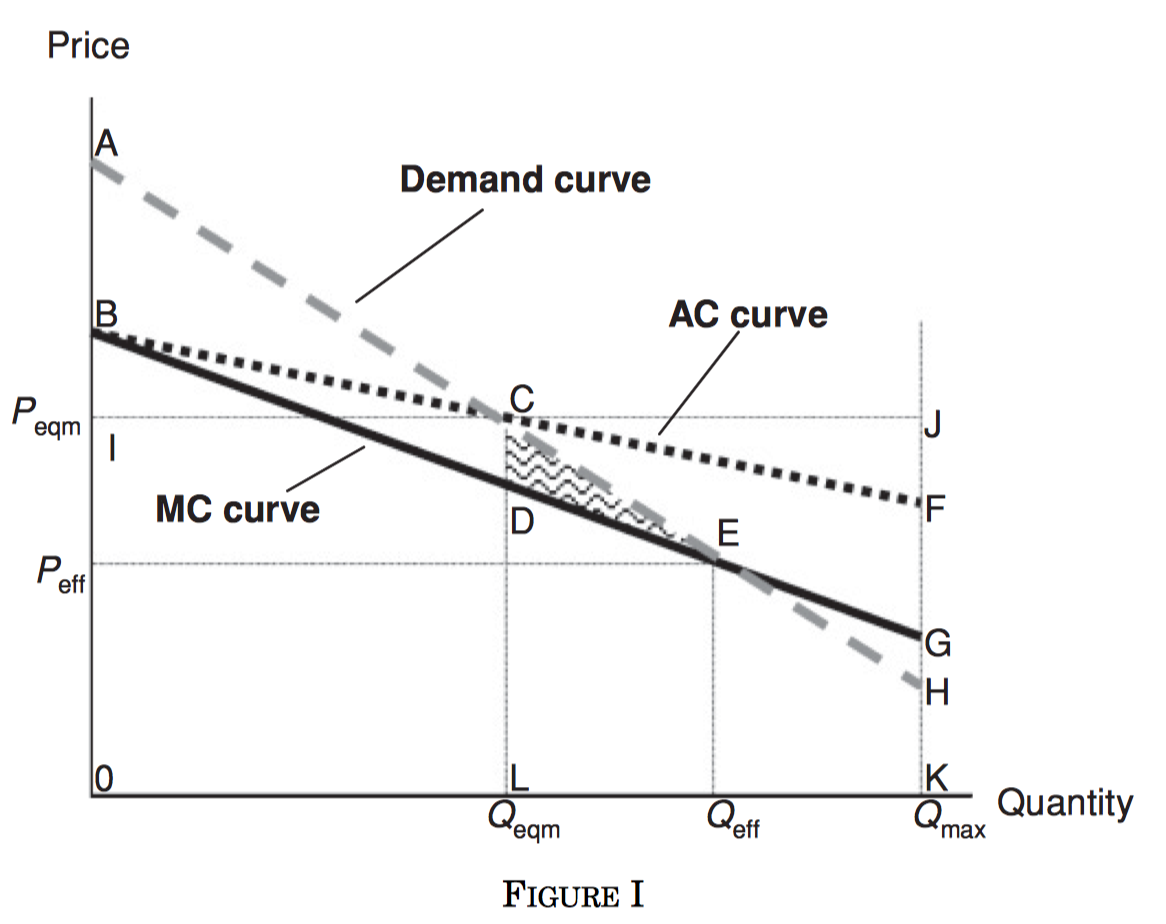
\includegraphics[scale=0.4]{EFC_10qje_1.png}
	\end{figure}

	\begin{figure}[h]
	\centering
	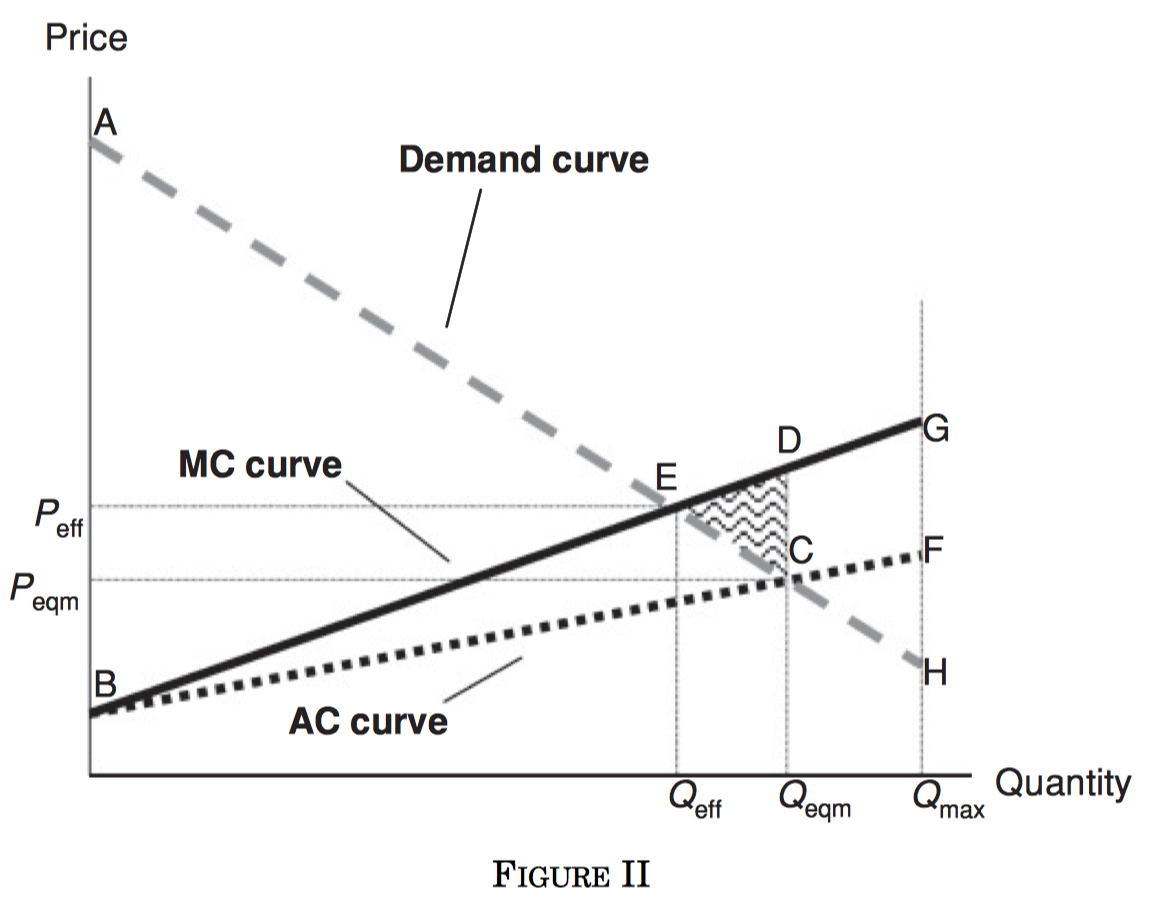
\includegraphics[scale=0.4]{EFC_10qje_2.png}
	\end{figure}

	The adverse selection effect is totally represented by the downward sloping MC/AC curve. If it is advantageous selection, the MC/AC curve will be upward. 
\end{itemize}


\vspace{1em}
\noindent
\textbf{Empirical Results:}
\begin{itemize}
	\item 
\end{itemize}

\vspace{1em}
\noindent
\textbf{Pros:}
\begin{itemize}
	\item This approach has very low demanding on data. Researchers only need \textit{exogenous price change} to get the MC and demand curve. Such change is easy to obtain in insurance industry.
\end{itemize}

\vspace{1em}
\noindent
\textbf{Cons:}
\begin{itemize}
	\item 
\end{itemize}


% subsection einav_finkelstein_cullen_10 (end)



% section asymmetric_information (end)



\chapter{Production Function Estimation} % (fold)
\label{cha:production_function_estimation}

There are several difficulties in estimating production functions which will cause endogeneity problem. To name some:
\begin{itemize}
	\item Simultaneity. For a production function like $y_{it}=\beta_0+\beta_1 k_{it}+\beta_2 l_{it} + \omega_{it}+\varepsilon_{it}$, we suppose that $\omega_{it}$ is obseved by firm but not by econometricians, and $\varepsilon_{it}$ is observed neither by firm nor econometricians. This could induce endogeneity when directly using OLS. 
	Suppose $\omega_{it}$ has \textit{positive serial correlation}, when $\omega_{it}$ is high, firm will choose higher input because it is very possible that $\omega$ in next period will be high as well. This induces a positive bias for $\beta_k$.
	\item Exit selection bias. When constructing a balanced panel, then we only observe those firms with high $\omega_{it}$.
	\textcolor{blue}{Why we have to construct a balanced panel?}
\end{itemize}

There are several approaches in solving this problem.

\begin{itemize}
	\item Classical Approach.
	\begin{itemize}
		\item Use input price as IV. The problem is input price is generally the same across firms. When we do observe different input prices, which generally indicates market power in input markets. Thus those facing higher $\omega_i$ will tend to produce more, inducing their input price to increase, which has a negative bias on $\beta_k$.
		\begin{itemize}
			\item (My comment) When using input price as IV, we actually assume they are independent of individual firm productivities.
			This may not be the case.
			If productivity has some correlation across the firms,
			then it is possible that when productivity is high,
			the input price in the market will also be high.
		\end{itemize}
		\item Use fixed effect. We need to assume that a firm faces same $\omega_{it}$ across time, which is not very practical.
	\end{itemize}
	\item Control Function for  $\omega_{it}$. This approach first raised by \cite{Olley:1996ef} and developed by \cite{Levinsohn:2003ej} and \cite*{Ackerberg:2015ha}. We name them OP, LP, ACF here after. The key idea is to use a function of what we know (for example, $k_t$ and $i_{t-1}$ in OP) to proxy $\omega$, the existence of such function is guaranteed by the solutioin property of the firm optimization problem. And the specific form of this function is estimated non-parametrically.
	\begin{itemize}
		\item OP uses a two step estimation process. First step, use $k_t$ and $i_{t}$ non-parametrically estimate $\omega_t$, plug this into original production function then use OLS. Notice the unobserved $\omega_t$ has been controlled by $k_t$ and $i_{t}$, then OLS will give consistent estimator for $l_t$ but not $k_t$. In second step, we first write $\omega_{it} = E[\omega_{it}|\omega_{it-1}]+\xi_{it}$, notice that $\xi_{it}$ is independent of any information set at t-1. Thus we get the moment condition $E[\xi_{it}k_{it}]=0$, then we can use method of simulating moments to estimate $\beta_k$.
		\begin{itemize}
			\item The key assumption in first step is, current period investment $i_t$ can be represented by a function of $f(k_t,\omega_t)$. 
			If $f$ is invertible in $\omega_t$ (for example, $f$ being monotone in $\omega$), then we can write $\omega$ as a function of $(i_t, k_t)$.
		\end{itemize}

		\item LP is very similar to OP, just that use intermediate input $m_{it}$ instead of investment $i_{it}$ in proxy $\omega_{it}$. Because OP approach requires the policy function of $i_{it}$ be monotonicity in $\omega_{it}$, which is obviously unsatisfied when $i_{it}=0$. But data shows that in many observations $i=0$. Using intermediate input can solve this.

		\item ACF criticizing is that $\beta_l$ cannot be identified in the first step. In LP we assume that $m_{it}=f_t(k_{it},\omega_{it})$. But we can reasonably argue by the same reason that $l_{it}=h_t(k_{it},\omega_{it})$. Then since $f(\cdot)$ is invertible, then we can write $l_t$ as some deterministic function of $k_{it}$ and $m_{it}$. This implies we cannot identify $\beta_l$ in the first step. The solution of ACF is to identify both $\beta_k$ and $\beta_l$ simultaneously at step 2, which is feasible since we now have two moment conditions.
	\end{itemize}
	\item \cite*{Gandhi:2017un} Approach (GNR). GNR criticizes control function approach is nonparametrically not identified in the presence of flexible inputs. They raise a new approach using FOC conditions.
\end{itemize}


% section production_function_estimation (end)









\chapter{Multisided Platforms} % (fold)
\label{cha:multisided_platforms}

\textbf{\bibentry{Evans_Schmalensee:2012wp} }
\begin{itemize}
	\item Price structure matters. Reduce charge by one side and increase charge by another side will affect the transaction.
	\item Transaction cost is necessarily high for multisided platform.
	\item Two kind of externalities. Usage externality and membership externality.
	\item Pricing is compelicated. Per-transaction fee, or membership-fee. \textcolor{blue}{This looks similar to conventional IO model.}
	\begin{itemize}
		\item In per-transaction fee case. Price is directly proportional to the elasticity, while in conventional models price is inversely related to elasticity.
		\[\frac{p_1+p_2-c_1-c_2}{c_1+c_2}=\frac{1}{e_1+e_2}\]
		\[\frac{p_1}{e_1}=\frac{p_2}{e_2}\]
		Notice the second equation is unconventional.
		\item In membership-fee case.
		\item Both models can lead to a highly skewed price structure.
	\end{itemize}
	\item Competition Structure.
	\begin{itemize}
		\item Product differentiation
		\item Multi-home.
		\item Asymetric Competition. A n-sided platform may face competition from 1) one-sided firms; 2) a multisided platform competing in some but not all sides; 3) a multisided platform that has additional sides
	\end{itemize}
\end{itemize}


\myline

\textbf{Random Ideas}
\begin{itemize}
	\item Multisided platform as a commitment device changes the game structure. Like in the Truck-GasStation case raised in the book, the fleet-card company provides commitment power to the card companny, no renegotiation problem.
\end{itemize}

% section multisided_platforms (end)


\chapter{Product Reviews} % (fold)
\label{cha:product_reviews}

\textbf{\bibentry{Berger:2010es}}

\vspace{1em}
\noindent
\textbf{Question and Explanations:}
\begin{itemize}
	\item Why negative reviews may have positive effect on selling?

	\item Negative review may increase awareness of the product.
	\begin{itemize}
		\item Theory prediction: negative reviews should have more negative effect for high awareness products than for low awareness products.
	\end{itemize}

	\item Cannot explain: why some established bad movies like \textit{Fu Chun Shan Ju Tu} still sell a lot.
	\begin{itemize}
		\item May because the different taste between reviewers and mass watchers.
		\item As a social topic, just to be fashion.
	\end{itemize}
\end{itemize}


% section product_reviews (end)



\section{Gentzkov-Shapiro-Taddy, 17 WP} % (fold)
\label{sec:gentzkov_shapiro_taddy_17_wp}


\textbf{\bibentry{Gentzkow:2017hb}}

\begin{itemize}
	\item Methods for analyzing high-dimensional choices decisions
	\begin{itemize}
		\item also see \bibentry{Gentzkow_el.al:17WP}
	\end{itemize}
	\item Index for measuring polarization
\end{itemize}


This is a methodology paper introducing how to analyze high-dimensional choices decisions. They show that traditional logit model has severe finite sample bias.
They also raise a index for measuring polarization.

\textcolor{red}{[TO BE ADDED]}

% section gentzkov_shapiro_taddy_17_wp (end)


\chapter{Others} % (fold)
\label{cha:others}

\textbf{\bibentry{Einav:2010cd}}

This survey paper provides a map for current empirical IO research, its range, and its relationship to theory.
In addition, the ending part has a critique on the `reduced' view on IO (e.g. Angrist), worth reading.


\subsection{Rey and Stiglitz, 1995, RAND} % (fold)
\label{subsec:rey_and_stiglitz_1995_rand}

\textbf{\bibentry{Rey:1995ft}}

For detailed proof of this paper, see Evernote.\\

\textbf{Main result:}
vertical restrains can be used to reduce interband competition. Because exclusive territories alter the perceived demand curve, making each producer believe he faces a less elastic demand curve, inducing an increase in eqm price and producer's profits even in the abscence of franchise fee. This result is different from traditional Chicago school results, which insist that exclusive terittories will increase efficiency. This difference comes from market structure. Chicago schools investigate in full competition and full monopoly producer cases, while this paper looks at duopoly producer. In full competition and full monopoly case, the competition level has already been \textit{preassumed}, while exclusive territories can reduce the competition level among producers in other cases.\\

The key for the result is the the following compound demand elastic:
\[\tilde\varepsilon(p^e):=m_1(p,p)\varepsilon_1(q,q)+m_2(p,p)\varepsilon_2(q,q) \]
where $q=q_1^r(p,p)$ (the response retail price),
$m_1(p,p)=\partial \log q_1^r(p_1,p_2)/\partial \log p_1$ (the own elasticity of retail price to producer price),
and  $m_2(p,p)=\partial \log q_1^r(p_1,p_2)/\partial \log p_2$ (the cross elasticity of retail price to producer price),
and $\varepsilon_1(q_1,q_2)=-\partial \log D^1(q_1,q_2)/q_1$ (the own elasticity of demand to retail price, positive),
and $\varepsilon_2(q_1,q_2)=-\partial \log D^1(q_1,q_2)/q_2$ (the cross elasticity of demand to retail price, negative).

In the above equation, it is very reasonable to think $0<m_1<1$ and $0<m_2$. $m_1>0$ because the own elasticity of retail price to producer price is positive. $m_1<1$ means that retailer will absorb some increase in producers' price, which will be the case if demand elasticity becomes higher in high retail price. And $0<m_2$ derives from the two products to be substitutes. Under these two conditions, combined with $\varepsilon_1>0$ and $\varepsilon_2<0$, then $\tilde\varepsilon(p^e)<\varepsilon_1$. Thus, under exclusive territories, the producers' perceived demand curve is less elastic. So the equilibrium price (both retail and producer) is higher even when no franchise fee applies.

\noindent
\textbf{Setting:}

\begin{itemize}
	\item two manufacturers produce imperfect substitutes at same marginal cost \textit{c}
	\item retailers are perfect competition / or exclusive territory
	\item the final good demand depends on retail prices and is given by $D^i(q_1,q_2)$
	\item costs and demand functions are common knowledge, retailers observe all contracts signed by each producer
	\item producers only observer the quantity bought by retailers; they do not observe the quantities sold by retailers (i.e. fullline forcing is infeasible)
	\item producers serve many markets at no addtional cost
	\item consumers have no search cost
\end{itemize}

Under these settings and information conditions, we can see it as a two stave game. In the first stage, producers simultaneously set wholesale price $p_1$ and $p_2$. In the second stage, the retailer observe all wholesale price and decide the retail price simutaneously.

\subsubsection{Benchmark Case} % (fold)
\label{sub:benchmark}

We use the following assumptions throughout the paper unless specified otherwise:

\begin{enumerate}
	\item Let $\pi(p_i,q_1,q_2) := (q_i-p_i)D^i(q_1,q_2)$ denote the retail profit for product i; assume it to be twice differentiable wrt each argument, and is sigle peaked wrt $q_i$. The reaction function $q_i^a(p_i,q_j)$ is thus continously differentiable and characterized by FOC.
	\item Products are substitutes: $\partial D^i/\partial q_i \leq 0$ and $\partial D^i/\partial q_j \geq 0$
	\item Demand functions are symmetric: $\forall p_1,p_2 \in \R_+, D^1(p_1,p_2) = D^2(p_2,p_1)$
\end{enumerate}

Think of the benckmark case that no vertical restriction so the retailers are perfect competitive, and the producer monopolizes. In this case, the game is just a one step optimal pricing problem. The producer chooses an optimal retail price.\\

\begin{mdframed}[style=comment]

\noindent
\textbf{Useful trick:}

Throughout this paper, we can write the symmetric eqm conditions in the following form:
\[(p^c - c)/p^c=1/\varepsilon(p^c,p^c)\]
where $p^c$ is the symmetric eqm price, and $\varepsilon$ is some kind of elasticity.

In a symmetric eqm, the FOC of each producer gives 
\((p^c - c)/p^c=1/\varepsilon_1(p^c,p^c)\)
where $\varepsilon_1 = -\partial \log D^1(q_1,q_2)/\partial \log q_1$, i.e. the self elasticity of demand.

In the simplest benchmark case, the two factories are integrated, leading us to:
\((p^c - c)/p^c=1/E(q^m)\),
$E(q):=\varepsilon_1(q,q)+\varepsilon_2(q,q)$, where $\varepsilon_2 = -\partial \log D^1(q_1,q_2)/\partial \log q_2$ (the cross demand elasticity).

In the exclusive territory case, the symmetric eqm satisfies \((p^e - c)/p^e=1/\tilde\varepsilon(p^e)\), where 
\[\tilde\varepsilon(p^e):=m_1(p,p)\varepsilon_1(q,q)+m_2(p,p)\varepsilon_2(q,q) \]
where $q=q_1^r(p,p)$ (the response retail price),
$m_1(p,p)=\partial \log q_1^r(p_1,p_2)/\partial \log p_1$ (the own elasticity of retail price to producer price),
and  $m_2(p,p)=\partial \log q_1^r(p_1,p_2)/\partial \log p_2$ (the cross elasticity of retail price to producer price).

\end{mdframed}



% section others (end)

\part{Trade and Spatial Economics} % (fold)
\label{prt:trade_ _and_ _spatial_ _economics_}

\chapter{Trade Basic Model} % (fold)
\label{cha:trade_basic_model}


\section{CES Functions} % (fold)
\label{sec:ces_functions}

\subsection{CES Utility (discrete)} % (fold)
\label{sub:ces_utility_discrete}

Reference: Rutherford (2002), Lecture Notes on Constant Elasticity Functions

The CES utility function is defined as:
\[U ( x , y ) = \left( \alpha x ^ { \rho } + ( 1 - \alpha ) y ^ { \rho } \right) ^ { 1 / \rho }\]
We can calculate the demand:
\[\begin{array} { c } { x \left( p _ { x } , p _ { y } , M \right) = \left( \frac { \alpha } { p _ { x } } \right) ^ { \sigma } \frac { M } { \alpha ^ { \sigma } p _ { x } ^ { 1 - \sigma } + ( 1 - \alpha ) ^ { \sigma } p _ { y } ^ { 1 - \sigma } } } \\ { y \left( p _ { x } , p _ { y } , M \right) = \left( \frac { 1 - \alpha } { p _ { y } } \right) ^ { \sigma } \frac { M } { \alpha ^ { \sigma } p _ { x } ^ { 1 - \sigma } + ( 1 - \alpha ) ^ { \sigma } p _ { y } ^ { 1 - \sigma } } } \end{array}\]
and also the indirect utility:
\[V \left( p _ { x } , p _ { y } , M \right) = M \left( \alpha ^ { \sigma } p _ { x } ^ { 1 - \sigma } + ( 1 - \alpha ) ^ { \sigma } p _ { y } ^ { 1 - \sigma } \right) ^ { \frac { 1 } { \sigma - 1 } }\]
$V$ is homogeneous of degree 1 in M. This permits us to form an exact \textbf{price index} corresponding to the cost of a unit of utility:
\begin{align*}
	1 \equiv V(p_x,p_y,e(p_x,p_y,V=1)) = e(p_x,p_y,V=1)\left( \alpha ^ { \sigma } p _ { x } ^ { 1 - \sigma } + ( 1 - \alpha ) ^ { \sigma } p _ { y } ^ { 1 - \sigma } \right) ^ { \frac { 1 } { \sigma - 1 } } \\
	\Rightarrow e(p_x,p_y) \equiv e(p_x,p_y,V=1) = 
	\left( \alpha ^ { \sigma } p _ { x } ^ { 1 - \sigma } + ( 1 - \alpha ) ^ { \sigma } p _ { y } ^ { 1 - \sigma } \right) ^ { \frac { 1 } {1- \sigma } }
\end{align*}
The indirect utility can be reframed as:
\[V(p_x,p_y,M) = \frac{M}{e(p_x,p_y)}\]
Importantly, wlog, we can think of each consumer demand only one good, and $e(p_x,p_y)$ is the price index for that good.


\mysubtitle{Elasticity:}

CES get its name because the cross elasticity is a constant independent of consumption bundle. To see this we first use a more general form:
\[U(\vec x) = \left[ \sum_{i=1}^n x_i^\rho \right]^{\frac{1}{\rho}}\]
By brutal force calculation we get:
\[\frac{\partial x_i/ x_i}{\partial p_j / p_j} = \frac{1}{1-\rho}\]
% subsection ces_utility (end)

\subsection{CES Utility (continuous)} % (fold)
\label{sub:ces_utility_}

CES can be generated to continuous version:
\[\begin{aligned} \max U ( \mathbf { c } ) & = \left( \int _ { 0 } ^ { 1 } b ( i ) c ( i ) ^ { \rho } d i \right) ^ { 1 / \rho } \\ \text { s.t. } & \int _ { 0 } ^ { 1 } p ( i ) c ( i ) d i = I \end{aligned}\]
Write the Lagranian and we have FOC:
\begin{align*}
	b(\iota)\rho c(\iota)^{\rho-1} \frac{1}{\rho} \left( \int _ { 0 } ^ { 1 } b ( i ) c ( i ) ^ { \rho } d i \right) ^ { (1-\rho) / \rho }
	= \lambda p(\iota) \\
	b(\iota)c(\iota)^{\rho-1} \left( \int _ { 0 } ^ { 1 } b ( i ) c ( i ) ^ { \rho } d i \right) ^ { (1 - \rho )/ \rho } 
	= \lambda p(\iota),\ \forall \iota \in [0,1] \tag{2}
\end{align*}
Multiply both sides by $c(\iota)$ and take integration:
\begin{align*}
	\left( \int _ { 0 } ^ { 1 } b ( i ) c ( i ) ^ { \rho } d i \right) ^ { ( 1 - \rho ) / \rho }
	\left( \int _ { 0 } ^ { 1 } b ( \iota ) c ( \iota ) ^ { \rho } d \iota \right) 
	= \lambda \int _ { 0 } ^ { 1 } p ( \iota ) c ( \iota ) d \iota = \lambda I\\
	\left( \int _ { 0 } ^ { 1 } b ( i ) c ( i ) ^ { \rho } d i \right) ^ { 1 / \rho } = \lambda I
\end{align*}
Define the LHS as $C$, the composite consumption, $P\equiv\lambda^{-1}$ and we will get:
\[CP = I\]
we call $P$ the \textbf{price index}, which has a natural interpretation to be the price of a unit util. 
It should be noted that here $C$ is already the \textit{optimal} consumption bundle. 

We still need to solve $P$. Return to (2) and solve $c(\iota)$:
\[
c(\iota) = 
\left[b(\iota)^{-1} \left( \int _ { 0 } ^ { 1 } b ( i ) c ( i ) ^ { \rho } d i \right) ^ { ( \rho -1) / \rho } \lambda p(\iota)
\right]^{\frac{1}{\rho-1}}
\]
\begin{align*}
	b(\iota)c(\iota)^{\rho} &= 
b(\iota)\left[b(\iota)^{-1} \left( \int _ { 0 } ^ { 1 } b ( i ) c ( i ) ^ { \rho } d i \right) ^ { ( \rho -1) / \rho } \lambda p(\iota)
\right]^{\frac{\rho}{\rho-1}}\\
&= b(\iota)^{\frac{-1}{\rho-1}}\left(\lambda p(\iota)\right)^{\frac{\rho}{\rho-1}} \int _ { 0 } ^ { 1 } b ( i ) c ( i ) ^ { \rho } d i
\end{align*}
Taking integral in both sides:
\begin{align*}
	1 = 
	\lambda^{\frac{\rho}{\rho-1}}
	\int_0^1 b(\iota)^{\frac{-1}{\rho-1}} p(\iota)^{\frac{\rho}{\rho-1}} d \iota\\
	P \equiv \lambda^{-1} = \left[\int_0^1 b(\iota)^{\frac{-1}{\rho-1}} p(\iota)^{\frac{\rho}{\rho-1}} d \iota\right]^{\frac{\rho-1}{\rho}}
\end{align*}

\mytitle{Properties}

\mysubtitle{Cross Elasticity:}

By equation (2), take the log form and take partial derivative, we get:
\[
\sigma  \equiv \frac{\partial c(x)/ c(x)}{\partial p(y)/p(y)} = \frac{1}{\rho-1}\]

\mysubtitle{Own Elasticity:}

Still from (2), we substitute $\lambda$ by $P^{-1}$. Then (2) can be written as:
\begin{align*}
	b(\iota)c(\iota)^{\rho-1}C^{1-\rho} = P^{-1}p(\iota)\\
\end{align*}
The trick is that a single product $c$ is so small that it will affect neither $C$ nor $P$. And thus the own elasticity is still $\frac{1}{\rho-1}$.

\mysubtitle{Limiting Cases:}

When $\rho \rightarrow 0$, Cobb-Douglas. When $\rho \rightarrow 1$, perfect substitution. When $\rho \rightarrow \infty$, Leontief.
\blue{This is from Kim Ruhl's notes, I did not check.}


\mysubtitle{Two Stage Budgeting:}

Suppose there is some outside good $c_0$ in the economy:
\[\begin{array} { c } { \max U \left( c _ { 0 } , \left( \int _ { 0 } ^ { 1 } b ( i ) c ( i ) ^ { \rho } d i \right) ^ { 1 / \rho } \right) } \\ { \text { s.t. } p _ { 0 } c _ { 0 } + \int _ { 0 } ^ { 1 } p ( i ) c ( i ) d i = I } \end{array}\]
One thing important is that the differentiated goods can be aggregated into one commodity $C$. Then the above problem can be summarized as a two stage problem.
\[\begin{array} { c } { \max U \left( c _ { 0 } , C \right) } \\ { \text { s.t. } p _ { 0 } c _ { 0 } + P C = I } \end{array}\]
We first solve $C$ and $PC$. Then everything comes similar.
% subsection ces_utility_ (end)

% section ces_functions (end)



\section{Ricardian Model} % (fold)
\label{sec:ricardian_model}

This representation is based on DFS 1977.

\mytitle{Settings:}
\begin{itemize}
	\item Two countries: Home and Foreign
	\item One factor of production
	\begin{itemize}
		\item This is important in Ricardian model, because the order of $z$ below relies on unique factor of production. Otherwise we won't have a meaningful order.
		\item Denote $L, L^*$ as the labor endowments in two countries; and $w, w^*$ be the wages respectively. All terms are real.
	\end{itemize}
	\item A continuum of goods indexed by $z \in [0,1]$
	\begin{itemize}
		\item A continuum of $z$ is easier to deal with than discrete $z$.
	\end{itemize}
	\item Technology: $a(z)$ and $a^*(z)$ are the labor requirements for produing unit good.
	\begin{itemize}
		\item Order goods s.t. $A(z)\equiv \frac{a^*(z)}{a(z)}$ is decreasing. So Home has comparative advantage in low $z$.
	\end{itemize}
\end{itemize}

\mytitle{Equilibrium:}
\begin{itemize}
	\item Suppose there is no trade cost. Let $p(z)$ denote the (home) price of good $z$ under free trade.
	\item Since the competition is perfect, and there is no trade cost, the product will be produced in the country with lower labor cost:
	\[\begin{aligned} p(z)-w a(z) & \leq 0, \text {w . equality if } z \text { is produced at Home }(1) \\ p(z)-w^{*} a^{*}(z) & \leq 0, \text { w. equality if } z \text { is produced Abroad }(2) \end{aligned}\]
	\item A direct proposition is: there exists $\tilde z$ s.t. Home produces all goods $z<\tilde z$ and vice versa for Foreign.
	Another result is: $A(\tilde z) = \frac{w}{w^*}\equiv \omega$. Note that $\omega$ is endogenous and can be calculated in equilibrium.
	\item To calculate $\omega$, we further assume consumers have \textbf{identical Cobb Douglas} preference around the world. Then we denote $b(z)$ the share of expenditure on good $z$: (which actually should be understand as density of share):
	\[
	b(z)=\frac{p(z) c(z)}{w L}=\frac{p(z) c^{*}(z)}{w^{*} L^{*}}
 	\]
 	by def, shares should satisfy:
 	\[\int_{0}^{1} b(z) d z=1\]
 	Let $\theta(\widetilde{z}) \equiv \int_{0}^{\widetilde{z}} b(z) d z$ denote the fraction of income spent on goods produced at Home. Trade balance requires Home Exports = Home Imports:
 	\[\theta(\widetilde{z}) w^{*} L^{*}=[1-\theta(\widetilde{z})] w L\]
 	then we have relative wage to be:
 	\[\omega=\frac{\theta(\widetilde{z})}{1-\theta(\widetilde{z})}\left(\frac{L^{*}}{L}\right) \equiv B(\widetilde{z})\]
 	Notice this is an GE results. An technical advancement will increase $\tilde z$, which must be compensated by an increase in $\omega$ in equilibrium.
\end{itemize}

\mytitle{Comparative Statics:}
\begin{itemize}
	\item Below figure plots the equilibrium.$A(z)$ is downward by construction, $B(z)$ is upward by above equation.

	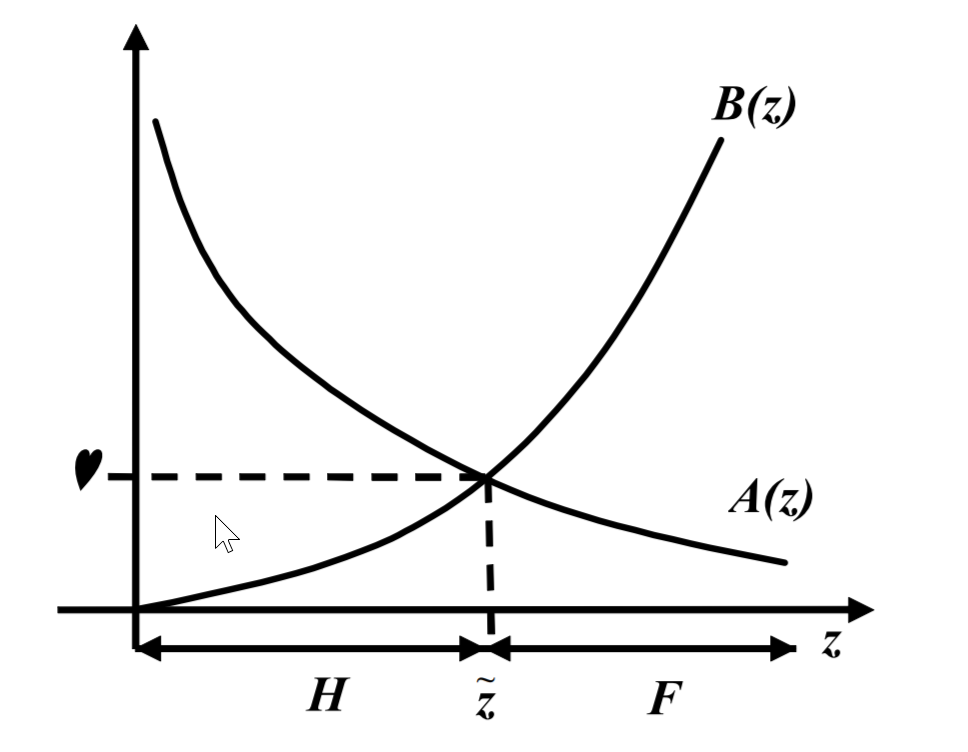
\includegraphics[width=0.5\linewidth]{images/ricardian.png}
	\item Suppose $L^*/L$ increases, how it will change equilibrium price and welfare?
	\begin{itemize}
		\item For notation ease, set $w=1$ wlog since it only serves as numerair.
		\item First notice that $\omega$ increases and $\tilde z$ decreases in equilibrium.
		\item For goods produced at Home, no change in $p(z)$ since it only depends on Home technology.
		\item For goods whose production remains at Abroad:
		\[\omega \nearrow \Rightarrow w^{*} \searrow \Rightarrow p(z)=w^{*} a^{*}(z) \searrow\]
		\item For goods moved to be produced Abroad, then by profit optimization:
		\[w^{*} a^{*}(z) \leq a(z) \Rightarrow p(z) \searrow\]
		\item Thus Home gains.
	\end{itemize}
	\item KZ: The Abroad welfare decreases because of population increase. Why does this happen? Because Abroad now produces goods that they have less comparative advantages. They produce these goods because they have low wage, due to the competition effect of large population.

\end{itemize}



% section ricardian_model (end)


\section{Eaton and Kortum, 02 EMCA} % (fold)
\label{sec:eaton_and_kortum_02_emca}

\mytitle{Setting:}
\begin{itemize}
	\item Efficiency: country $i$'s efficiency in product $j$ is $z_i(j)$
	\item Input price in country $i$ is $c_i$, which can be further decomposed into labor cost and intermediate inputs cost
	\item Geographic barriers between country $i$ and country $n$ is $d_{ni}$. \red{Is $d_{ni}$ symmetric?}
	\item Production cost is:
	\[p _ { n i } ( j ) = \left( \frac { c _ { i } } { z _ { i } ( j ) } \right) d _ { n i }\]
	which is also the purchase cost by perfect competition assumption. However, the buyer will buy from the cheapest seller, and we assume the search is costless:
	\[p _ { n } ( j ) = \min \left\{ p _ { n i } ( j ) ; i = 1 , \ldots , N \right\}\]
	\item Utility: buyers have the love of variety, and we assume a CES utility form:
	\[U = \left[ \int _ { 0 } ^ { 1 } Q ( j ) ^ { ( \sigma - 1 ) / \sigma } d j \right] ^ { \sigma / ( \sigma - 1 ) }\]
	where the elasticity of substitution is $\sigma>0$.
\end{itemize}

\mysubtitle{Technology:}
\begin{itemize}
	\item The technology $z_i(j)$ is the realization of r.v. $Z_i$, drawn independently for each product $j$. $Z_i$ follows a Type II extreme value distribution:
	\[F _ { i } ( z ) = e ^ { - T _ { i } z ^ { - \theta } }\]
	$T_i$ governs the location of distribution, and $\theta$ common for all countries governs the variation \textit{within} the distribution. A bigger $\theta$ represents less variability.
	\blue{This distribution is the key to the closed form solution.}
\end{itemize}

\mysubtitle{Prices:}
\begin{itemize}
	\item The induced price distribution is:
	\begin{align*}
		G _ { n i } ( p )
		& = \Pr \left( P _ { n i } ( j ) \leq p \right) \\
		& =  \Pr(\frac{c_i}{z_i(j)}d_{ni} \leq p) \\
		& = 1-F_i(\frac{c_i d_{ni}}{p}) \\
		& = 1 - e^{-T_i(c_i d_{ni})^{-\theta}p^{\theta}}
	\end{align*}
	The purchasing price distribution is thus: \red{how to derive?}
	\begin{align*}
		G _ { n } ( p ) & = 1 - \prod _ { i = 1 } ^ { N } \left[ 1 - G _ { n i } ( p ) \right] \\
		& = 1 - e ^ { - \Phi _ { n } p ^ { \theta } }
	\end{align*}
	where $\Phi_n$ is:
	\[\Phi _ { n } = \sum _ { i = 1 } ^ { N } T _ { i } \left( c _ { i } d _ { n i } \right) ^ { - \theta }\]

	\item The probability that country $i$ provides a good at the lowest price in country $n$ is:
	\begin{align*}
	\pi _ { n i } &= \operatorname { Pr } \left[ P _ { n i } ( j ) \leq \min \left\{ P _ { n s } ( j ) ; s \neq i \right\} \right] \\
	& = \int _ { 0 } ^ { \infty } \prod _ { s \neq i } ^ { \infty }  \left[ 1 - G _ { n s } ( p ) \right] d G _ { n i } ( p ) \\
	&= \frac { T _ { i } \left( c _ { i } d _ { n i } \right) ^ { - \theta } } { \Phi _ { n } }
	\end{align*}
	\red{the last step?}

	\item The price of a good that country $n$ \textit{actually buys} from country $i$ also has the distribution $G_n(p)$. This means that the price distribution \textit{conditional} on export country is the same as overall price distribution faced by importer country $n$. This result can be derived by showing that:
	\[G _ { n } ( p ) = \frac { 1 } { \pi _ { n i } } \int _ { 0 } ^ { p } \prod _ { s \neq i } \left[ 1 - G _ { n s } ( q ) \right] d G _ { n i } ( q )\]

	\item The price index for CES function is then \red{(why?)}
	\[p _ { n } = \gamma \Phi _ { n } ^ { - 1 / \theta } \tag{9}\]
	where 
	\[\gamma = \left[ \Gamma \left( \frac { \theta + 1 - \sigma } { \theta } \right) \right] ^ { 1 / ( 1 - \sigma ) }\]
	$\Gamma$ is the gamma function.
	
\end{itemize}


\mysubtitle{Trade Flows and Gravity}
\begin{itemize}
	\item Since the price distribution conditional on source is the same as overall price distribution, a corollary is that the average expenditure per good is identical across sources. Thus, the fraction of goods that country $n$ buys from country $i$, $\pi_{ni}$ is the fraction of expenditures:
	\[\frac { X _ { n i } } { X _ { n } } = \pi_{ni} = \frac { T _ { i } \left( c _ { i } d _ { n i } \right) ^ { - \theta } } { \Phi _ { n } } = \frac { T _ { i } \left( c _ { i } d _ { n i } \right) ^ { - \theta } } { \sum _ { k = 1 } ^ { N } T _ { k } \left( c _ { k } d _ { n k } \right) ^ { - \theta } } \tag{10}\]
	The exporter's total sales $Q_i$ are:
	\[Q _ { i } = \sum _ { m = 1 } ^ { N } X _ { m i } = T _ { i } c _ { i } ^ { - \theta } \sum _ { m = 1 } ^ { N } \frac { d _ { m i } ^ { - \theta } X _ { m } } { \Phi _ { m } }\]
	Then we can cancel out $T_i c_i^{-\theta}$:
	\[T_i c_i^{-\theta} = 
	\frac{X_{ni}\Phi_n d_{ni}^\theta}{X_n} = 
	\frac{X_{ni}}{X_n} \left(\frac{p_n}{\gamma d_{ni}}\right)^{-\theta}\]
	the second equation is from derived CES price index equation. Substitute $T_i c_i^{-\theta}$ into $Q_i$ and we get:
	\[X _ { n i } = \frac { \left( \frac { d _ { n i } } { p _ { n } } \right) ^ { - \theta } X _ { n } } { \sum _ { m = 1 } ^ { N } \left( \frac { d _ { m i } } { p _ { m } } \right) ^ { - \theta } X _ { m } } Q _ { i } \tag{11}\]
	\blue{Why we are interested in this equation?} Because it resembles the standard gravity equation.

\end{itemize}


\mytitle{Trade, Geography and Price: The Connection:}
\begin{itemize}
	\item Notice that if we divide (10) by $X_{ii}/X_i$, we get:
	\[\frac { X _ { n i } / X _ { n } } { X _ { i i } / X _ { i } } = \frac { \Phi _ { i } } { \Phi _ { n } } d _ { n i } ^ { - \theta } = \left( \frac { p _ { i } d _ { n i } } { p _ { n } } \right) ^ { - \theta }\]
	the LHS is called \textit{normalized import share}. \red{why we want to normalize it?}
\end{itemize}


\mytitle{Input Costs:}

\mysubtitle{Production:}
\begin{itemize}
	\item The cost of an input bundle in country $i$ is:
	\[c _ { i } = w _ { i } ^ { \beta } p _ { i } ^ { 1 - \beta }\]
\end{itemize}

% section eaton_and_kortum_02_emca (end)

% chapter trade_basic_model (end)

% part trade_ _and_ _spatial_ _economics_ (end)


% chapter io (end)

\part{Micro Theory} % (fold)
\label{prt:micro_ _theory_}

% part micro_ _theory_ (end)

\chapter{Game Theory} % (fold)
\label{cha:game_theory}

\section{Important Tools} % (fold)
\label{sec:important_tools}

\begin{thm}[Revelation Principle, Myerson, 1981]
Suppose that $\psi$ was a Bayes Nash equilibrium of the indirect mechanism $\Gamma$. 
Then there exists a direct mechanism that is payoff-equivalent and where truthful revelation is an equilibrium.
\end{thm}

\begin{myproof}
[to be added]
\end{myproof}

\begin{singlespacing}
\noindent
\textit{Comment:}
\end{singlespacing}
\begin{itemize}
	\setlength{\itemsep}{0pt}
	\item Revelation Principle is defined over some specific solution concept. Here it is Bayes Nash Eqm.
	\item Revelation principle is not always satisfied. The stronger solution concept we use, the more likely it is not satisfied.
\end{itemize}


\subsection{Solution Concept} % (fold)
\label{sec:solution_concept}

A very good reference for different solution concept is \cite{vanDamme:1987}.
\begin{itemize}
	\item Nash eqm
	\item Subgame Perfect eqm
	\item Perfect eqm
	\item $\varepsilon$-Perfect eqm
	\item Proper eqm
	\item Trembling-Hand eqm
	\item Bayesian Nash eqm
	\item (Weak) Perfect Bayesian eqm
	\item Sequential eqm
	\item Forward looking eqm
	\item Self-Confirming eqm

\end{itemize}


\begin{defn}[Self-confirming Equilibrium, \cite{Fudenberg_Levine:93EMCAa}]
Profile $\sigma$ is a \textit{self-confirming equilibrium} if for each player i, $s_i \in$ support($\sigma_i$) there exists belief $\mu_i$ such that:
\begin{enumerate}
	\item $s_i$ maximizes $u_i(\dot,\mu_i)$, and
	\item $\mu_i[\{\pi_{-i}|\pi_j(h_j)=
	\hat \pi_j(h_j|\sigma_j)\}]=1$, for all $j \neq i$ and $h_j \in \bar H(s_i,\sigma_-i)$, where $\bar H$ is the set of info sets that are reached with positive probability
\end{enumerate}
\end{defn}

\begin{singlespacing}
\noindent
\textit{Comment:}
\end{singlespacing}
\begin{itemize}
	\setlength{\itemsep}{0pt}
	\item This definition mainly requires that the belief $\mu_i$ is consistent only at information sets that are reached with positive probability when player $i$ plays $s_i$.
	\item This is most obvious when contrast with Nash Eqm, which is almost the same as this definition,
	except for the consistency requirement is for all $h_j \in H_{-i}$. The consistency is required  for all information sets.
	\item Self-confirming is a weaker solution concept than Nash Equilibrium. 
	It uses the idea that players can only learn through what they observe.
	For those outcomes that they cannot observe,
	there is no particular reason for their beliefs to coincide.
	Players can never learn something they lack information on.
\end{itemize}

\begin{exmp}

\end{exmp}

% subsection solution_concept (end)

\section{Decision Theory} % (fold)
\label{sec:decision_theory}


\subsection{Morris, 95 Econ\&Phil} % (fold)
\label{sub:morris_95_econ_phil}

% subsection morris_95_econ&phil (end)

\textbf{\bibentry{Morris:1995ic}}

This assumption reviews the common prior assumption in economics, its common justifications, and its impact on game theory.

\textcolor{blue}{VEEY WORTH READING!! NOTES TO BE ADDED.}


% section decision_theory (end)


\section{Mechanism Design} % (fold)
\label{sec:mechanism_design}

\noindent
Important tools and topics in mechanism design:
\begin{itemize}
	\item Revelation Principle
	\item Single dimension mechanism design
	\begin{itemize}
		\item Bayesian mechanism design
		\item Dominant strategy mechanism design
		\item Revenue equivalence
		\item Payoff equivalence
	\end{itemize}
	\item Multidimensional mechanism design
	\item Interdependent types mechanism design
\end{itemize}


\subsection{Revelation Principle} % (fold)
\label{sub:revelation_principle}

There are many things assumed in the proof of revelation principle. Take p.10 in Borger's book as example.

\begin{itemize}
	% \item Assume that in initial game, one can pretend to be someone else. That is, $\sigma(\theta')$ is in the action space of $\theta$.
	\item No verification.
	\item Utility is transferable.
\end{itemize}

For an example where all three assumptions are violated, see \cite*{BenPorath:2014bc}.


\begin{mdframed}[style=comment]
\noindent
\textbf{Information side of Revelation Principle:}

In setting we prove revelation principle, we assume every thing is common knowledge except for the specific type.
These include the type space, the action space of each type, the utility form of each type, and so on. 
We also assume that in the direct mechanism, the action space is the \textit{whole} type space for \textit{every} agents.
\textcolor{red}{[Don't understand this. Since in the proof we only require that one can report truthfully.]}

\end{mdframed}



% subsection revelation_principle (end)

% section mechanism_design (end)



% section important_tools (end)

\section{Learning Theory} % (fold)
\label{sec:learning_theory}

\subsection{Important tools in learning} % (fold)
\label{sub:important_tools_in_learning}

\begin{defn}[Monotone Likelihood Ratio Property]
For all $l<S$,

\[\frac{p_{q,l}}{p_{q+1,l}} \geq \frac{p_{q,l+1}}{p_{q+1,l+1}} \ for \ all \ q<R\]
with strictly inequality for at least one q.

\end{defn}

This is first raised by \cite{Milgrom:1981dv}, which ensures that the conditional expectation of each individual increases in his signal realization.

\begin{defn}[Martingale]
A \textit{martingale} is a pair $(X_n,\F_N)$, where $\{\F_n\}$ is a filtration and $X_n$ an integrable (i.e. $E|X|<\infty$) stochastic process adapted to this filtration, such that 
\[E[X_{n+1}|\mathcal{F}_n]=X_n,\ a.s. \ \forall n\]
\end{defn}

\noindent
\textit{Comment:}
\begin{itemize}
	\setlength{\itemsep}{0pt}
	\item Notice that Martingale process is much more restricted than Markov process, not only in the realization of expectation value. Markov process requires that 
	\[Pr(X_{t+1}\in A)|X_t=x_0,X_{t-1}=x_{t-1},...,X_{t-k}=x_{t-k}
	=Pr(X_{t+1}\in A)|X_t=x_0\]
	for all $A \in \mathcal{X}$, all $x_0,x_1,...,x_k \in \mathbb{X}$, and all $0\leq k\leq t$. 
	\begin{itemize}
		\item This actually restricts all stochastic properties, including expectations, variations and others.
		\item Also, Martingale process require conditional on $\F_t$, but Markov process only requires $x_t$.
	\end{itemize}
\end{itemize}



\begin{thm}[Martingale Convergence Theorem]

\end{thm}



% subsection important_tools_in_learning (end)

\subsection{Overview of literature} % (fold)
\label{sub:overview_of_literature}

% subsection overview_of_literature (end)

\textcolor{red}{The equilibrium concept used in literature is Bayesian Nash Eqm. Thus we put no restriction on off-eqm path beliefs. Nageeb said something about this, but I don't understand why this is important.}

\cite{Bikhchandani:1992fs} (BHW here after) is one of the original papers for learning in games. The main point is to explain the easily formulated but fragile information cascade when only actions are observed. The idea is, if only actions are observed, then after some threshold, private information will not affect action. And this private will NOT join the information pool, thus all following individual's private information will not contribute to the action. But since very little information is needed to form a cascade, this cascade can also be easily reversed when some shocks happen.


\cite{Smith:2000tz} is a generalization of BHW paper. The generalization lies in these aspects:
\begin{itemize}
	\setlength{\itemsep}{0pt}
	\item Heterogeneity in quality of information (possibly unbounded private information)
	\item Heterogeneity of preference (noise by crazy types)
	\item Information cascade is NOT a generic feature; but 'herding' is.
	\item Necessary and sufficient condition for \textit{complete learning}.
\end{itemize}
This paper also provides a general approach on how to handle learning behaviour.
% section learning_theory (end)

\subsection{Bikhchandani-Hirshleifer-Welch, 92 JPE} % (fold)
\label{subsec:bikhchandani_hirshleifer_welch_92_jpe}

\textbf{\bibentry{Bikhchandani:1992fs}}

BHW is the seminal paper of social learning, which explains imitating in social phenomena without any ad hoc assumptions. By ad hoc assumptions, I means following:
\begin{itemize}
	\setlength{\itemsep}{0pt}
	\item sanctions on deviants
	\item positive payoff externalities
	\item conformity preference
\end{itemize}
This assumptions all have the unsatisfying property that puts the cart before the horse.

\textcolor{red}{TO BE ADDED}


% section bikhchandani_hirshleifer_welch_92_jpe (end)


\subsection{Kremer-Mansour-Perry, 14 JPE} % (fold)
\label{subsec:kremer_mansour_perry_14_jpe}

\textbf{\bibentry{KMP:2014jpe}}

Different from previous learning papers, KMP focuses on the optimal information disclosure of planner.
They find that it is not always optimal for planner to disclose full information, because it will discourage agents' incentive to explore and exploration has positive externalities.

Example: Online review website like TripAdvisor, Yelp; Google Map\\

\noindent
\textit{Illustrative example:}

Say $R_1$ is uniformly distributed in $[-1,5]$, and $R_2$ is uniformly distributed in $[-5,-5]$.
Then agent-1 for sure will choose $a_1$ since its ex-ante expeted payoff is higher.
Planner cannot force agent-1 to choose $a_2$ because of IC condition.

If realized $R_1$ is lower than 0, then for sure agent-2 will choose $a_2$.
But planner can do better by recommending agnet-2 to play $a_2$ whenever $R_1 \leq 1$.
Agent-2 will follow this suggestion because the $E[R_1]$ is 0 conditional on planner not disclosing.

If unfortunately the realized $R_1$ is higher than 1, then there is no way to make agent-2 to choose $a_2$,
but it is still possible to ask agent-3 to explore if $R_1$ is not too high.
Because when player-3 is recommended to play $a_2$, she cannot distinguish between:
1) planner knows both realization and $R_2>R_1$;
or 2) planner wants her to explore.
The second situation is in the same shoes as agent-2,
but because of the possibility of the first situation,
agent-3 will admit a higher upper threshold for exploring.\\
$\hfill\square$

\vspace{2mm}
\noindent
\textit{\textbf{Main Results:}}
(The proof of this paper is not difficult, and worth learning)
\begin{itemize}
	\item The optimal policy is threshold policy. For each individual, there is an interval of realization $r_1$ such that he is the first agent to explore.
	\item There is an upper bound of exploration time, which is independent of agents number $T$ and realization of $R_1,R_2$.
	This indicates result will converge to first best when $T$ is large enough.
\end{itemize}

\vspace{2mm}
\noindent
\textit{\textbf{Comments:}}
\begin{itemize}
	\item Generalize action to $n$ will not affect the structure of optimal policy. While continuum of action will ask for new setting. See referee report for more.

	\item We can also think the realization of $R_1$ and $R_2$ is \textbf{correlated}. 
	The result of this paper will not hold in this case.
	Think of the extreme case that correlation between $R_1$ and $R_2$ is $-1$.
	Then for any $R_1>0$, the planner will never explore $a_2$. For any $R_1<0$, the planner will recommend $a_2$ for all agents except for first one, and they will accept this recommendation.
	The correlation problem also exists when the relization of $R_i$ is not a value but a distribution, in the sense of correlation in mean value. In another direction, if the realization is positively correlated, then the exploration cost will be lower. And optimal policy should have lower upper threshold for each agent.
	\vspace{1mm}

	I think this extension important, because we have correlations in many real world applications.
	Take TripAdvisor as an example. If we already have reviews on one Marriott hotel in Paris, then it's not very useful to explore another Marriott at Toulouse! 
	Intuitively, planner should utilize such correlation, and put more weight on exploration of independent realizations.
	The optimal policy could be interesting.

	\item I also think of how this can be combined with optimal persuasion.
	If planner and agents have discrepancy in interest, 
	then persuasion is needed.
\end{itemize}

% section kremer_mansour_perry_14_jpe (end)


\section{Hard Information} % (fold)
\label{sec:hard_information}

\noindent
\textbf{Unraveling:}

\textit{Unraveling} is first discussed by \cite{Grossman:1981ih} and \cite{Milgrom:1981dv}. 
They show that if investor knows the type of firm's information, 
such information is perfectly verifiable at no cost, and the disclosure of such information is at no cost.
Then exist a sequential equilibrium, where the firm will disclose all information, good or bad.
The intuition is, since investors know the type (distribution) of information firm has, the nondisclosure indicates a worst information.
If the investor is so suspicious, firm will disclose those not so good information.

\cite{Dye:1985a} finds that such unraveling may not always happen.
There are many possible reasons, basically they are violations of above three assumptions.

\cite{Quigley:2017us} discusses unraveling in existence of outside information. They show that such information beyond control of insiders will \textit{reverse} unraveling result.
The highest quality insiders remain quiet, and only the mediocre insiders disclose information.
Notice that sending message is costly in this model.
The intuition for this result is,
when type is high enough,
outside information is enough to persuade the outsider.
My guess is,
this holds because the outsider decision is not fully divisible.

\myline
\noindent
\textbf{Mechanism Design with Hard Information:}

\cite{galzer_ruinstein:emca04} discusses the optimal decision rule when listener can check only one value.
\textcolor{blue}{[Not yet read]}

\cite{Green:1986gs} discusses the direct mechanism under partially verifiable information. 
They show that the \textit{Nested Range Condition} is necessary and sufficient for all socially-implementable mechanisms to be truthfully-implementable mechanisms.
The condition requires that if A can pretend to be B,
B can pretend to be C, then A can pretend to be C.
This condition is used in many other papers like \cite{Hart_et:17aer_evidence_games}, and monotonicity condition in \cite{Grossman:1981ih} is also included.
But notice that their paper does not consider a explicit checking process, so the result cannot apply to \cite{BenPorath:2014bc}, where a perfect but costly checking technique exists.



\subsection{Evidence Game} % (fold)
\label{sub:evidence_game}

\textcolor{blue}{[Below is based on the talk by Xiao]}
The paper by \cite{Hart_et:17aer_evidence_games} provides a general framework for evidence games. It shows that under conditions:
\begin{itemize}
	\item A1. $\theta \in m(\theta) \subseteq \Theta$.
	It basically restricts the message space to be the type space, and every can truthfully report his own type.
	\item A2. If $\theta' \in m(\theta'')$ and $\theta \in m(\theta')$, then $\theta \in m(\theta'')$. It means the masquerade is transitive, which is quite restrictive condition.
\end{itemize}
With above two assumptions, and \textit{truth-leaning} refinement of equilibriums, they show that giving receiver commitment power will make him no strict better off.

Many more basic models like \cite{Dye:1985a} and \cite{Milgrom:1981dv} can be encompassed by this framework. \textcolor{blue}{[Worth trying to put them in.]}

% subsection evidence_game (end)



\subsection{Beyer-Cohen-Lys-Walther, 10 JAcctE} % (fold)
\label{sub:beyer_cohen_lys_Walther_10_jaccte}

\textbf{\bibentry{Beyer:2010cj}}

This paper surveys literature of \textbf{voluntary information disclosure}, which is highly correlated with \textit{hard information} literature we discuss in reading group. I mainly read the section 3 (voluntary disclosure) of this paper.

We have unraveling result in \cite{Milgrom:1981dv} and \cite{Grossman:1981ih}. Unraveling means the agent will disclose all their private information. This result relies on the following conditions:
\begin{enumerate}
	\setlength{\itemsep}{0pt}
	\item disclosures are costless;
	\item investors know that firms DO have private info;
	\item all investors interpret the firm's disclosure in the same way, and firms know how investors will interpret that disclosure;
	\item agents want to maximize their firm's share prices (no moral hazard problem);
	\item agents can credibly disclose their private info;
	\item firms cannot commit ex-ante to a specific disclosure policy.
\end{enumerate}

Violation of any conditions will result in partial nondisclosure of private information.
\begin{enumerate}
	\setlength{\itemsep}{0pt}
	\item \textit{Costly disclosure.} If disclosure is costly to a firm, then it will choose not to disclose even when signal is not that bad.
	\item \textit{Probabilistic information endowment.} If firms get private information in probability, then they have incentive to not report some bad results. Because investors cannot distinguish them from those without private information.
	\item \textit{Uncertain investor response.}
	\item \textit{Uncertain disclosure incentives.} In this case, there will be moral hazard problem.
	\item \textit{Non-verifiable disclosure.} There are many important models in this category. For example, Cheap Talk model and Costly State Verification models. In cheap talk, exists "babbling eqm" since signal can't be verified. In Costly State Verification, firms have some rent since it's not wise to investors to check at every case.
	\item \textit{Ex-ante commitment}.
\end{enumerate}


% section beyer_cohen_lys_ (end)


\subsection{Milgrom, 81 Bell} % (fold)
\label{sub:milgrom_81_bell}

\textbf{\bibentry{Milgrom:1981dv}}

\cite{Milgrom:1981dv} introduces a way to measure how good a message is. The difficulty here is that we are comparing two conditional distributions, not two values, thus something similar to FOSD is needed.

\begin{defn}
A signal is \textit{more favorable than} another signal if the posterior belief $G(\cdot|x)$ FOSD $G(\cdot|y)$.
\end{defn}

\begin{prop}
x is more faborable than y iff for every $\theta_1>\theta_2$,
\begin{equation}
\label{eq:milgrom81_2a}
\frac{f(x|\theta_1)}{f(x|\theta_2)}>\frac{f(y|\theta_1)}{f(y|\theta_2)}
\end{equation}
\end{prop}

Intuitively, x is more favorable iff x is more likely to appear when the state is high.

\begin{defn}[Strict Monotone Likelihood Ratio Property]
The family of densities $\{f(\cdot|\theta)\}$ have the monotone likelihood ratio property if for every $x>y$ ad $\theta_1>\theta_2$, \eqref{eq:milgrom81_2a} is satisfied.
\end{defn}

Densities with MLRP has the good property that any two signals are comparable.

% subsection milgrom_81_bell (end)





% section hard_information (end

\section{Bayesian Persuasion} % (fold)
\label{sec:bayesian_persuasion}

The question that \textit{Information Design} wants to answer is corresponding to that of Mechanism Design.
In mechanism design, the designer can commit to the \textit{rule} of a game; in information design, the designer (sender) commits to a information structure.



\subsection{Kamenica and Gentzkow, 11 AER} % (fold)
\label{sub:kamenica_and_gentzkow_11}

% subsection kamenica_and_gentzkow_11 (end)

\textbf{\bibentry{Kamenica:2011ih}}

\begin{exmp}
Suppose there is one prosecutor (Sender) and one judge (Receiver).
Both parties hold the prior that the suspect is guilty with $\rho=0.3$.
The prosecutor decides whether to investigate the suspect. 
After that the judge will see investigation report, which cannot be manipulated by the prosecutor, and then make the decision of acquit or convict.
The prosecutor knows the world state (innocent or guilty), but he only wants to increase the probability of convict.
The judge wants to matching state.
What is the best thing the prosecutor can do?

If the prosecutor does nothing, then the judge will action according to his prior, and \textit{acquit} the suspect with probability 1 since $\rho<0.5$. 

But the prosecutor can do much better than this.
Suppose the prosecutor commits to following investigation:
\[\pi(i|innocent)=4/7, \ \pi(g|innocent)=3/7\]
\[\pi(i|guilty)=0, \ \pi(g|guilty)=1\]

Thus when the judge see signal \textit{i}, he does Bayesian inference and gets:
\(Pr(guilty|i)=0\)
and 
\(Pr(guilty|g)=\frac{1*0.3}
{1*0.3+3/7*0.7}=0.5\).
If the equilibrium is in favor of the prosecutor, the judge will choose \textit{convict} with probability 1 when seeing signal \textit{g}.
\footnote{This specific tie breaking rule is not important since we can always add $\varepsilon$ to 0.5.}
Then the total probability of \textit{convict} becomes 0.6.
\end{exmp}

\noindent
\textit{Comment to Example:}
\begin{itemize}
	\item The sender actually commits to the \textit{precision} of investigation. The point is that he cannot change the result \textit{ex post}.

	\item The judge will behave the same whether he believes the guilty probability is 0 or 0.49. So the information revelation scheme will make the belief of guilty under signal $i$ to be as low as possible, and make the belief under $g$ slightly over 0.5.
\end{itemize}

\subsection{Gentzkow and Kamenica, 17 RES} % (fold)
\label{sub:gentzkow_and_kamenica_17_res}

\textbf{\bibentry{Gentzkow:2017ff}}

\vspace{1em}
\noindent
\textbf{Highlight of the Paper:}
\begin{itemize}
	\item This paper shows that the competition does not increase the amount of information being revealed in general. A key condition for competition to be beneficial is \textbf{Blackwell-connectedness}.

	\item There are other papers answering this question. For example, the cheap talk games and the hard evidence game. But this paper is different because those papers take senders' information as given, and focus on the strategic communications subject to incentive compatibility.
	This paper abstracts from the incentive problem by giving senders commitment and takes the senders' information structure as endogenous.

\end{itemize}

% subsection gentzkow_and_kamenica_16_res (end)


% section bayesian_persuasion (end)




\section{Repeated Game} % (fold)
\label{sec:repeated_game}


This section highly depends on Nageeb's notes and Mailath-Samuelson book.

\subsection{Imperfect Monitoring} % (fold)
\label{sub:imperfect_monitoring}

\begin{itemize}
	\item \href{run:resources/repeated_game/imperfect_monitoring_najeeb.pdf}{Nageeb's notes}
\end{itemize}

Motivation for imperfect monitoring:
\begin{itemize}
	\item In practice, monitoring is often imperfect (\cite{Green_Porter:1984EMCA})
	\item \textcolor{blue}{NOT UNDERSTAND.} Helps to understand punishments at off-path histories
\end{itemize}

With imperfect monitoring, `forgiveness' will often make the equilibrium better while keeping IC satisfied.

The difficulty in describing imperfect monitoring game with automata is, we can only observe ex-post history, 
how can we use automata graph to describe this ex-post history?
The answer is we can think the equilibrium (and strategy) ex-ante. 
Because everything is linear, so it actually does not really matter what ex post realization is.

% subsection imperfect_monitoring (end)

\subsection{Miscellanea} % (fold)
\label{sub:miscellanea}

\textbf{\bibentry{Hadfield:2012kc}}

This paper asks an interesting question: what is the difference between law and social norm?
And they argue that the key feature of law of `central judgment', while the punishment can be decentralized.

Such a model wants to answer: what's the incentive for individuals to conduct punishment despite that such punishment is costly?
Their model is weird.

\textit{KZ: Intuitively this is like private monitoring.}

% subsection miscellanea (end)


% section repeated_game (end)


\section{Financial Economics} % (fold)
\label{sec:financial_economics}

\noindent
\textbf{Bid-Ask Spread:}

\cite{oHara} Chapter-3 provides two explanations on existence of bid-ask spread, even with market makers being risk neutral and competitive.
Both model based on asymmetrically informed investors.

\vspace{1em}
\cite{copeland1983information} uses a one-stage game with asymmetric informed investors.
The informed investors have full information, 
while the uninformed investors have no information except for common prior.
The market maker will lose money when transact with informed with informed investors, and earn money when transacting with uninformed ones.
The bid ask spread is to make market makers balance off.

Several things are unspecified in their model.
First, the motivation of uninformed participants are unspecified. Why they will enter the market knowing that they will lose money in expectation?
Secondly, the information conveyed by trade action is not specified.
A sell order may represent a bad news of informed investor and vice versa. 

\vspace{1em}
\cite{glosten_milgrom:1985bid} addresses the second concern by studying a sequential trade structure.
Market makers will learn in Bayesian to update his belief about the world state. 
And the buy/sell order conveys different information about the world state since the existence informed investors.
So when the investor wants to sell a stock, market maker will have a more gloomy prediction about world state, and thus decrease the price; vice versa.

Glosten-Milgrom model explains the bid-ask spread in abscence of any exogenous transaction or inventory cost.
In addition, they show that the price is a Martingale (for market maker).
Their model also suggests that market may collapse if there are too many informed investors, since the spread in positively correlated with portion of informed investors. 

KZ: But in their model, investors will not use the information of previous transactions, which is unsatisfactory.
We can think in social learning approach.
If that is the case, then transaction conveys no additional information if investors are in a herd.

% section financial_economics (end)


\section{Seminar Notes} % (fold)
\label{sec:seminar_notes}

\noindent
\textbf{George Mailath (WP 17): “The Wisdom of The Confused Crowd: Model-Based Inference”}\\

\noindent
\textbf{Main idea:}
\begin{itemize}
	\item If players are non-Bayesian, how do they update?
	How they exchange information in the information mkt?
	\item Agents do `model-based' inference.
	Basically this is a two step structure.
	\item Agents have a model which addresses on some dimension of the information,
	and when they receive an information, 
	they will only first focuses on the dimensions that their model addresses.
	\item Then they exchange the posterior belief with other agents.
	Since other agents have different model addressing different aspects,
	their posterior belief reveals some information of other dimension signal.
	\item Since the signals in different dimensions are correlated,
	one agent may use other's posterior belief to infer partial information of signals in the dimensions that he is interested in.
	\item Thus, although they have different models addressing different dimensions,
	they can still exchange in the info market.
\end{itemize}

\myline

\noindent
\textbf{Simon Board, Moritz Meyer-ter-Vehn (WP 17): An Inspection Model of Learning in Networks}\\

\noindent
Main idea: 
\begin{itemize}
	\item \href{run:resources/learning/Talk_note_Learning in network.pdf}{Note of Talk}
	\item Two concerns in network learning
	\begin{itemize}
		\item I get awake at a constant rate, and may want to try
		\item I see my neighbor trying, and want to try
	\end{itemize}
	\item Learning in small network is very difficult to numerically computing.
	\begin{itemize}
		\item Self-reinforcement structure
		\item Triangle correlation
		\item $\Rightarrow$ can characterize, but cannot compute
	\end{itemize}
	\item In large random network, such concern disappears
	\begin{itemize}
		\item Because in large random network, the prob of each two points are connected is the same.
		And with large enough network, the prob of a small local structure is second order small. 
		\item Can write the graph as a tree in this case
	\end{itemize}
	\item (?) Learning rate increases exponentially with the number of neighbors.
\end{itemize}




\vspace{3mm}
\hrule
\vspace{3mm}

\noindent
\textbf{\bibentry{deb_kitamura_quah_stoye:2017wp}}

\textcolor{blue}{Important paper, worth reading.}

This paper raises a new representation theorem over preference and utility. 
Traditionally we use preferences over consumption bundles $x$, 
and Afriat theorem guarantees a well-behaving utility representation if GARP is satisfied for preference.
This paper raises a representation theorem for preference over price bundles.

More specifically, GARP says if we have $p^{t'}\cdot x^t<p^{t'}\cdot x^{t'}$,
then we conclude $x^{t'}$ is revealed preferred to $x^t$, because $x^t$ is affordable when the consumer choose $x^{t'}$.
To test this approach, econometricians have to observe the consumption bundles of \textit{all} goods, which is infeasible in many cases.

This paper raises another way to view data.
\begin{itemize}
	\item If $p^{t'}\cdot x^t < p^t \cdot x^t$, then we say $p^{t'}$ is revealed preferred to $p^t$.
	Because the consumer has money left for other goods when price is $p^{t'}$. 
	In this way, we can construct the preference over prices.
	\item This paper raises GAAP corresponding to GARP,
	and augmented utility function (seems integrating expenditure directly in the utility) w.r.t. GAAP.
	\item This representation can be empirically tested without observing all goods being purchased.
	And solves the endogenous expenditure level problem,
	which McFadden-Richter estimation approach assumes.
	\item Ron points out that this representation model cannot account for budget change.
\end{itemize}


\myline

\noindent
\textbf{Yuval Salant (18 WP): Statistical Inference in Games}

\begin{itemize}
	\item Idea: the agents in the game only use a sample of all agents, and based on the decision of the sample, the agent forms an inference. Then makes his own decision based on this inference.

	\item The trade-off the agent is making is: enlarging sampling size is costly, but a larger sampling size will induce more precise distribution, which is beneficial since agents are risk averse.

	\item They proposes a \textit{Generalized Sampling Equilibrium} based on above idea. And they show that this equilibria is always smaller than Nash.

	\item The difficulty in defining this equilibrium is that everyone draws a different sample, and how to define equilibrium in this case? The trick here is they use a continuum of agents, so that even though everyone draws differently, but as a population they draw a same ``distribution''. The difference among agents are just changing labels.

	\item Applications:
	\begin{itemize}
		\item In defining equilibria with search behavior.

		\item Wei stated that this concept can be used widely in macro. For example, the shock in TFP will induce an endogenous fluctuation in sampling size; so the total variation is enlarged.
	\end{itemize}
\end{itemize}


\myline

\noindent
\textbf{Cooperation Game:}

Nageeb mentions in class that one reason for cooperation game to be unpopular is the difficulty in treating informations.
How to treat to coalition when someone has information while others don't?

\myline

\noindent
\textbf{\bibentry{Fainmesser:2018ju}}

This paper discusses how how

% section seminar_notes (end)




% chapter game_theory (end)





% \chapter{Decision Theory} % (fold)
% \label{cha:decision_theory}

% \section{Dekel and Lipman, 2010, Annu Rev Econ} % (fold)
% \label{sec:dekel_and_lipman_2010_annu_rev_econ}

% \textbf{\bibentry{Dekel:2010bm}}\\

% \noindent
% \textbf{What we can learn from decision theory}

% 1) to know whether our intuition is correct;
% 2) to flesh out initial intuition to get additional or better prediction (e.g. some additional observable prediction);
% 3) to help us understand of why and how mechanism works

% \noindent
% \textbf{Story of the model}

% Why the story of the model is important even if it is not realistic? Why we can't just choose the model by the 'prediction-rejection' procedure?

% 1) The story makes us believe the predictions more;
% 2) Having a nice intuition helps us to utilize the model and to expand the model;
% 3) And a model can never be realistic, the important thing is whether it captures something important.


% section dekel_and_lipman_2010_annu_rev_econ (end)

% chapter decision_theory (end)

\chapter{Matching Theory} % (fold)
\label{cha:matching_theory}

\section{Gale and Shapley, 1962, Ame.Math.Mon.} % (fold)
\label{sec:gale_and_shapley_1962}

\textbf{\bibentry{Gale:1962kl}}

This paper introduces Deferred Acceptance (DA) algorithms in matching, and shows that it is stable and optimal.

\begin{defn}
An assignment is called \textbf{unstable} if there are two applicants $\alpha$ and $\beta$ who are assigned to universities A and B, although $\beta$ prefers A to B and A prefers $\beta$ to $\alpha$.
\end{defn}

\begin{defn}
A stable assignment is called \textbf{optimal} if \textit{every} applicant is at least as well off under it as under any other stable assignments.
\end{defn}

Comment: it looks at first that optimal assignments may not always exist. But as we will show constructively, it does.

\begin{defn}
\textbf{Deferred Acceptance algorithm} works as following. First let each boy propose to his favorite girl. Each girl who receives more than one proposal rejects all but her favorite boy. Yet, she doesn't accept him, but keeps him in a string to allow for the better may come later. Then in the second round, each rejected boy propose their second favorite girl, and each girl picks her favorite among the new proposers and the one in the string, and put him in her string. This process continues, until each girl has one boy in the string (this will happen after finite rounds), then each girl picks the boy in her string.
\end{defn}

We will show the assignment by above algorithm is stable and optimal.

% section gale_and_shapley_1962 (end)


% chapter matching_theory (end)




\part{Macro} % (fold)
\label{cha:chapter_name}

\chapter{Bubbles} % (fold)
\label{ch:bubbles}

\section{Milgrom and Stokey, 82 JET} % (fold)
\label{sec:milgrom_and_stokey_82_jet}

\textbf{\bibentry{Milgrom:1982fv}}

\begin{thm}[No Trade Thm]
Suppose that all 1) traders are risk averse; 2) initial allocation $e=(e_1,...,e_n)$ is Pareto optimal relative to $\theta$-trades; 3) agents' prior beliefs are concordant; 4) each trader observes private information conveyed by the partition $\hat P_i$. If it is common knowledge at some world state $\omega$ that $t$ is a feasible $\theta$-trade and each trader weakly prefers $t$ to the zero trade, then every agent is indifferent between the two. If all agents are strictly risk averse, then $t$ is zero trade.
\end{thm}

\noindent
\textit{Comment:}
\begin{itemize}
	\item This being called \textit{no trade theorem} because private information will not lead to trade, which is on the contrary to what static models predicts.

	\item Intuitively, if some other wants to trade with me, then he must possess some private information that in favor of this trade. But if we have same concordant prior belief, such information must \textit{in against with} my trading with him. So I will not accept any trade being offered to me. By the same argument, others will not accept any offer being offered to them.

	\item World state space is: $\Omega=\Theta \times X$. $\Theta$ is set of payoff-related events, which will affect endowment and utility (type), $X$ will not affect endowment and taste directly.
	A trade is a function from $\Omega$ to $R^{ln}$, it is $\theta$-trade if it only depends on $\theta$.

	\item Beliefs are \textit{concordant} if:
	\[p_1(x|\theta)=...=p_n(x|\theta),\ \forall x,\theta\]
\end{itemize}

% subsection milgrom_and_stokey_82_jet (end)



\section{Geanakoplos and Polemarchakis, 82 JET} % (fold)
\label{sec:geanakoplos_and_polemarchakis}

\textbf{\bibentry{Geanakoplos:1982fl}}

\vspace{1em}
\noindent
\textbf{Main result:}
\begin{itemize}
	\item \textbf{Theorem: }With common priors, and if the information partitions of two agents are finite, then they can converge to a common equilibrium posterior by communicating \textit{only posterior}. And the communication steps are finite.

	\item This result is more general than Aumann's, because it does not require the event A to be posterior common knowledge. Actually it does not put any restriction on event A.

	\item Such converging posterior may NOT be the same as the one they will reach if they direct communicate.

	\item Such convergence may NOT happen in \textit{each} step. It is possible that the posterior of both agents do not change until the last step. E.g. the blue/red eye island.
\end{itemize}

\begin{exmp}

\end{exmp}

% subsection geanakoplos_and_polemarchakis (end)


\section{Morris, 94 EMCA} % (fold)
\label{sec:morris_94_emca}

\textbf{\bibentry{Morris:1994id}}

This paper is an extension of \cite{Milgrom:1982fv}, which relaxes the concordant belief in MS-1982 paper and find the no-trade theorems under different \textit{trading rules} and \textit{belief structures}.

The generalization is listed in \href{run:resources/Berk_bubbles_pres_feb20.pdf}{Berk's notes}:

\begin{table}[h]
\centering
\begin{tabular}{cccc}
\hline
C \textbackslash\  T & \cellcolor[HTML]{C0C0C0}Ex-Ante & \cellcolor[HTML]{C0C0C0}Interim & \cellcolor[HTML]{C0C0C0}Ex-Post \\ \hline
\cellcolor[HTML]{C0C0C0}Uncons. & condordant & consistent conc. & revelation cons. con. \\
\cellcolor[HTML]{C0C0C0}IC & noisy conc. & {\color[HTML]{3166FF} noisy cons. conc.} & - \\
\cellcolor[HTML]{C0C0C0}Public & public conc. & public cons. conc. & {\color[HTML]{FE0000} public rev. cons. conc.}
\end{tabular}
\end{table}

The read of this table is: ``An initially efficient allocation is T C efficient \textit{iff} beliefs are (C,T).''

\begin{itemize}
	\item Noisy concordant and public concordant are weaker than concordant. If beliefs are concordant, then they are noisy concordant.
\end{itemize}

% subsection morris_94_emca (end)

% section bubbles (end)


\section{Kiyotaki, 2011} % (fold)
\label{sec:kiyotaki_2011}

\textbf{\bibentry{Kiyotaki:2011fc}}

This paper mainly discusses the micro structures which may induce financial friction (inefficiency). These structures include private information of income, private technology for storage, limited commitment and their combinations.



% section kiyotaki_2011 (end)


\chapter{Costly State Verification} % (fold)
\label{cha:costly_state_verification}

Financial frictions is an important yet not well explained phenomena. Generally financial frictions means some possible financial frictions not happening, resulting in fluctuations in real economy. There are several micro foundations for financial frictions, we learned some in Ruilin's course:
\begin{itemize}
	\item costly state verification
	\item collateral constraints
	\item moral hazard
	\item asymmetric information
\end{itemize}

The main framework for costly state verification is following. The borrower has some private information on productivity, and lender has to pay some cost to get this information. This will give the borrower some advantage, and make some possible transactions unable to happen. \cite{Townsend:1979ef} gives a micro model describing contract under costly state verification. \cite{BenBernanke:1989eg} and \cite{Carlstrom:1997fb} are two important works using this to explain business cycles (also called Financial Accelerator).

\textcolor{red}{Add brief introduction for costly state verification literature.}




\section{Townsend, 79 JET} % (fold)
\label{sec:townsend_79_jet}

\textcolor{red}{seminal paper in costly state verification, important, to be added.}

% section townsend_79_jet (end)

% section costly_state_verification (end)

\section{Kiyotaki-Moore, 97 JPE} % (fold)
\label{Kiyotaki_Moore_97_jpe}

\textbf{\bibentry{Kiyotaki:1997hl}}


Another explanation for financial friction is collateral constraint. Important literatures include \cite{Kiyotaki:1997hl},

\cite{Kiyotaki:1997hl} has a simple idea. Suppose the borrower needs some collateral (say land) for borrowing. What is the effect of a temporary increase in land productivity? The direct effect is it will increase this period land price. More important is the indirect effect, the borrower now can buy more land since their collateral becomes more valuable. And thus in next period they can buy even more land. This long chain has a large effect on the initial price of the land. Thus financial sector can amplify the fluctuation of real economy.

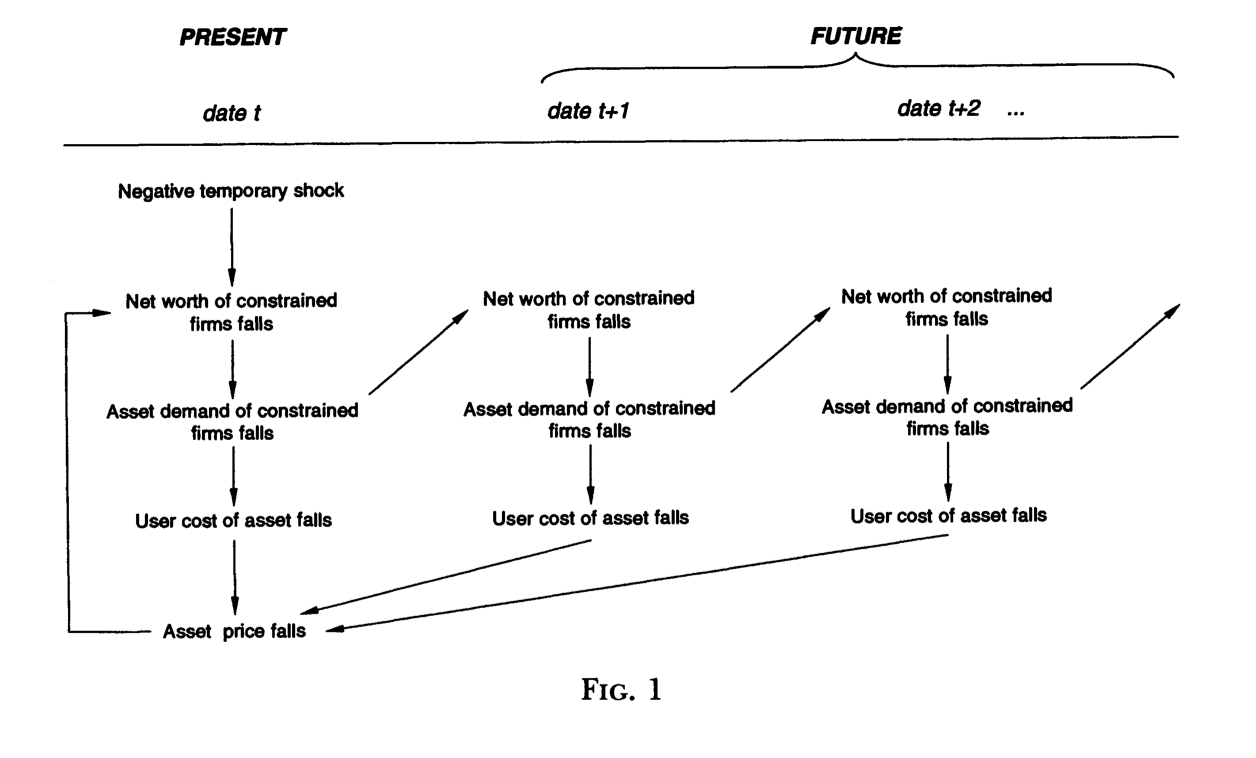
\includegraphics[width=\textwidth]{kiyotaki-moore-97.png}

\noindent
\textbf{Skills:}
\begin{itemize}
	\item How they deal with specific-targeted loan (i.e. the loan can only be used to purchase land)
\end{itemize}


% section collateral_constraints (end)


\section{Gorton and Ordonez, 14 AER} % (fold)
\label{sec:gorton_and_ordonez_14}

\textbf{\bibentry{10.1257/aer.104.2.343}}\\


\textbf{Motivation}: How a small shock can sometimes have a very huge, sudden effect, while at other times the effect of the same size shock is small or nonexistent. Leverage per se is not enough to explain this. This paper explains how credit booms arise, leading to financial fragility where a small shock can lead to huge consequences. Thus, "tail risk" is endogenous. The same reason causes boom and huge recession, and the degree of recession is positively correlated with the boom lasting time.

\textbf{Mechanism}: 

\begin{enumerate}
	\item Firm needs land as collateral to borrow money from households. Land is either good or bad. Neither firm nor household know the quality of land, and checking fee is $\gamma>0$. It can be shown that, when the probability of a land to be good is too high or too low, it will be optimal (for both firm and household) to not check the quality.
	\item Then suppose there are idiosyncratic shocks to land. For each land in each period, there is $\lambda$ prob to be unchanged, and $1-\lambda$ to be changed. In case of changing, $\hat p$ prob becoming good and $1-\hat p$ becoming bad, independent of initial type. So we can take it as a $\hat p$ type, it will become either 0 or 1 after checking. If $\hat p$ lies in some range that no checking is appropriate, then uncertainty in the economy will accumulate. Notice such accumulation will lead to a boom.
	\item Now think of an aggregate shock. All good type and $\hat p$ type have weaker beliefs after such shock, changing to $\eta$ and $\eta \hat p$ respectively. Notice that $\eta$ and $\eta \hat p$ may have very different effect. It may be optimal to not check with $\eta$ but optimal to check with $\eta \hat p$. Thus if an economy has accumulated a large portion of $\hat p$, i.e. a long boom, then many of them will choose to check, inducing a huge crisis.
	\item Notice that it is not because of any \textit{intrisinc} change in economy. The $\hat p$ will change the real portion of good land in the economy only once. What really matters is that once the bad one becomes $\hat p$, then even it switches back to bad in following periods, it will still be taken as $\hat p$. That means, the $\hat p$ type will accumulate in the economy.
\end{enumerate}

\textcolor{red}{Why this paper is important}:
\begin{itemize}
	\item Provide a way to endogenize information in general equilibrium model.
\end{itemize}


% section gorton_and_ordonez (end)

\section{Williamson, 87 QJE} % (fold)
\label{sec:williamson_87_qje}

\textbf{\bibentry{10.2307/1884684}}\\

\cite{10.2307/1884684} mainly wants to explain two things:
\begin{itemize}
	\item Why is debt contract so popular?
	\begin{itemize}
		\item By MM Theorem, we know that in a frictionless world, debt contract is equivalent to equity contract. But we notice that most fund is raised through debt.
		\item Explain by moral hazard. Borrower has private information on outcome. And lender has to pay for checking.
	\end{itemize}
	\item Why there is credit rationing?
	\begin{itemize}
		\item If the borrowing demand exceeds lending supply, why doesn't the interest rate increase to clear the market?
		\item Because checking is costly, so incentive compatibleness requires interest rate not being too high.
		They prove that the optimal interest rate is hump shape.
	\end{itemize}
\end{itemize}

An IC contract $\{S,K(w),R(w)\}$ contains three parts. $S$ is the checking area. $K(w)$ is the transfer to lender when not checking. $R(w)$ is the transfer to lender when checking. Since the contract is IC, so the reported $\hat w$ is just actual realized $w$.

There are three steps to prove the optimal contract is debt contract in this asymmetric information case.
\begin{enumerate}
	\item Prove $K(w)$ equals a constant x. [easy]
	\item Prove the IR constraint of lender will be tight. [easy]
	\item Prove $R(w)=w$, i.e. lender will take away everything in checking case. [difficult] 
\end{enumerate}

In the third step, the idea is easy. Because if lender takes away everything in checking case, then the checking area can be smaller, thus can save checking cost. The difficulty is: when we lower x (to make checking area A smaller), the non-checking area B becomes larger. The changes are in two different directions and problem becomes subtle. \textcolor{red}{In discussion we use the total differentiation approach to solve this. Important}.\\

\noindent
\textbf{Techniques:}

\textbf{how to prove optimal contract format:}

See above.\\

\textbf{recursive structure in defining EQM:}

One difficulty in determining the optimal contract is how to characterize outside options of lender. In equilibrium, When a lender decides whether to accept a contract from a specific borrower (entrepreneur), his outside option should be market interest rate $r$. Because entrepreneur can't identify lender, and all entrepreneur are homogeneous ex ante, so if the expected return from a specific contract should be larger than mkt interest rate $r$. Thus the IR of lender is:

\[\int_A R(w)d(F(w))+\int_B xd(F(w))-\gamma Pr(A) \geq r\]

$r$ has to be pinned down in the eqm. Because all agents have rational expectation, thus the market clearing $r$ will be the same as their expectation.

The equilibrium is defined as:
\begin{itemize}
	\item 
\end{itemize}


% section williamson_87_qje (end)


\section{Chari et.al, 14 AER} % (fold)
\label{sec:chari_et_al_14_aer}

\textbf{\bibentry{Chari_etal2014:aer}}

\vspace{3mm}
\noindent
\textbf{Empirical Facts:}
\begin{itemize}
 	\item simultaneous fluctuation between secondary loan market and underlying land market
 	\item persistence of collapse in secondary loan market trade volume
 \end{itemize}

 \noindent
 \textbf{Main Mechanism:}
 \begin{itemize}
 	\item adverse selection AND reputation
 	\item key assumptions:
 	\begin{itemize}
 		\item agent (bank) types persist over time
 		\item players are non-annonymous (possible to build reputation)
 	\end{itemize}
 	\item adverse selection: can account for trade volume fluctuations correlated with underlying collateral value
 	\item reputation:
 	\begin{itemize}
 		\item wihout reputation concern, adverse selection will be solved quickly. Because the first stage features a separating equilibrium
 		\item with high enough reputation concern (patient enough), first stage cannot be fully separate, so adverse selection problem persists
 	\end{itemize}
 \end{itemize}



% section chari_et_al_14_aer (end)





\chapter{Euro Crisis} % (fold)
\label{cha:euro_crisis}

This section is based on a course material of Wang Jue. Basically it discusses the theoretical concerns of Optimal Currency Area (OCA), why Europe adopts it, its success and its failure, and the recent Euro crisis.\\

\textbf{\bibentry{Krugman:2012eu}}

\cite{Krugman:2012eu} discusses the crisis of Euro area. Based on OCA theory by Mundell, there are two big things to look at: \textbf{labour mobility} and \textbf{fiscal integration}. Because areas are likely to suffer local idiosyncratic shocks. 
\begin{itemize}
	\item Without labor mobility, a state has to make wage fall to restore the full employment, this will be much easier with its own to devalue. But if labor mobility is high, then workers can just move to other states.
	\item Fiscal integration will also help. First because federal transfer is like a insurance, also because the borrowing cost for federal government is much lower.
\end{itemize}
The Euro crisis faces challenges in both parts.
\begin{itemize}
	\item The labor mobility is not high enough.
	\item No fiscal integration. And the asymmetric shock is so severe, making fiscal burden so large that calls government solvency into question. (e.g. in Spain and Greek)
	\item The bank issue. There is no `last resort', so the fear of sovereign default undermineds confidence in private banks which hold these bonds. This is called \textit{doom loops}.
	\begin{itemize}
		\item Compare between euro area countries and pegged-to-euro countries. Austria and Finland uses euro, but Finland just pegged to euro. This flexibility makes interest rate much lower during the crisis.
	\end{itemize}
\end{itemize}

\vspace{2mm}
\textbf{\bibentry{baldwin2015eurozone}}


\chapter{Macro Seminar Notes} % (fold)
\label{cha:macro_seminar_notes}

\noindent
\textbf{Cryptocurrency}

\begin{itemize}
	\item By Jesús Fernández-Villaverde and Daniel	Sanches 2017
		.Use Lagos and Wright (2005) framework.
	\begin{itemize}
		\item \url{http://economics.sas.upenn.edu/~jesusfv/Cryptocurrencies.pdf}
		\item Not positive on private currencies. First, competitive private money will not provide price stability, either with a profit-maximizing entrepreneurs or through automaton.
		\item Even with price stability, value of private money may go zero in infinite equilibriums.
		\item Purely private money system does not provide social optimal quantity of money.
	\end{itemize}
\end{itemize}

\myline

\textbf{\bibentry{Sorkin:18qje}}

\begin{itemize}
	\item Use Google Page Ranking algorithm to rank good firms. `good firms hire from other good firms and have few workers leave'. Reduce computation burden greatly.
	\item Previous literature use hedonic approach to rank firms. Two drawbacks:
	\begin{itemize}
		\item Need to completely model and measure all relevant elements
		\item Do not consider the utility dispersion case. [not understand]
	\end{itemize}
\end{itemize}

\textcolor{blue}{Worth reading.}



% section seminar_notes (end)



% section euro_crisis (end)


\part{Methodology} % (fold)
\label{part:methodology}


\chapter{Micro Foundations of Macroeconomics} % (fold)
\label{cha:micro_foundations_of_macroeconomics}

% section micro_foundations_of_macroeconomics (end)

\noindent
\textbf{Reductionism, and Micro Fundations of Economics:}

Economists are fascinated in forming `micro fundations' for almost all models. But do we really need this, does this effort pay? 

As pointed in famous paper \cite{anderson1972:science}: `\textit{The ability to reduce everything to simple fundamental laws doesn't imply the ability to start from those laws and reconstruct the universe... At each level of complexity entirely new properties appear... There is no useful parallel to be drawn between the way in which complexity appears in simplest cases of many modies and chemistry and culture ones.}'
The aggregated economy is so complicated that may not be reduced to individual decision problems.
\footnote{Zhao Dingxing has an article discussing this problem.

See \url{https://www.evernote.com/l/ATUOIdQb8hBM5r3QQv8cTK52Amq4-qlwb0E}}

Another problem worth thinking is the relationship between Sonnethein-Debreu theorem and macro economics models.


\vspace{2em}
\noindent
\textbf{Policy Making without Macroeconomic Theory:}
\footnote{\href{https://docs.google.com/viewer?a=v&pid=sites&srcid=ZGVmYXVsdGRvbWFpbnxrb2NoZXJsYWtvdGEwMDl8Z3g6NDhhODQ0MTI1MWMyNDRjNQ}{Click for link to slides}}


Kocherlakota (2018) points out that policy makers does not need to know economic theory, albeit the players are in the framework of theory.
The key points of the theory are:
\begin{itemize}
	\item Private sectors are forward looking, but government is myopic
	\item Gov suffers private taste shock, which will only affect the gov utility
	\item Within an equilibrium, government can pick the optimal policy through simple regression over past actions and stages
\end{itemize}



\chapter{Decision Theory as a Foundation} % (fold)
\label{cha:decision_theory_as_a_foundation}

% section decision_theory_as_a_foundation (end)


\vspace{3mm}
\noindent
\textbf{Meaning of Decision Theory:}

(This part is heavily influenced by Henrique's class.)

Why we need to do decision theory?
Take an \textit{inverse engineering} perspective.
Suppose we have a model, which uses utility function to describe people's decison choices. 
That is, $u:X \rightarrow \R$.
And we define $C(B)=\argmin_{x\in B} u(x)=
\{x\in B | u(x)\geq u(y),\forall y\in B\}$.
We can map such functions to a \textit{equivalent class}, and can further map it to a \textit{preference relation} (a subset of relations).

The problem is such mapping is not surjective.
Every utility function has a corresponding equivalence and a prefence relation,
but there is some preference relation that cannot be represented by a utility function.
Thus we need to put some restrictions over preference relation.

The first relation is that the cardinality of indifference curves cannot be larger than $\R$.
This is easy to understand.

But this restriction is not enough.
Think of lexicographic preference,
every point in the two-dimension space is a indifference class.
The cardinality of which is $R^2$, equivalent to cardinality of $\R$.
But we know that such preference do not have a corresponding utility function.
We can further restrict preference to \textit{order separable} relations,
then by Debreu Thm, we can show the \textit{iff} between utility and preference relations.

\begin{defn}[Order Separable]
A preference relation defined over $X$ is order separable if $\exists Y \subseteq X$ countable s.t. $\forall x_1,x_3 \subseteq X$,
we have $x_1 \succ x_2 \Rightarrow \exists y \in Y$
 s.t. $x_1 \succ y \succ x_2$.
\end{defn}

Important here is thaat by assuming the range of utility function is $\R$ (such a weak condition),
we actually put some restrictions over preference.

\vspace{3mm}
\hrule
\vspace{3mm}

\vspace{2mm}
\noindent
\textbf{Calibration:}

\noindent
Why use calibration instead of estimation?
\begin{itemize}
	\item Because we live in a `tenth-best' world, and our model only catches a small part of the world.
	Use calibration we can fit the moments that our model fail to catch,
	in this sense to be more accurate.
\end{itemize}

May use calibration parameters as an intuitive check of whether the code we wrote is correct.


\myline

\noindent
\textbf{Research Reproducibility}

\cite{Maniadis:2017gq} claims two aspects of reproducibility problem.
First, it can be seen as an `evidence game', 
where researchers have some private information
and evaluators have to design a incentive compatible mechanism for publishing and granting.
Second, empirical methods from meta-research may help. 
(I don't understand the second part.)

\cite{Maniadis:2017hi} in the same issue provides more detailed guide on what will affect the credibility of scientific research.
It raises a concept post-study probability,
\[PSP=\frac{(1-\beta)\pi}{(1-\beta)\pi+ \alpha(1-\pi)}\]
where $\alpha$ is significance level, $1-\beta$ is power,
and $\pi$ is the probability that a research question is actually true. $\pi$ can be think of as \textit{prior} given by theory.
This is the fraction of `truly true and reported true' divided by `all reported true'.
Easy to see, when $\pi$ is low, 
the PSP can be very low even with low $\alpha$.
This indicates that with those fields where theory can provide little guide,
we have to be very skeptical to the `rejection' outcomes.
They are very likely to be `false positive'. 

\cite{Spiess:2017tp} has a fantastic discussion of this from the perspective of econometrics and mechanism design.


\myline

\noindent
\textbf{Lucas Critique:}

\cite{Hoover:94JEMethod} views Lucas critique as pointing the causal inference and identification problem in econometrics.

% chapter methodology (end)









% chapter macro (end)
\part{Mathematics}

\chapter{General (mathematical) Skills} % (fold)
\label{cha:general_mathematical_skills}

\section{Log-Linearization}

\noindent
\textbf{Motivation}

Why we need log linearizations?
Because for most nonlinear discrete dynamic programming problems,
we fail to find a closed solution.
Thus we have to use numerical method or to find a approximation.
By using log-linearization,
we transform the nonlinear problem to a linear problem (around the steady state),
and we know how to solve the linear diffrence equations.

Another advantege of log-linearization is,
the new variables are in forms of $\frac{x-x^*}{x^*}$,
which is interpretable.\\


% subsection: how to do log-linearization
\subsection{How to do Log-Linearization}

Log linearization is a common method to approximate non-linear function using Taylor expansion.

When we do linearization in macroeconomics, one key is to find \emph{\textbf{steady state}} of the model.
Then we do linearization aroud the steady state.

The basic idea is, for functions like:
\[f(x)=\frac{g(x)}{h(x)}\]

take log in both sides:
\[ln(f(x))=ln(g(x))-ln(h(x))\]

By Taylor expansion, for a smooth function f(x) we have:
\[f(x)=f(x^*)+\frac{f'(x^*)}{1!}(x-x^*)+o(1)\]

Thus 
\[lnf(x) \approx lnf(x^*)+\frac{f'(x^*)}{f(x^*)}(x-x^*)\]

The above follows from the fact that $\frac{dln(f(x))}{dx}=\frac{f'(x)}{f(x)}$. Thus,
\[lnf(x)-lnf(x^*)=\frac{f'(x^*)}{f(x^*)} \cdot x^* \cdot \frac{x-x^*}{x^*}\]

And the equation becomes:
\[lnf(x^*)+\frac{f'(x^*)}{f(x^*)} \cdot x^* \cdot \frac{x-x^*}{x^*}=lng(x^*)-lnh(x^*)
\frac{g'(x^*)}{g(x^*)} \cdot x^* \cdot \frac{x-x^*}{x^*}-
\frac{h'(x^*)}{h(x^*)} \cdot x^* \cdot \frac{x-x^*}{x^*}\]

\[\frac{f'(x^*)}{f(x^*)} \cdot x^* \cdot \frac{x-x^*}{x^*}=
\frac{g'(x^*)}{g(x^*)} \cdot x^* \cdot \frac{x-x^*}{x^*}-
\frac{h'(x^*)}{h(x^*)} \cdot x^* \cdot \frac{x-x^*}{x^*}\]

Dedine $\hat x=\frac{x-x^*}{x^*}$, and we are done.
\[\frac{f'(x^*)}{f(x^*)} x^* \cdot \hat x=
\frac{g'(x^*)}{g(x^*)} x^* \cdot \hat x-
\frac{h'(x^*)}{h(x^*)} x^* \cdot \hat x\]

Notice, when we use $\hat x$ in place of $x-x^*$in the approximation,
don't forget to times $x^*$ !!\\

% How to do log-linearization when there is Expectation

\subsection{log-linearization when there is expectation (An Example)}

It may be annoying to do log-linearization when there is expectation,
because in general,
log and expectation cannot switch.
But if we don't switch, we cannot do the log-linearization as previous.
For example, see Adda\&Cooper(2003) CH5, page 115.

Suppose we have the following Euler equation:

\[u'(c)=\beta E_{A'|A}u'(c)[Af'(k')+(1-\delta)]\]

where $c=Af(k)+(1-\delta)k-k'$.

These two expressions, along with the evolution of A,
defines a system of equations.

In this system, actually we do not have to take log,
but directly do Taylor expansion at $c^*$, $x^*$ and $k^*$.
We get:

\begin{multline}
u'(c^*)+u''(c^*)c^*\hat c_t=
\beta E_{A'|A}[u'(c^*)(\bar Af'(k^*)+(1-\delta))
+(\bar Af'(k^*)+(1-\delta))u''(c^*)c^*\hat c_{t+1}\\
+u'(c^*)f'(k^*)\bar A\hat A_{t+1}+
u'(c^*)\bar Af''(k^*)k^* \hat k_{t+1}]
\end{multline}


The first term in LHS and the first term in RHS cancel each other.
And we divide both sides by $u'(c^*)$, and we will get:

\begin{equation}\label{eq1}
\frac{u''(c^*)c^*}{u'(c^*)}\hat c_t
=\beta E_{A|A'}[\frac{u''(c^*)c^*}{u'(c^*)}\hat c_{t+1} \frac{1}{\beta}
+f'(k^*)\bar A \hat A{t+1}
+f''(k^*)k^*\hat k_{t+1}]
\end{equation}

Notice, we derive this based on the fact $\frac{1}{\beta}=\bar A f'(k^*)+(1-\delta)$.
Because by FOC
\[u'(c)=\beta E_{A'|A}V'(k')\]

To derive $V'(k')$, we first derive $V'(k)$,
by Envelop THM we get:
\[V'(k)=u'(c)[Af'(k)+(1-\delta)]\]

Substitute this into FOC we get:
\[u'(c)=\beta E_{A|A'}[u'(c')(A'f'(k')+(1-\delta))]\]

In this approach we fix A at the mean $\bar A$,
and thus the steady state satisfy:
\[1=\beta [\bar Af'(k^*)+(1-\delta)]\]

Here, the introduce of $\bar A$ is to describe the steady state in existence of shock.
We can see $\bar A$ as the "long term" growth of the economy,
and the we investigate what's the optimal steady $k^*$ under this long-term growth rate.

\textcolor{red}
{But I still don't know why we can cancel the expectation in the RHS.}

The equation \ref{eq1} is the linear function we want.\\

\noindent
\emph{Some Comments on the above method:}

Although it seems that the above method uses no log-linearization,
actually it does!

(to be added later)

% section log-linearization (end)



\section{Supermodularity} % (fold)
\label{sec:supermodularity}

\noindent
Reference: 
\begin{itemize}
	\item \href{run:resources/sobel_supermodularity.pdf}{Sobel's Notes:} \url{http://econweb.ucsd.edu/~jsobel/205f10/notes12.pdf}
	\item \href{run:resources/monotone_comparative_statics.pdf}{A more detailed note:} \url{https://pages.wustl.edu/files/pages/imce/nachbar/monotonecomparativestatics.pdf}
	\item \bibentry{topkis1998:supermodularity}
\end{itemize}


\section{Miscellanea} % (fold)
\label{sec:miscellanea}

\subsection{Elasticity} % (fold)
\label{sub:elasticity}

\begin{exmp}
Suppose $Q=\sum{q_i}$, $p=Q^{1/\alpha}$ and define $s_i=\frac{q_i}{Q}$. In equilibrium, we have $s_i=s_i^*$.
Then in equilibrium, we have $\frac{\partial p}{\partial q_i}=s_i^*/\alpha$ instead of $1/\alpha$.

Why? In first look, $Q$ is linear in $q_i$, then the derivative $\partial p/\partial Q$ should be the same as $\partial p/\partial q_i$.
The point is that $Q$ is just a aggregated notation.
In equilibrium, small change in $q_i$ will induce small change in all $q_{j \neq i}$, thus the aggregate change in $Q$ will be proportion of change in $q_i$.
\end{exmp}

% subsection elasticity (end)

% section miscellanea (end)


% section supermodularity (end)



% chapter general_mathematical_skills (end)


\chapter{Probability} % (fold)
\label{cha:probability}

\begin{thm}[Linear Combination of Dependent Normal RV]
Suppose \(\left(\begin{matrix}X\\Y \end{matrix}\right) \sim \mathcal{N}\left[ \left(\begin{matrix}\mu_X\\\mu_Y\end{matrix}\right), \Sigma_{X,Y} \right]\),
then
\(AX+BY+C \sim \mathcal{N}\left[ 
\left(\begin{matrix}A& B \end{matrix}\right)
\left(\begin{matrix}\mu_X\\\mu_Y\end{matrix}\right) + C, 
\left(\begin{matrix}A & B \end{matrix}\right)\Sigma_{X,Y} \left(\begin{matrix}A^T \\ B^T \end{matrix}\right)\right]\).
\end{thm}


\begin{thm}[Kolmogorov's zero–one law]
Let $(\Omega,F,P)$ be a probability space, and $F_n$ be a series of independent $\sigma$-algebras contained in $F$.
Let
\[G_n = \sigma \left( \cup^\infty_{k=n} F_k\right)\]
Then we define tail event $F$ to be any event such that:
\[F \in \cap^\infty_{n=1}G_n\]
Kolmogorov zero-one law claims that $Pr(F)=0$ or $Pr(F)=1$. 
\end{thm}

Intuitively, if the occurrence of a event $F$ can be determined when any finite initial segment is removed, then it either happens or not with probability 1.


\section{Distributions} % (fold)
\label{sec:distributions}

\begin{itemize}
	\item Pareto Distribution
	\item T1EV (Type 1 Extreme Value)
\end{itemize}


% section distributions (end)



\section{Bayesian Statistics} % (fold)
\label{sec:bayesian_statistics}

\subsection{Bayesian Updating} % (fold)
\label{sub:bayesian_updating}

\begin{thm}[Bayesian Update in Odds]
For hypothesis $H$, data $d$ and prior odds $O(H)$. We have posterior odds 
$O(H|d) = O(H)\cdot\frac{Pr(d|H)}{Pr(d|H^c)}$,
where the second term is called \textit{Bayes Factor}.
\end{thm}

\begin{myproof}
\begin{align*}
	O(H|d)&=\frac{Pr(H|d)}{Pr(H^c|d)} \\
	&=\frac{Pr(d|H)Pr(H)}{Pr(d|H^c)Pr(H^c)}\\
	&=\frac{Pr(d|H)}{Pr(d|H^c)}\cdot O(H)
\end{align*}
\end{myproof}



% subsection bayesian_updating (end)


% section bayesian_statistics (end)


% chapter probability (end)


\chapter{Numerical Methods} % (fold)
\label{cha:numerical_methods}


\noindent
\textbf{Computation laguage:}
\begin{itemize}
	\item \url{http://economics.sas.upenn.edu/~jesusfv/comparison_languages.pdf}
	\begin{itemize}
		\item discusses efficiency of different languages
		\item hybrid language can significantly increase efficiency
	\end{itemize}
\end{itemize}

\noindent
\textbf{Matlab Speed Up:}
\begin{itemize}
	\item Microeconometrics and Matlab: an Introduction, Ch-10
	\item vectorize and preallocate values
		\begin{itemize}
		 	\item Cooper's growth model uses clever vectorizing, avoid one loop
		 \end{itemize} 
	\item profiling code: profile on, main, profile off
	\item parallel computing
\end{itemize}

\section{Numerical Maximization} % (fold)
\label{sec:numerical_maximization}

\noindent
\textbf{Newton-Raphson Method:}

Idea: use quadratic function to approaximating real function at current guess,
then find the maximization point of this quadratic function as next guess.
\[\beta_{t+1}=\beta_t + \lambda(-H^{-1}_t)g_t\]
where $H_t$ is the Hessian of the function to be evaluated at $\beta_t$, 
and $g_t$ is the Jacobian at $\beta_t$,
$\lambda$ is the step size, generally may take 1.

\vspace{3mm}
\noindent
\textbf{BHHH Method:}

Idea: almost the same as Newton-Raphson, but use the outer product to approximate Hessian.
\[\beta_{t+1}=\beta_t + \lambda(-B^{-1}_t)g_t\]
where $B_t = \frac{1}{N}\sum_{n=1}^N{s_n(\beta_t)s_n(\beta_t)'}$
and $s_n(\beta_t)= \partial P_n(\beta)/\partial \beta$ evaluated at $\beta_t$,
and $g_t=\frac{1}{N}\sum_{n=1}^N{s_n(\beta_t)}$.

Key is, when evaluated at maximum value, $s_n$ should be zero. Thus $B_t$ evaluated at maximum is the variance of $s_n$ in the sample, which is just the Hessian of the sample likelihood function.
This is just \textit{information equality}.

\begin{itemize}
	\item [\textbf{pros:}] BHHH is generally faster than Newton-Raphson near the maximum.
	Because $s_n$ have to be calculated anyway, 
	but in NR procedure we have to calculate the second derivatives as well.
	\textcolor{blue}{But seems this is not the case, in experiments BHHH always slower than Newton-Raphson.}
	\item [\textbf{cons:}] BHHH is generally slower when $\beta_t$ is far from true value. 
	Because at these points $B_t$ is not a good approximate of $H_t$.
\end{itemize}

% section numerical_maximization (end)


\begin{itemize}
	\item Root Solving
	\item Integration
	\begin{itemize}
		\item Gaussian quadrature
		\item Sparse grid
		\item Monte Carlo integration
		\begin{itemize}
			\item antithetic accelerating
			\item importantce sampling
		\end{itemize}
		\item Quasi Monte Carlo
	\end{itemize}
\end{itemize}


% chapter numerical_methods (end)


\bookmarksetup{startatroot}% this is it
\addtocontents{toc}{\bigskip}% perhaps as well


\chapter{Miscellany} % (fold)
\label{cha:miscellany}

\noindent
\textbf{Presentation:}
\begin{itemize}
	\item Always \textit{motivate} very clearly, both from economics facts and from literature.
	\begin{itemize}
		\item In macro, a graph generally helps
	\end{itemize}
	\item Make clear propositions so that others won't misunderstand.
	\begin{itemize}
		\item Bad: analyze the competitive pattern of inter-brand and intra-brand

		Good: Analyze how the per store profit is affected by own-brand store density and competitors' store density
	\end{itemize}
	\item If possible, always use a simple model at the beginning
	\begin{itemize}
		\item To pin down the concepts/definitions
		\item To show the mechanism intuitively
	\end{itemize}
	\item Understand the result both mathematically and intuitively
	\item Visualization:
	\begin{itemize}
		\item If only the scale of number is important, use a \textit{plot} instead of table full of numbers
	\end{itemize}
	\item When writing on the board, write horizontally!
\end{itemize}


\vspace{1em}
\noindent
\textbf{Writings:}
\begin{itemize}
	\item Good writing samples: \cite{Berry:1992gl}, \cite{doi:10.3982/ECTA7699}
	\begin{itemize}
		\item \cite{doi:10.3982/ECTA7699}: a good example of illustrating clear empirical results
	\end{itemize}
\end{itemize}


% part miscellany_ (end)


\renewcommand\refname{Reference}
\bibliographystyle{chicago}
\bibliography{reference}


\end{document}
